                                                   
                                             
\documentclass[12pt,notitlepage,a4paper]{report}
\pagestyle{plain}

\frenchspacing % aktivuje použití některých českých typografických pravidel

\usepackage[utf8]{inputenc} % nastavuje použité kódování, uživatelé Windows zamění latin2 za cp1250
\usepackage[english,czech]{babel}

%\usepackage{index} % nutno použít v případě tvorby rejstříku balíčkem makeindex
%\usepackage{fancybox} % umožňuje pokročilé rámečkování :-)
\usepackage{graphicx} % nezbytné pro standardní vkládání obrázků do dokumentu
\usepackage{ifpdf} % přidá možnost diference podle finálního formátu
\ifpdf
\usepackage{epstopdf}
\fi
\usepackage{lib/DocumentPropertiesInserting} % umožňuje vkládat hodnoty title a author atd. do dokumentu.

\usepackage{datetime} % Umožňuje formátovat data

\usepackage{indentfirst} % zajišťuje odsazení prvního odstavce za nadpisem.

\usepackage[left=4cm]{geometry} % nastavení dané velikosti okrajů

\usepackage{url} % Usnadňuje vkládání URL.

\usepackage{rotating} % Podpora vertikálního textu.

\usepackage{pifont} % Umožňuje použít symboly

\usepackage{color} % Dovoluje používat barvy.

\usepackage{amsmath,amsthm}% Umožňuje číslování příkladů.

\usepackage[font=small,format=plain,labelfont=bf,up,textfont=up]{caption}

\usepackage{fancyvrb}

\usepackage{alltt}

\usepackage{amssymb}

\usepackage{enumitem}

\usepackage[toc,page]{appendix}

\renewcommand{\ttdefault}{txtt}
\sloppy

%\newindex{default}{idx}{ind}{Rejstřík} % zavádí rejstřík v případě použití balíku index

\title{Modelem řízený formátovač kódu pro Xtext framework}
\englishtitle{Model-driven Pretty Printer for Xtext Framework}
\author{Marek Novotný}
\institute{Charles University in Prague}
\faculty{Faculty of Mathematics and Physics}
\department{Katedra distribuovaných a spolehlivých systémů}
\englishdepartment{Department of Distributed and Dependable Systems}
\supervisor{RNDr. Michal Malohlava, Ph.D.}
\supervisorsemail{michal.malohlava@d3s.mff.cuni.cz}
\newdate{creationdate}{04}{12}{2012} % TODO: Opravit datum napsání dokumentu
\date{\displaydate{creationdate}}




\begin{document}
\selectlanguage{english}
% Titulní stránka.
\begin{titlepage}
\begin{center}
\ \\
\vspace{\fill}

\large
\insertinstitute\\
\insertfaculty\\

\vspace{5mm}

{\Large\bf MASTER THESIS}

\vspace{10mm}


\includegraphics[scale=0.3]{pictures/Logo_MFF.eps}

\vspace{15mm}

{\Large \insertauthor}\\
\vspace{5mm}
{\Large\bf \insertenglishtitle}\\
\vspace{5mm}
\insertenglishdepartment\\
\end{center}
\vspace{15mm}

\large
\noindent Supervisor: \insertsupervisor
\vspace{1mm} 

\noindent Study program: Computer Science\\
Specialization: Software Systems

\vspace{\fill}

\begin{center}
\getdateyear{creationdate}
\end{center}

\end{titlepage}




% Formality.
\normalsize
\setcounter{page}{2} % nastavení číslování stránek
\ \vspace{10mm} 

\noindent I would like to thank the thesis supervisor RNDr. Michal Malohlava, Ph.D. for his valuable comments and suggestions. His experience with Xtext framework and overall with model-driven development have proved to be of high importance for me. Finally, I want to thank my family for their support.

\vspace{\fill}

\noindent Prohlašuji, že jsem svou diplomovou práci napsal samostatně a výhradně s použitím citovaných pramenů. Souhlasím se zapůjčováním práce a jejím zveřejňováním.

\ \vspace{0mm}

\noindent I declare that I have elaborated this master thesis on my own and listed all used references. I agree with lending and publishing of this thesis.

\bigskip
\noindent In Prague on 4th December 2012 \hspace{\fill}\insertauthor\\ % TODO: Změnit datum

\tableofcontents

\newpage

\noindent
Název práce: \inserttitle\\
Autor: \insertauthor\\
Katedra (ústav): \insertdepartment\\
Vedoucí diplomové práce: \insertsupervisor\\
E-mail vedoucího: \insertsupervisorsemail\\

\noindent Abstrakt: Doménově specifický jazyk slouží k popisu problémů v doméně, pro níž byl vytvořen. Tento fakt implikuje, existenci velkého množství jazyků tohoto druhu. Používání doménově specifických jazyků přináší s sebou potřebu tyto jazyky formátovat a zvýrazňovat jejich syntaxi. Jedním z nástrojů, které umožňují tvorbu doménově specifických jazyků, je prostředí \textsc{Xtext}, který nabízí pouze omezenou paletu nástrojů umožňující nadefinovat formátování kódu a jeho zvýraznění. Navíc  jsou tyto nástroje pro uživatele těžko pochopitelné, jelikož jsou nepřehledné a vyžadují znalosti vnitřních záležitostí prostředí \textsc{Xtext}. Proto tato práce představuje nový způsob formátovaní a zvýrazňování kódu pro prostředí  \textsc{Xtext}, který je založen na deklarativní definici formátovacích pravidel. Kromě toho tato práce pomáhá uživateli s tvorbou formátovacích pravidel na základě netriviálních heuristik.


\vspace{5mm}

\noindent Klíčová slova:  eclipse, xtext, formátovač kódu, modelem řízený vývoj, doménově specifický jazyk

\vspace{10mm}

\noindent
Title: \insertenglishtitle\\
Author: \insertauthor\\
Department: \insertenglishdepartment\\
Supervisor: \insertsupervisor\\
Supervisor's e-mail address: \insertsupervisorsemail\\

\noindent Abstract: The domain-specific language allows  for  describing problems of a concrete domain, for which the language is created. This fact implies that a number of languages of this kind grows with a number of problem domains. The use of domain-specific languages brings a necessity to pretty-print these languages, where the concept of pretty-printing consists of code formatting and syntax highlighting.  One of tools that allow for creating domain-specific languages is the \textsc{Xtext} framework, which offers only a limited range of tools that are able to define a configuration for pretty-printing. Moreover, these tools are hardly understandable because they are confusing and requires knowledge of \textsc{Xtext}'s internals. Thus this thesis introduces  a new way of pretty-printing domain-specific languages. The way is based on declarative definition of formatting rules. Furthermore, this thesis helps a user to create formatting rules by utilizing nontrivial heuristics.

\vspace{5mm}

\noindent Keywords: eclipse, xtext, pretty printer,  model-driven development,  domain-specific language

\newpage



\newenvironment{memberlist}{
\begin{description}
	\setlength{\parsep}{0mm}
	\setlength{\parskip}{0mm}
	\setlength{\itemsep}{1mm}
}
{\end{description}}

\newenvironment{cdcontentlist}{
\begin{description}[font=\normalfont\texttt]
	\setlength{\parsep}{0mm}
	\setlength{\parskip}{0mm}
	\setlength{\itemsep}{1mm}
}
{\end{description}}

\newcommand{\member}[2]{\item [#1] \hfill \\ #2}

% Vlastní práce

\chapter{Introduction}

\section{Motivation}

Writing code is a craft which requires mature tools, conventions, and systematic approaches. One of crucial part of writing code is its representation which needs to be readable. The requirement can be solved by automatic \textit{code formatting}, which represents the way to enforce coding conventions. A configuration of a \textit{code formatter} represents coding conventions for a particular language used in a software project. The next mechanism improving the readability of code is \textit{syntax highlighting} which allows for distinguishing different code parts  by color, font, style, etc. Code formatting and syntax highlighting are basic elements of the concept called \textit{pretty-printing}. 

In these days most of development environments or language editors include a \textit{pretty printer} designed for a particular language.  These ad-hoc pretty printers tend to be hardly configurable and are mostly dedicated for only one language. Thus another crucial problem is to define a pretty printer for a general domain-specific language. Domain-specific language is a programming or specification language dedicated to a particular problem domain such as SQL, HTML, AWK, SED etc. Furthermore, this kind of languages can be created by utilizing the \textsc{Xtext} framework. A DSL often serves to describe a real life scenario with domain specific terms.  But it means that each DSL closely related to its problem requires creation of ad-hoc pretty printer from scratch which takes a lot of time.

Code of DSLs can be often reflected into a model which facilitates code manipulation and creation of tools serving for work with DSLs. This approach of software development is called \textit{model-driven development}. The core structure of final code can be generated from a model which reflects the process of design. This fact allows for reducing time-consuming and error-prone handwritten code. Although, the concept simplifies software development, the models of ad-hoc pretty printers contain many similarities. Therefore it would be beneficial to have a model-driven pretty printer that would be language independent and an implementation of differences derived from language features should be represented by an extension of the pretty-printer.
\section{Goals}

The aim of this thesis is to design a concept of a model-driven pretty-printer for the \textsc{Xtext} framework \cite{Xtext} dealing with creation of domain-specific languages. The concept should be confirmed by an appropriately incorporated implementation into the environment of the \textsc{Xtext} framework. Code of imperative languages contains much syntax ballast, thus pretty-printer settings for particular language features and formatting settings should be configured with the best declaratively.

\section{Structure of the Thesis}

The thesis is separated into eleven chapters. The current \textit{Chapter 1} introduces the topic of this thesis. The following two chapters describe state of art of formatting concepts located in the \textsc{Xtext} framework and other concepts important for a design of the model-driven pretty printer. Especially, the \textit{Chapter 2} deals with the formatting concepts of the \textsc{Xtext} framework and the \textit{Chapter 3} deals with the other concepts. The \textit{Chapter 4} revisits goals of the thesis and analyzes them in more detail. The analysis contained in this chapter implies creating three new domain-specific languages. A design and realization steps of the first language that allows for specifying a formatting tool of the pretty printer are contained in the \textit{Chapter 5}.  The design and realization steps of the second language that allows for specifying a formatting configuration for a particular language are contained in the \textit{Chapter 6}. The design and realization steps of the third language that allows for specifying some heuristic rules dedicated for generating an initial formatting configuration are contained in the \textit{Chapter 7}. A possible way how to integrate these languages into the \textsc{Xtext} framework and interconnect them with existing formatting concepts of the \textsc{Xtext} framework is described in the \textit{Chapter 8}. Evaluation of the prototype implementing proposed solution can be founded  in the \textit{Chapter 9}. The \textit{Chapter 10} discusses related work and the last \textit{Chapter 11} concludes the thesis and contains ideas for future work.

\chapter {Overview of Xtext Framework}
This chapter describes the \textsc{Xtext} framework \cite{Xtext}, which is a plug-in for \textsc{Eclipse IDE} \cite{Eclipse}, from user's point of view. Xtext is being developed by Itemis AG company and is freely available under the \textsc{Eclipse Public License} (EPL) \cite{EPL}.

\section {Domain of Use}
\label{DomainOfUse}
The \textsc{Xtext} framework is primarily intended for the development of small textual domain-specific or full-blown general purpose programming languages. A great advantage of the  \textsc{Xtext} framework is its continuity with \textsc{Eclipse Modeling Framework} (EMF) \cite{EMF} that enables conversion of code written in a particular language to a model, which can be further modified, transformed to another model or serialized to code of any language. The only matter which is necessary to establish a link between code and a model is to have a meta-model and refer to it in the rules of the given language grammar. The meta-model is essentially the description what the model structure should look like. If the structure of the final model is not important, a meta-model does not have to be defined by a user but can be generated from the grammar. The main ideas expressed in this paragraph are depicted in the \textit{Figure \ref{ModelAndCode}}.

\begin{figure}[h!]
\centering
\caption{A diagram expressing how a model, a meta-model, a grammar and DSL code are interconnected. The diagram utilizes a simple example with animals in a zoo.}
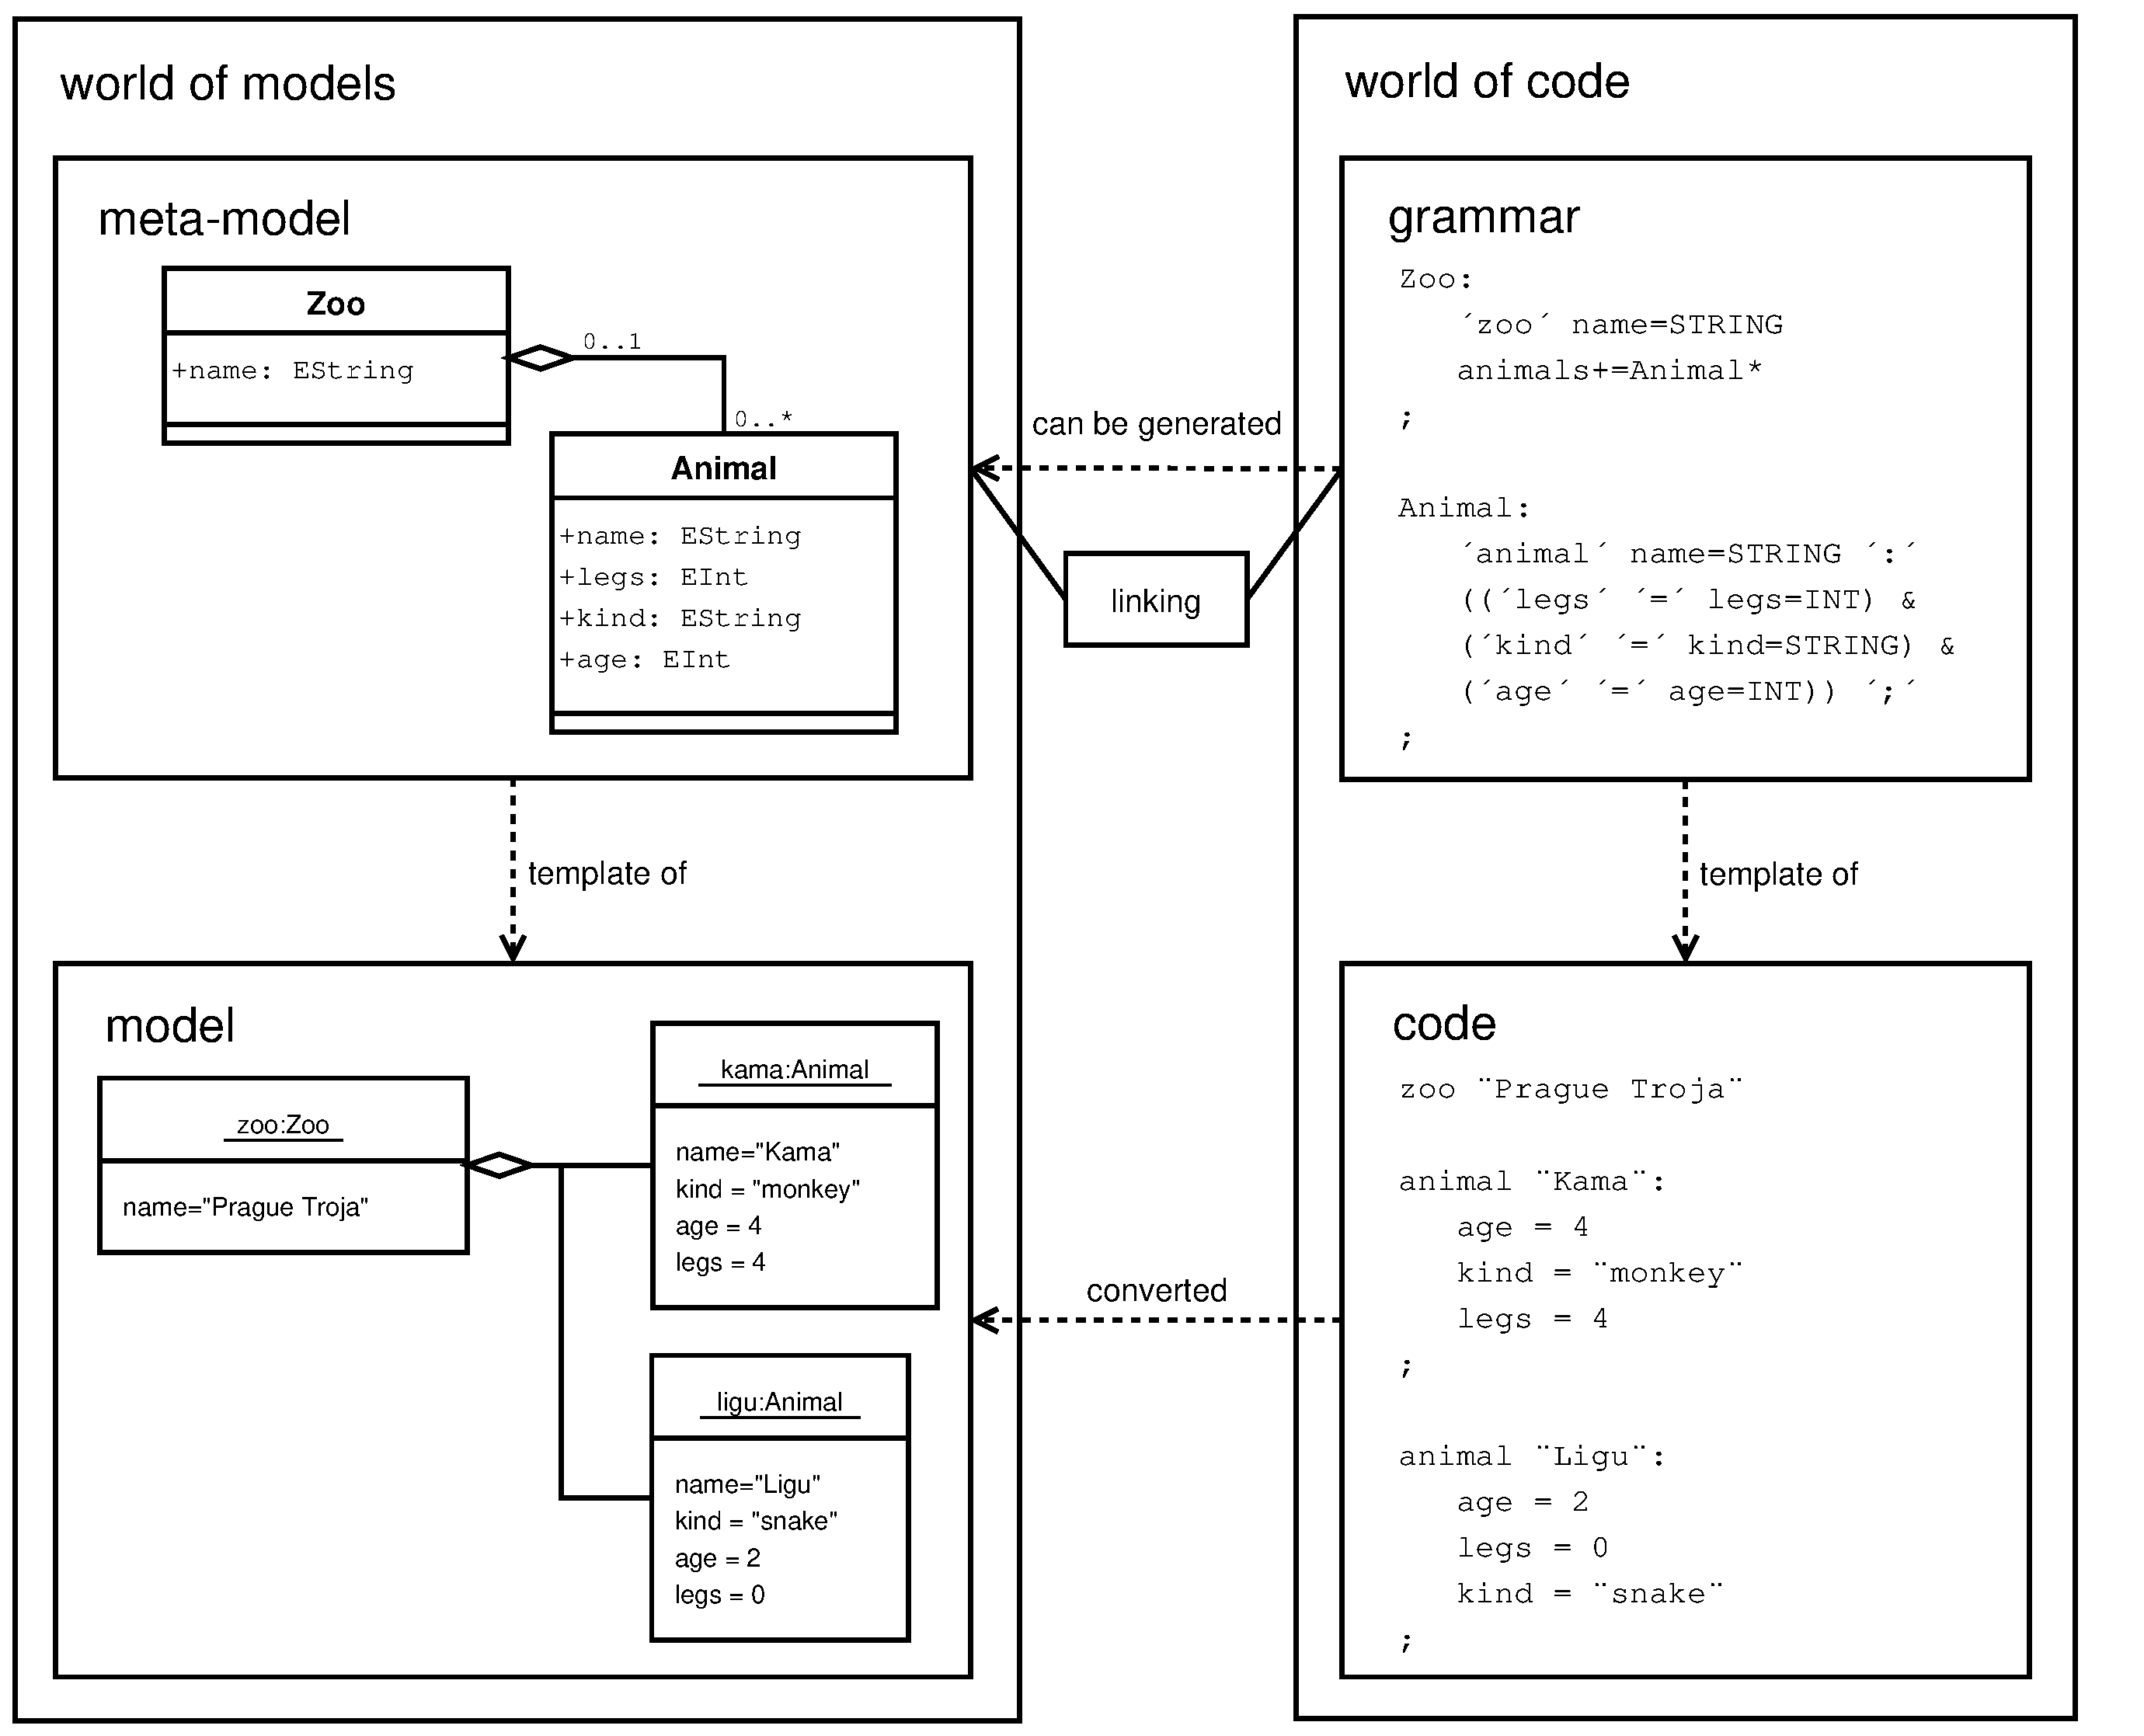
\includegraphics[scale=0.30]{pictures/ModelsAndCode.eps}
\label{ModelAndCode}
\end{figure}
\noindent

\section {Workflow}
\label{WorkflowConcepts}
Before a user starts to write a grammar it is good to have an idea of what the given language syntax should look like and what claims are imposed on it. A good approach is to first create code examples of the language, which will be later useful for grammar testing. After the user has written a correct grammar containing all necessary references to meta-models and other requisites, code of a  plug-in integrating the designed language into \textsc{Eclipse IDE} can be generated. The plug-in contains many runtime and IDE concepts, whose default behavior can be mostly changed by addition of standardly named methods into the prepared class. In this text, only the most important ones will be listed.

\subsection{Runtime Concepts}

These concepts deal with the \textsc{Eclipse} plug-in back-end and especially with the affairs of model generation from a code and code of a DSL as such. 

\subsubsection{Code Formatting}{As it was mentioned in the introduction, the code formatting concept deals with the organization of code elements in such way that the code is more legible.}
\subsubsection{Linking}{The concept serves to creating \textit{cross-references} related to already existing model elements. The cross-reference is essentially a link to another grammar rule specifying a nonterminal. When a language is given that allows for declaring variables and subsequently use them, declaration of a variable can serve as a target of a cross-reference and an usage of the variable is the cross-reference.}

\subsubsection{Scoping}{The concept defines visibility boundaries of reference targets for a particular cross-reference. The boundaries can be defined not only inside the file where the cross-reference is present but also over multiple files.}

\subsubsection{Validation}{The concept serves to check whether the model, which is a result of the input code, fulfill given features that  can not be defined through grammar rules such as the definition of a specific number of elements in the model, an order of elements in the model, etc.}

\subsection{IDE Concepts}

These concepts integrate a newly created language into the \textsc{Eclipse IDE} and provide convenience for a language developer working with a language. The main goal of the concepts is to speed up code writing.

\subsubsection{Content Assist}{The content assist serves to suggest and complete a code according to the possibilities specified by context which is determined by the cursor in the code.}

\subsubsection{Outline View}{The outline view is a tool that helps developers navigate through created models. It enables to view model elements hierarchically and sort them alphabetically.}

\subsubsection{Labeling}{This concept allows for associating a model element with the label or the icon that are exploited by other IDE concepts. For example these presentation elements can be found in the suggest window of content assist or in the window of outline view.}

\subsubsection{Quick Fixes}{This concept provides a possibility possibility of fixing code errors reported by explicitly defined validation rules as well as validation rules are derived from a grammar. The main principle of the concept is to produce the list of suggestions on the basis of an error type. Then it is up to the developer to choose one of the suggestions.}

\subsubsection{Template Proposals}{Consider well-known "while" statement from ordinary imperative languages. The only two things which can be written differently regardless of the code formatting is the loop condition and the loop body. Everything else is a matter of a particular language syntax which is always the same. This fact led authors of the \textsc{Xtext} framework to create the concept of templates. The developer of a created language can define templates for various statements or other language constructs. The user can use the template according to context and fill a new code into variable parts of the template. }

\subsubsection{Syntax Coloring}{This concept serves the same purpose as syntax highlighting mentioned in the \textit{Chapter 1}, in which different types of code are associated with  fonts, font colors, backgrounds, etc. }

\subsection{Configuration}
The \textsc{Xtext} framework offers a number of ways to change a standard behavior of the plug-in corresponding to a developed language.  One of them is a possibility to configure the \textit{Modeling Workflow Engine}.

\subsubsection{Modeling Workflow Engine}
\label{MWE}
The currently used Modeling Workflow Engine 2 (MWE2) is responsible for hierarchical startup of every action which is necessary for the generation of a language plug-in. The engine is basically the component model, whose design is based on the POJO~\cite{POJO}. By default, the runnable configuration file contains application of two component types. The first is the \texttt{DirectoryCleaner}, whose main purpose is to clean a directory from the code of the generated plug-in, which was created by the previous run of the engine. The second is the \texttt{Generator} being responsible for the language plug-in generation. This type of component further consists of fragments that represents used concepts, which were mentioned in the previous sections. The implementation of a fragment is represented by the class having access to some resources provided by the \texttt{Generator} component such as the grammar of a given language, the mechanism for code generation, etc. As the fragments are able to generate the code, it is necessary to register the code somewhere in order to be used by plug-in. For this reason the \textsc{Xtext} framework heavily exploits \textit{dependency injections} realized by \textsc{Google Guice} \cite{Guice}. 

\subsubsection{Google Guice}
\label{GoogleGuice}
Consider the situation when some code contained in a class \texttt{A} calls a method of some interface or abstract class \texttt{B}. It is well-known that  an instance of the super type \texttt{B} must exist before the method is called.  Thus the return value of the method is tied with the type of the instance and the status of its global variables. Instead of the instance to be intricately passed through the call stack  by parameters in order to make the code of the class \texttt{A} more generic, the concept of dependency injection solves this issue more elegantly. The code of class \texttt{A} with dependency injections contains no instantiations of the super type \texttt{B}. The separated configuration determines which concrete class inheriting from the super type \texttt{B} will be injected into the class \texttt{A} by reflection. This concept is implemented in a diffuse way in \textsc{Google Guice} \cite{Guice}. The injected variables are marked by \textsc{Java} annotations. Configuration of the used concrete classes for injection are realized by a \textsc{Java} declarative class whose methods return a type of a concrete class and standardized method's name contains the name of super type. The \texttt{Generator} component of the \textsc{Xtext} framework generates this configuration classes whose name ends with suffix "Module" thus a language developer can mostly rewrite and use any class of a \textsc{Xtext} concept to modify its standard behavior. 

\section {The Grammar Language}

The \textsc{Grammar Language} is a language intended to define grammar of new languages. The language is self-describing which means that the grammar of the \textsc{Grammar Language} is written in the \textsc{Grammar Language}.

\newtheoremstyle{exampleStyle}
  {10pt}% measure of space to leave above the theorem. E.g.: 3pt
  {10pt}% measure of space to leave below the theorem. E.g.: 3pt
  {\small}% name of font to use in the body of the theorem
  {}% measure of space to indent
  {\small\bfseries}% name of head font
  {:}% punctuation between head and body
  { }% space after theorem head; " " = normal interword space
  {}% Manually specify head
\theoremstyle{exampleStyle}
\newtheorem{expl}{Listing}[chapter]

\begin{expl}\label{grammar}A grammar of a simplified object oriented language which allows for defining the class, inheritance, inner classes of the class, torsos of methods (methods without bodies), package and import name spaces.

\begingroup
\fontsize{10pt}{12pt}
\begin{verbatim}
// 1 - Declaration of a grammar 
grammar cz.gpp.Example with org.eclipse.xtext.common.Terminals
     hidden(WS, ML_COMMENT, SL_COMMENT) // Hidden terminals.

// 2 - Declaration of a output meta-model
generate example "http://www.gpp.cz/Example"

// 3 - Definition of input meta-models 
import "http://www.eclipse.org/emf/2002/Ecore" as ecore

//  6 - Root parser rule 
Model:
    package = Package // 10 - Ordered group 
    ((imports += Import)* & class = Class) // 11 - Unordered group 
;

// 4 - Terminal rule
terminal ID: '^'?('A'..'Z'|'_') ('A'..'Z'|'_'|'0'..'9')*;

// 5 - Enum
enum Modifier : public | protected | private;

// Other parser rules

// 7 - Usage of input meta-model elements
QualifiedName returns ecore::EString:
     ID (',' ID)* // 14 - Frequency of occurrence
;

Package: 'package' name=QualifiedName; // 13 - Assignment

Import: 'import' className=QualifiedName; 


Class:
    (abstract?='abstract')? 'class' name=ID
    ('extends' superClass=[Class|ID])?
    '{'
        // 12 - Alternatives 
        (methods += Method | internalClasses += Class)*
    '}'
;

Method:
    visibility=Modifier returnValue=[Class|ID] name=ID
    '(' (parameters+=Parameter (',' parameters+=Parameter)*)? ')'
    '{' body=INT* '}'
;

Parameter: SpecificParameter name=ID;

SpecificParameter returns Parameter:
     IntParameter | StringParameter | ObjectParameter;

// 8 - Cross reference
ObjectParameter: {ObjectParameter} type=[Class|ID];

// 9 - Action
IntParameter: {IntParameter} 'int';

StringParameter: {StringParameter} 'string';
\end{verbatim}
\endgroup
\end{expl}

The grammar written in the \textsc{Xtext} framework should contain following appurtenances.

\subsection{Common Declarations}

\subsubsection{Declaration of the Grammar}
The declaration (see the \textit{Listing \ref{grammar}-1}) should contain a qualified name of the grammar. Then it is possible to import the grammar rules from another grammar by definition of the grammar's name after the "with" keyword. Although, the grammar of the \textsc{Grammar Language} allows for defining an import of grammar rules from more grammars, this possibility is explicitly disabled.

Further,\textit{hidden rules}  can be defined, whose parsed result is not intended to be a part of the final model, in this part of the grammar. This feature serves primarily for definition of comments or terminal separators, such as a tab, a white space, etc.

\subsubsection{Output Meta-model}
When the meta-model of the final model is not available and a language developer wants to generate the given meta-model from the grammar, the generated meta-model should be declared. The grammar's name and URI \cite{URI} with the HTTP schema, under which the meta-model will be registered for the later import from another grammar specification, follows after the "generate" keyword (see the \textit{Listing \ref{grammar}-2}).

\subsubsection{Input Meta-models}
When it is necessary for the result of the meta-model to contain elements of other meta-models, the meta-models have to be imported. This action can be executed by the following declaration (see the \textit{Listing \ref{grammar}-3}). The URI with HTTP schema of the imported meta-model follows after the "import" keyword and further the alias of meta-model, which is useful for referencing meta-model's elements from the grammar, follows after the "as" terminal. 

\subsection{Grammar Rules}
Although, it is possible to convert some code to the model, the template of code have to be defined as well as the model template is represented by the meta-model. The grammar performs the role of the code template. As it is well known that the definition of the grammar consists of a number of rules defining nonterminals on the basis of terminals and nonterminals. However, the \textsc{Xtext} framework fulfills this concept, the \textsc{Grammar Language} is designed with respect to the relationship between the grammar and the generated model. 

\subsubsection{Terminal Rules}\label{TerminalRules}
As it is common in the world of parsers, the terminal has to be defined before it is used in a grammar rule. Definitions of terminal rules represents the lexical analysis of the parser, which is usually realized by regular expressions. The terminal rules of the \textsc{Grammar Language} (see the \textit{Listing~\ref{grammar}-4}), which serve to defining terminals, do not represent any exception. After the "terminal" keyword follows the terminal's name and the given regular expression that are separated by a colon. If the "returns" keyword does not follow after the terminal's name then the sample parsed by the regular expression will be represented by \texttt{ecore::EString} in the final model, otherwise the name of any type from the \texttt{Ecore} meta-model should follow after the mentioned keyword.

\subsubsection{Enums}
Even though the regular expressions provide opportunity to define textual enumerations, the \textsc{Xtext} framework offers special enumeration rules (see the \textit{Listing~\ref{grammar}-5}). The name of the rule and the textual enumeration follow after the "enum" terminal. The situation of the final types for generated model is similar to the terminal rules. When the developer wants to use a type from the \texttt{Ecore} model different than \texttt{ecore::EString}, he has to put the "returns" terminal with the name of the type after rule's name.

\subsubsection{Parser Rules} \label{parserRules}
Parser rules are essentially grammar rules specifying nonterminals, which were mentioned in the previous text. Parser rules fullfill the role of syntax analysis of the parser. Each rule begins with the nonterminal's name (see the \textit{Listing~\ref{grammar}-6}). If it is necessary, the "returns" keyword and the name of a type, which could be from any imported meta-model or it does not have to be anywhere specified, follows after the nonterminal's name (see the \textit{Listing~\ref{grammar}-7}). The type will be subsequently a part of the generated meta-model. Furthermore, the rule contains the colon followed by a given definition of the rule, whose possible details will be described later. As it is well-known that the grammar has to contain one initial rule in order to specify the root of the \textit{Abstract Syntax Tree (AST)} \cite{AST}, the \textsc{Grammar Language} denotes this rule by the first position among all rules (see the \textit{Listing~\ref{grammar}-6}). 

\subsection{Defining Elements of the Parser Rule} \label{grammarElements}

As it was mentioned earlier, the definition of the nonterminal depends on usage of other terminals and nonterminals. The following text describes how to use defined terminals and nonterminals in the \textsc{Grammar Language}. 

\subsubsection{Essential Elements}

These grammar elements are essential undivided building blocks for the definition of a nonterminal. The set of possible elements includes the following.

\begin{memberlist}

\member{Keyword}{The keyword is an arbitrary string enclosed in quotation marks or apostrophes in terms of the grammar definition. This means that the code  has to contain the string of the keyword on a given position.}

\member{Rule Call}{The rule call is essentially any usage of a terminal, enumeration or parser rule. If the language developer wants to use some rule, then the name of the rule should be typed.}

\member{Cross Reference}{If the \textsc{Grammar Language} contained only rule calls, the final model would be every time a tree structure. Cross references bring the opportunity to integrate cycles to the final model. As a parser rule produces a model element which is equivalent to some part of the parsed code, the cross reference enables to refer to the model element (see the \textit{Listing~\ref{grammar}-8}).  The element which corresponds to a parser rule containing a cross reference will include the reference to the element specified by the cross reference from the model's point of view.  On the other hand, the code with cross references has to meet certain appurtenances.  Cross references are strings enclosed in square brackets where the string is a type of the referenced element. Moreover, the referenced element has to contain the "name" feature whose value serves to rapport with a token belonging to a cross reference.}
\label{Action}
\member{Action}{Although, the \textsc{Xtext} framework does not support actions that are responsible for the semantic analysis and that are well-known from common languages for compiler development, a certain sort of actions are contained in the \textsc{Grammar Language} (see the \textit{Listing~\ref{grammar}-9}). Actions are defined into curly brackets and are important due to two reasons. One of them serves to creation of model elements. Consider the situation when it is necessary to create the element from the parser rule which has no defining elements or contain only defining elements that do not cause an instantiation of the element such as keywords, then the name of instantiated type enclosed in curly brackets represents the action which instantiate the element. Furthermore, the actions can be used for an assignment of a final model element to a collection owned by another model element. For more details see the \textsc{Xtext} documentation \cite{Xtext}.}

\end{memberlist}

\subsubsection{Composite Elements}

This kind of defining elements of the parser rule assembles essential or other composite elements together. The main difference among types of the composite element is what the relation is among the individual sub elements.

\begin{memberlist}
\member{Ordered Group}{This assembly of defining elements is the most natural. The sub elements are separated by a sequence of white characters (see the \textit{Listing~\ref{grammar}-10}) and it must hold that the parts of code corresponding to the given sub elements have to be sorted by the order of the sub elements. For example in some code it must hold that a rule call follows after a certain keyword from some position in the code.}  

\member{Unordered Group}{This assembly has the opposite approach to code ordering. When two or more defining elements are the sub elements of an unordered group then the parts of code corresponding to the given sub elements can be sorted arbitrarily. Furthermore, the sub elements are separated by the ampersand (see the \textit{Listing~\ref{grammar}-11}).}

\member{Alternative}{Alternatives (see the \textit{Listing~\ref{grammar}-12}) allow for the sub elements that their possible parts of code can occur on the same place elsewhere. In other words, some part of code has to correspond one of the sub elements of the alternative. The sub elements are separated by the vertical bar.}

\member{Assignment}{Assignments (see the \textit{Listing~\ref{grammar}-13}) are special composite elements encapsulating only one sub element. The assignment exploits alternatives  for encapsulation of more sub elements so that the alternative is used as a sub element of an assignment. Assignments are intended to associate the results of defining sub elements with the features of the final model element of the parent parser rule. The definition of an assignment has the following format. The assignment operator follows after feature's name and further it follows a keyword, a rule call, a cross reference or an alternative. The assignment operator has three variants. The first is "=" that stores the result of sub element to a given feature. The second is "+=" that adds the result of sub element to a given feature, which has to be a collection. And the last is "?=" that transforms an occurrence of sub element to boolean sign which will be stored to a given feature.}

\end{memberlist}

\subsubsection{Definition of Occurrence}

Although, it has been mentioned how to define elements of the parser rule, it has not been told yet how to define occurrence multiplicity of a defining element. The authors of the \textsc{Xtext} framework were inspired by common regular expressions (see the \textit{Listing~\ref{grammar}-14}). The \textsc{Grammar Language} use the question mark for one possible occurrence, the plus character for the sure occurrence that can be multiple, the asterisk for the possible multiple occurrence and one sure occurrence is defined by no character which represents default behavior.

\section{Code Formatting}
\label{CodeFormatting}
The following text describes what are current resources for code formatting in the\textsc{Xtext} framework. All of the code formatters, which are available for use, work over the token stream. Each formatter reads tokens from an input stream, recognizes them and accordingly inserts formatting characters such as a white space, a tab, a new line, etc. between consecutive tokens which serves as a whole to fulfill an output token stream. The \textsc{Xtext} framework standardly serves two following code formatters.

\subsubsection{OneWhitespaceFormatter}

The formatter writes one white space between all tokens. Since the code formatted into one line is poorly legible, this formatter is practically useless for a coder of a particular language. On the other hand, the formatter can find its application in code storing because the token separator is minimalistic and the code formatted in this way is free from additional formatting characters. 

\subsubsection{AbstractDeclarativeFormatter}

The formatter is more sophisticated than the previous. It is supposed that the behavior of the formatter will be configured by the language developer. The language developer can do this by creating 
a new class which inherits from the \texttt{AbstractDeclarativeFormatter} class and contains overridden the \texttt{configureFormatting} method. The method has one parameter whose type is the \texttt{FormatterConfig} class. 

The body of the \texttt{configureFormatting} method should contain commands which set the parameter. When the body is empty, the formatter behaves exactly like the \texttt{OneWhitespaceFormatter}. The mentioned commands are essentially method callings on the parameter. The following list contains description of these methods.
\begin{itemize}
\item \texttt{setAutoLineWrap(int lineSize)} - The method sets the maximum line size in the entire file. The size can be exceeded only when the line is represented by one token whose length is greater than the defined size.
\item \texttt{setIndentationIncrement()} - The method increases by one unit the indentation. The unit is one tab by default. In other words, the indentation is the number of units before the first token on the line.
\item \texttt{setIndentationDecrement()} - The method decreases by one unit the indentation. All details are similar to the details of the previous method.
\item \texttt{setLinewrap(int count)} - The method sets a defined count of line-wraps at a given position.
\item \texttt{setNoLinewrap()} - The method suppresses automatic line wrap, which may occur when the line size exceeds the defined limit.
\item \texttt{setSpace(String space)} - The method inserts the defined string space into the given position. 
\item \texttt{setNoSpace()} - The method suppresses white spaces between tokens at the given position.
\end{itemize}

Although, the methods, which allow for setting the parameter of the \texttt{configureFormatting} method, were described, some of them perform an action at the position which is not yet known how to specify. Each method which is related to some position returns an object fulfilling the function of a locator. So as the parameter of the \texttt{configureFormatting} method can be adjusted by method calling on itself as well as the position can be set by calling the given method, on the locator. The parameters of these methods are parser rules (see the \textit{Section \ref{parserRules}}) as well as grammar elements used to define some parser rule (see the \textit{Section \ref{grammarElements}}). The following list contains description of methods that specifies a position.
\begin{itemize}
\item \texttt{after(element)} - The method sets the locator to specify a position located immediately after a token which is related to the defined element.
\item \texttt{before(element)} - The method sets the locator to specify a position located immediately before a token which is related to the defined element.
\item \texttt{around(element)} - The method sets the locator to specify positions located immediately before and after a token which is related to the defined element.
\item \texttt{between(left, right)} - The method sets the locator to specify a position located between two tokens where the related right element immediately follows after the left one.
\item \texttt{bounds(left, right)} - The method sets the locator to specify positions located immediately after the token which is related to the left element and immediately before the token which is related to the defined right element.
\item \texttt{range(start, end)} - The method sets the locator to specify positions located between tokens bounded by tokens whose related elements are the defined start and the defined end. The position immediately after the token related to the start element and the position immediately before the token related to the end element are parts of the locator configuration.
\end{itemize}

Since the elements are needed as parameters for the described methods, the formatter serves the \texttt{getGrammarAccess} method returning a data structure which allows for accessing the elements of the grammar. The elements are accessible through the generated methods whose names are derived from names of grammar elements (see the \textit{Listing \ref{abstractDeclarativeFormatterExample}}). 

Although, this approach makes it possible to define all grammar elements contained in the data structure, each of the mentioned methods represents only one grammar element. However, this means that the formatting configuration for the keyword which is contained in more parser rule specifications (see the \textit{Section \ref{parserRules}}) has to be defined separately for every occurrence of the keyword in the grammar and even when the formatting configurations of particular occurrences do not differ. For this issue, the parameter of the \texttt{configureFormatting} method allows for calling the following methods on itself.
\begin{itemize}
\item \texttt{findKeywords(String... keywords)} - The method returns all occurrences of the keyword just when the keyword is a parameter of the method.
\item \texttt{findKeywordPairs(String left, String right)} - The method returns couples formed from occurrences of left and right keyword from the same specification of the parser rule (see \textit{the Section \ref{parserRules}}). Pairs are matched nested and sequentially, therefore it is impossible that the particular occurrence of the keyword was contained in more couples.
\end{itemize}

The following two listings demonstrate what the formatter based on the \texttt{AbstractDeclarativeFormatter} may look like in practice.

\begin{expl} \label{abstractDeclarativeFormatterExample}
A code formatter based on the \texttt{AbstractDeclarativeFormatter} which can format the code written in the language whose grammar is specified in the \textit{Listing \ref{grammar}}.
\begingroup
\fontsize{10pt}{12pt}
\begin{verbatim}
public class ExampleFormatter extends AbstractDeclarativeFormatter
{
    @Override
    protected void configureFormatting(FormattingConfig c){
        ExampleGrammarAccess f = (ExampleGrammarAccess)getGrammarAccess();
		

        // set a maximum size of lines
        c.setAutoLinewrap(160);
		
        // set a line wrap after each import of a name space 
        c.setLinewrap().after(f.getImportRule());
		
        // set an empty line between a package declaration 
        // and a set of name space imports 
        c.setLinewrap(2).between(
            f.getModelAccess().getPackageAssignment_0(), 
            f.getModelAccess().getImportsAssignment_1_0()
        );
		
        // set an empty line between a package declaration and a class 
        c.setLinewrap(2).between(
            f.getModelAccess().getPackageAssignment_0(),
            f.getModelAccess().getClassAssignment_1_1()
        );
		
        // set an empty line between a set of name space imports 
        // and a class
        c.setLinewrap(2).between(
            f.getModelAccess().getImportsAssignment_1_0(),
            f.getModelAccess().getClassAssignment_1_1()
        );
		
        // set an empty line between a class 
        // and a set of name space imports
        c.setLinewrap(2).between(
            f.getClassRule(),
            f.getImportRule()
        );
		
        // set no space around all parentheses
        for(Pair<Keyword, Keyword> p : f.findKeywordPairs("(", ")")){
            c.setNoSpace().around(p.getFirst());
            c.setNoSpace().around(p.getSecond());
        }
	    
        // set no space before all commas
        for(Keyword comma : f.findKeywords(",")){
            c.setNoSpace().before(comma);
        }
		
        // set indentation inside all curly brackets 
        // set line wrap after each left curly bracket
        // set line wrap around each right curly bracket
        for(Pair<Keyword, Keyword> p : f.findKeywordPairs("{", "}")){
            c.setIndentationIncrement().after(p.getFirst());
            c.setIndentationDecrement().before(p.getSecond());
            c.setLinewrap().after(p.getFirst());
            c.setLinewrap().around(p.getSecond());
        }
		
        // set line wrap before left curly bracket
        // which is contained in Class rule
        c.setLinewrap().before(
            f.getClassAccess().getLeftCurlyBracketKeyword_4()
        );
		
        // set empty line between two inner elements
        // of class (inner class or method)
        c.setLinewrap(2).between(
            f.getClassAccess().getAlternatives_5(),
            f.getClassAccess().getAlternatives_5()
        );
    }
}
\end{verbatim}
\endgroup
\end{expl}


\definecolor{keyword}{RGB}{127, 0, 85}
\definecolor{number}{RGB}{127, 127, 127}
\definecolor{method}{RGB}{85, 0, 127}

\begin{expl} \label{formattedCode}
A code written in the language whose grammar is specified in the \textit{Listing \ref{grammar}}. The code is formated by the formatter from the \textit{Listing \ref{abstractDeclarativeFormatterExample}}.
\begingroup
\fontsize{10pt}{12pt}
\begin{alltt}
\textbf{\color{keyword}package} CZ.GPP.TESTS.EXAMPLES

\textbf{\color{keyword}import} NAMESPACE1
\textbf{\color{keyword}import} NAMESPACE2

\textbf{\color{keyword}class} CLASS1 \textbf{\color{keyword}extends} SUPER_CLASS
\{
    \textbf{\color{keyword}abstract class} INTERNAL_CLASS
    \{
        \textbf{\color{keyword}private} SUPER_CLASS \textit{\color{method}FOO}(\textbf{\color{keyword}string} PAR1, \textbf{\color{keyword}int} PAR2)\{
            \textcolor{number}{1 2 3}
        \}

        \textbf{\color{keyword}protected} SUPER_CLASS \textit{\color{method}BAR}(CLASS1 PAR)\{
            \textcolor{number}{4 5}
        \}
    \}

    \textbf{\color{keyword}public} CLASS1 \textit{\color{method}CREATE_OBJECT}(\textbf{\color{keyword}string} NAME)\{
        \textcolor{number}{6 7}
    \}
\}
\end{alltt}
\endgroup
\end{expl}

\section {Syntax Highlighting}
\label{SyntaxHighlighting}
The \textit{Chapter 1} discusses that syntax highlighting is a concept where different parts of code are distinguished by various font types, font widths, font shapes, font colors, background colors, etc. The following text describes how to create and configure a \textit{syntax highlighter} for the newly created language in the \textsc{Xtext} framework. 

\subsection{Text Styles}
\label{TextStyles}
Before any font type, font width, font shape, font color or background color is associated with a part of code, it a text style has to be created  that comprises all attributes needed for differentiation of the part of the code. By default, the \textsc{Xtext} framework offers several predefined text styles named such as comments, numbers, keywords, etc. which can be modified by a coder of a particular language through editor preferences in GUI. 

Now the question arises how to create new text styles. One possible solution is to implement the \texttt{IHighlightingConfiguration} interface and register it  with a usage of the \textsc{Google Guice}. Implement the mentioned interface involves overriding the method named \texttt{configure}. The method has only one parameter whose type is the \texttt{IHighlightingConfigurationAcceptor}. The implementation of the configure method should contain method calls related to the \texttt{acceptDefaultHighlighting} method of the parameter. The method serves to register a text style under some identifier and further the method has three parameters. The first one is identifier that should be unique. The second one is the name of the style that will be used in GUI for style's representation. And the last one is the text style by itself that contains information about a font type,  a font style, a font color, a background color, etc. The listing below demonstrates what an implementation of the \texttt{IHighlightingConfiguration} interface may look like .

\begin{expl}
\label{HighlightingConfigurationExample}
A highlighting configuration containing four font styles dedicated for numbers, keywords, methods and other text kinds.
\begingroup
\fontsize{10pt}{12pt}
\begin{verbatim}
public class ExampleHighlightingConfiguration
    implements IHighlightingConfiguration
{
    public static final String DEFAULT_ID = "default";
    public static final String KEYWORD_ID = "keyword";
    public static final String METHOD_ID = "method";
    public static final String NUMBER_ID = "number";

    @Override
    public void configure(IHighlightingConfigurationAcceptor acceptor){
        acceptor.acceptDefaultHighlighting(
            DEFAULT_ID,
            "Default",
            defaultTextStyle()
        );

        acceptor.acceptDefaultHighlighting(
            KEYWORD_ID,
            "Keyword",
            keywordTextStyle()
        );
       acceptor.acceptDefaultHighlighting(
            METHOD_ID,
            "Method",
            methodTextStyle()
        );
        acceptor.acceptDefaultHighlighting(
            NUMBER_ID,
            "Number",
            numberTextStyle()
        );
    }
	
    protected TextStyle defaultTextStyle(){
        TextStyle textStyle = new TextStyle();
        textStyle.setColor(new RGB(0, 0, 0));
        return textStyle;
    }

    protected TextStyle keywordTextStyle(){
        TextStyle textStyle = defaultTextStyle().copy();
        textStyle.setColor(new RGB(127, 0, 85));
        textStyle.setStyle(SWT.BOLD);
        return textStyle;
    }

    protected TextStyle methodTextStyle(){
        TextStyle textStyle = defaultTextStyle().copy();
        textStyle.setColor(new RGB(85, 0, 127));
        textStyle.setStyle(SWT.ITALIC);
        return textStyle;
    }
	
    protected TextStyle numberTextStyle(){
        TextStyle textStyle = defaultTextStyle().copy();
        textStyle.setColor(new RGB(127, 127, 127));
        return textStyle;
    } 
}
\end{verbatim}
\endgroup
\end{expl}

Although, the implementation of the \texttt{IHighlightingConfiguration} interface is a good possibility how to add new text styles, all default text styles are lost with this option. The possible solution how to preserve the default styles is to extend the \texttt{DefaultHighlightingConfiguration} class already implementing the interface and override the configure method to add new text styles. In order not to lose all default text styles,  method's implementation has to contain call of the ancestor's implementation.

\subsection {Lexical Highlighting}
\label{LexicalHighlighting}
Now the situation concerning the text styles is defined. The methods of how to use text styles and therefore associate them with parts of code are two. One of them is the lexical method. Essence of the method is to associate text styles with tokens that are the result of the lexical analysis. A mere association is being performed by extending the \texttt{AbstractAntlrTokenToAttributeIdMapper} class and overriding the \texttt{calculateId} method. The method is called from the outside for a concrete token, whose name is passed by the parameter. Thus it is up to the language developer to design the procedure making decisions what identifier of a text style will be returned by the method. The name of a token can take the following values. In such a case that the token represents a rule call referencing a terminal rule, then the name has the format "RULE\_" plus the name of the terminal rule. In other cases the name of the token is its value. Therefore the language developer can use regular expressions, whose strength is on the lexical level. The following listing outlines what the described situation might look like in practice.
\begin{expl} \label{LexicalHighlightingExample}
An extension of the \texttt{AbstractAntlrTokenToAttributeIdMapper} class which associates numbers, keywords and other tokens with relevant text styles.
\begingroup
\fontsize{10pt}{12pt}
\begin{verbatim}
public class ExampleAntlrTokenToAttributeIdMapper
    extends AbstractAntlrTokenToAttributeIdMapper
{
    private static final Pattern QUOTED = Pattern.compile(
        "(?:^'(\\w[^']*)'$)|(?:^\"(\\w[^\"]*)\")$",
        Pattern.MULTILINE
    );
	
    @Override
    protected String calculateId(String tokenName, int tokenType){
        if(tokenName.equals("RULE_INT"))
        {
            return ExampleHighlightingConfiguration.NUMBER_ID;
        }
        else if(QUOTED.matcher(tokenName).matches())
        {
            return ExampleHighlightingConfiguration.KEYWORD_ID;
        }
        return ExampleHighlightingConfiguration.DEFAULT_ID;
    }
}
\end{verbatim}
\endgroup
\end{expl}

\subsection {Semantic Highlighting}
\label{SemanticHighlighting}
It was mentioned that two methods exist allowing for associating text styles with parts of a code. The semantic method is the second one. The method has an access to the grammar and therefore it can make decisions based on the grammar's semantics unlike the lexical method arbitrating by the type or the format of the token.  The semantic method can be realized by implementing the \texttt{ISemanticHighlightingCalculator} interface and overriding the \texttt{provideHighlightingFor} method. The method has two parameters. The first one is a resource representing a code file and the second one is an acceptor on which the \texttt{addPosition} method should be called.  The \texttt{addPosition} method associates a text style with a code fragment and  has three parameters. The first one is an offset of a code fragment. The second one is a length of a code fragment. And the last one is an identifier of a text style. However, the \texttt{addPosition} method allows for specifying a code fragment by a certain offset and a certain length, it is not yet known how to find out these values. For this case there is a \textit{node model} which is AST-based structure of the code consisting of elements called \textit{node}. The node holds information about the offset and the length of a code fragment which are related to the node and further information about a corresponding grammar element that are necessary for creation of decisions whether to associate the code fragment with the text style or not. The node model can be obtained from the mentioned resource. The whole element is represented by one root node and it is possible to get to descendants by given getters. Although, the node model may at first glance look like a typical AST, but it is not due to some details, which are not important in this situation. The following listing represents possible implementation of the \texttt{ISemanticHighlightingCalculator} interface.
\begin{expl}\label{SemanticHighlightingExample}
An implementation of the \texttt{ISemanticHighlightingCalculator} interface that associates a text style dedicated for keywords with names of all methods.
\begingroup
\fontsize{10pt}{12pt}
\begin{verbatim}
public class ExampleSemanticHighlightingCalculator implements
    ISemanticHighlightingCalculator
{
    @Override
    public void provideHighlightingFor(XtextResource resource,
        IHighlightedPositionAcceptor acceptor){

        // It gets a node model.
        INode root = resource.getParseResult().getRootNode();
        for (INode node : root.getAsTreeIterable()){   
            EObject grammarElement = node.getGrammarElement(); 
            if(grammarElement instanceof RuleCall)
            {
                RuleCall rc = (RuleCall)grammarElement;
                AbstractRule r = rc.getRule();
                EObject c = grammarElement.eContainer();
			   
                // It tests whether the node represents 
                // a name of an element (class, method, parameter).
                if(r.getName().equals("ID")
                    && c instanceof Assignment 
                    && ((Assignment)c).getFeature().equals("name")
                ){
                    INode p = node.getParent();
                    if(p != null 
                        && p.getGrammarElement() instanceof RuleCall
                    ){
                        rc = (RuleCall)p.getGrammarElement();
                        AbstractRule r = rc.getRule();
			   
                        // It tests whether the parent node
                        // represents a method.                        
                        if(r.getName().equals("Method"))
                        {
                            acceptor.addPosition(
                                node.getOffset(),
                                node.getLength(),
                                ExampleHighlightingConfiguration.METHOD_ID
                            );
                        }
                    }
                }
            }
        }
    }
}
\end{verbatim}
\endgroup
\end{expl}

\chapter {Pretty Printers using Box Models}

This chapter presents principles and concepts of pretty-printing. Especially the chapter deals with the concept of \textit{box models} in more detail, which represents possibility how to express settings of a pretty printer declaratively. There are descriptions of existing \textit{box meta-models} in the chapter. Finally,  an outline of what an ideal box meta-model for generic pretty-printer could look like is present. 

\section {Pretty Printer}

The \textit{Chapter 1} discusses that the pretty printer ensures functionalities of code formatting and syntax highlighting. As the parser for some specific language transforms code written in the language to the AST, which is free from formatting information, so the pretty printer is the opposite from the perspective of code parsing. The pretty printer conversely transforms the AST to the code and enriches it with formatting characters. The \textit{Figure \ref{PrettyPrinterPrinciple}} demonstrates the main purpose of the pretty printer.
\begin{figure}[h!]
\centering
\caption{A diagram depicting the transformation cycle of a code when a pretty-printer is used.}
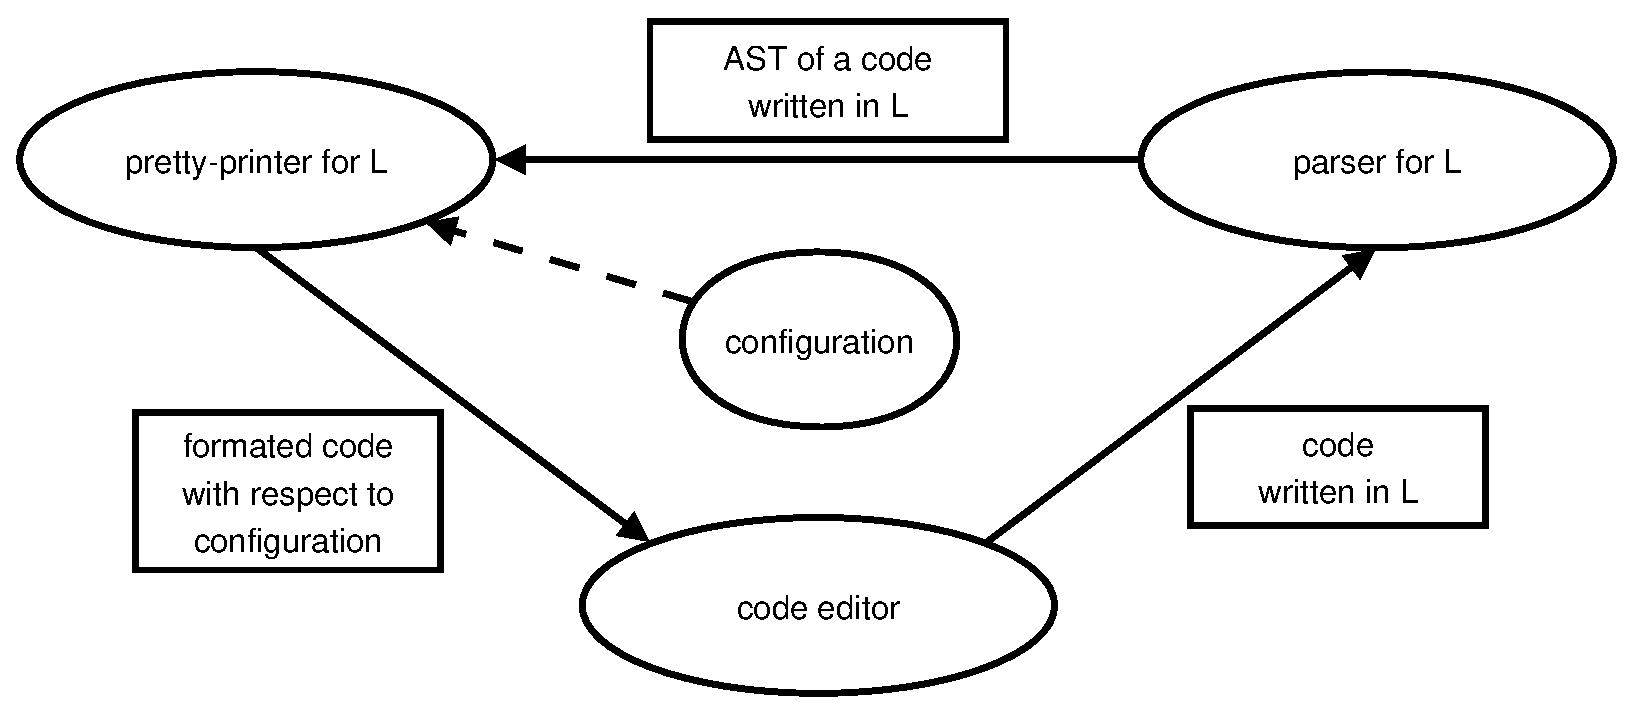
\includegraphics[scale=0.51]{pictures/PrettyPrinterPrinciple.eps}
\label{PrettyPrinterPrinciple}
\end{figure}
\noindent
\subsubsection {Ad-hoc Pretty Printer}
This kind of pretty printers is the best-known and the most widespread. These pretty printers are located in most current code editors or development environments intended for concrete imperative languages like \textsc{C}, \textsc{C++}, \textsc{Java}, \textsc{Pascal}, etc.  Each of them allows for formatting only the language to which the pretty printer is dedicated. The result of pretty-printing can be affected only by limited configurability. Settings of the pretty printer mostly offers only certain places with limited domain to change such as the definition of the character sequence for indenting, setting whether the left brace identifying the start of the method should be on the new line or be preceded by one whitespace, etc.

\subsubsection {Generic Pretty Printer}
This concept is the opposite of ad-hoc pretty printers. The correct generic pretty printer should be able to format an arbitrary number of languages and the options how to configure the formatting of a given language should be very wide. Nowadays, it is difficult to find some commercial projects, where this type of pretty printers were used. This concept is rather a matter of theoretical sphere and its realizations are mostly contained in research projects as a byproduct \cite{StrategoXT, PPML, Brand-Visser, DeJonge, OCaml}.

In order to  ensure that the generic pretty printer is able to format more languages which differ not only in details, the formatting rules determining a code appearance of a certain language have to be linked to some specification of a given language which is a grammar. The interconnection is performed in generic pretty printers through \textit{pretty-print tables} that contain formatting rules linked to rules of a grammar. This fact extends the possibilities to set up a code appearance in comparison with possibilities of ad-hoc pretty printers because the formatting rules can be easily changed, deleted or added. The pretty-print tables together with the AST of a given code further represent an input for the generic pretty-printer (see \cite{DeJonge} for details). The mentioned formatting rules may be obtained manually as well as may be generated from annotated grammar rules with the help of some heuristics (see \cite{DeJonge} for details). The following listing outlines what a pretty-print table can look like.

\newcommand{\mytrightarrow}{$\rightarrow$}
\newcommand{\mydash}{$-$}
\begin{expl}\label{PrettyPrintTable}
A sample of a pretty-print table published in \cite{DeJonge}. The table represents a mapping of grammar rules to corresponding formatting rules.  Grammar rules written in the \textsc{Syntax Definition Formalism (SDF)} \cite{SDF} are located  on the left side of dashes and further formatting rules are located on the right side. 
\begingroup
\fontsize{10pt}{12pt}
\begin{Verbatim}[commandchars=\\\{\}]
"package" Name ";" \mytrightarrow PackagedDeclaration \mydash
    H [KW["package"] H hs=0 [ 1 ";"]],
"import" Name ";" \mytrightarrow ImportDeclaration \mydash
    H [KW["import"] H hs=0 [ 1 ";"]],
"import" Name "." "*" ";" \mytrightarrow ImportDeclaration \mydash
    H [KW["import”] H hs=0 [ 1 "." "*" ";"]]
\end{Verbatim}
\endgroup
\end{expl}

The generic pretty printer brings advantages in high formatting configurability and possibilities to format more languages. Some generic pretty printers allow for formatting code into more formats specifying the same appearance of the code as for example plain text, \textsc{Latex} format or HTML. This feature is usually realized by division of the pretty-printer into a front-end and a back-end. The front-end of the pretty-printer is responsible for transforming pretty-print tables and AST into the intermediate language expressing a code formatting. Then the beck-end transforms the intermediate language into a given format specifying the appearance of a given code. Since the back-end of the pretty-printer in itself is not generic, a back-end has to exist for each format. A schema on the \textit{Figure \ref{GenericPrinterPrinciple}} reflects  information contained in this paragraph.

\begin{figure}[h!]
\centering
\caption{A schema of a generic pretty-printer with three back-ends.}
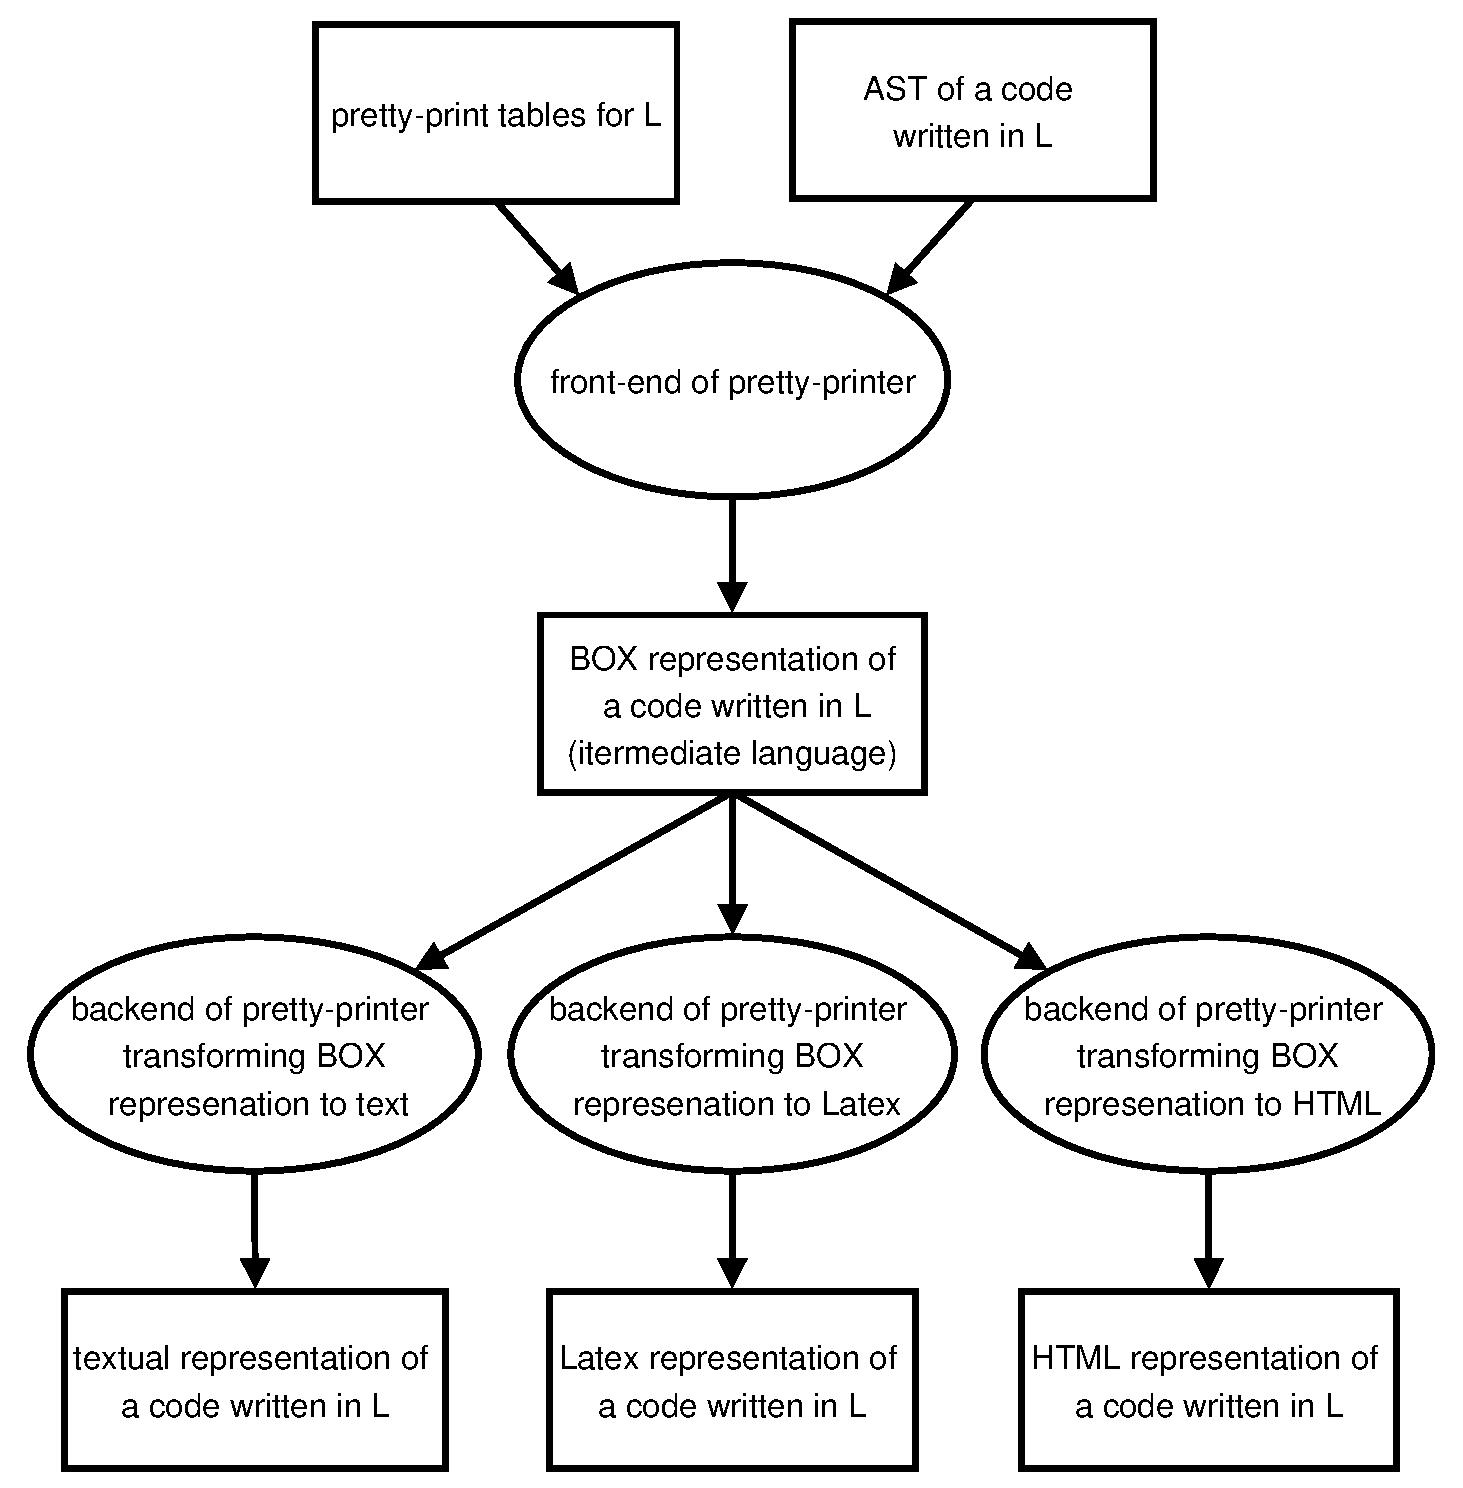
\includegraphics[scale=0.51]{pictures/GenericPrettyPrinter.eps}
\label{GenericPrinterPrinciple}
\end{figure}
\noindent
\section {Box Representation}

The concept using an intermediate language  was mentioned  in the previous paragraph. This intermediate language tends to be the \textit{box representation} which is a data structure formed from elements called \textit{boxes}.

\subsection{Box}

The box is a construction element of the box representation. This element can be either a string token related to some terminal rule of the grammar or a group of other elements among which vertical and horizontal relative positions or an indentation are defined  as it can be seen in the \textit{Figure \ref{BoxExample}}. This means that the box representation is also a composite box because the box representation is essentially a tree structure with regard to composing boxes.

\begin{figure}[h!]
\centering
\caption{An example of the box representation defining the appearance of the if statement from a C-based language.}
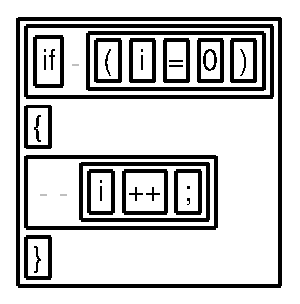
\includegraphics[scale=0.65]{pictures/BoxRepresentation.eps}
\label{BoxExample}
\end{figure}
\noindent

\subsection{Box Language}

Even though the box representation enables to define the appearance of a code written in some language, it is necessary to define what types of boxes will be used and how they will be assembled together. Therefore the box language serves for this purpose. The box language consists of operators that define creating of composite boxes. Each operator is related to a particular composite box type like a horizontal box, a vertical box or indenting box. The operators can be further configured using parameters which are reflected into corresponding composite boxes for example where it is possible to change spacing between inner boxes, a spacing character, etc. The mentioned operators are applied in formatting rules in pretty-print tables where usages of operators encapsulates keywords, calls of grammar rules and other usages of operators. The composition of operator's usages form a tree structure similarly like boxes in the box representation. The usages of operators can be seen in formatting rules on right sides in the \textit{Listing \ref{PrettyPrintTable}}. 

Since the concept of operators and their usages will be often mentioned in the remaining text, the following terminology is introduced.

\subsubsection {Box Model}

Since usages of operators of a box language serves as a pattern for the resulting box representation, a collection of formatting rules related to grammar rules of a particular language will be called a box model.

\subsubsection {Box Meta-model}

Since the types of operators and their parameters may be much more as well as the count of box languages, a set of operators and relevant parameters which can be used will be called a box meta-model. In other words, the box language will be referred to as a box meta-model.

\section {Existing Box Meta-models}
\label{ExistingBoxMetaModels}
This section contains a description of box meta-models that was published in papers or whose implementations are located in realized research projects. The concrete names and references of the mentioned papers and projects are mentioned bellow. The describing meta-models will be called by the name of a relevant project or by surnames of relevant paper's autors. 

\subsection {Stratego/XT}

The first describing meta-model is part of the \textsc{Stratego/XT} project~\cite{StrategoXT} of which the XT is a toolset for program transformation from one language to another and for other issues related to the meta-programming \cite{Metaprogramming}. Furthermore, the \textsc{Stratego} is a language providing rewriting rules for expressing basic transformations.

\subsubsection{Box Meta-model Description}

The source of the meta-model specifies the format of a textual usage as follows. The name of the operator stands at the first place and a usage of corresponding parameters follows after it. Finally, the boxes that are intended for formatting are placed at the end of this section and are enclosed in square brackets. This box meta-model is composed only from the following list of operators.

\begin{itemize}
\item \textbf{H} - The operator aligns boxes horizontally and also inserts spacing defined by the \textbf{hs} parameter between boxes. The \textbf{hs} parameter expresses a count of given characters which will be inserted.
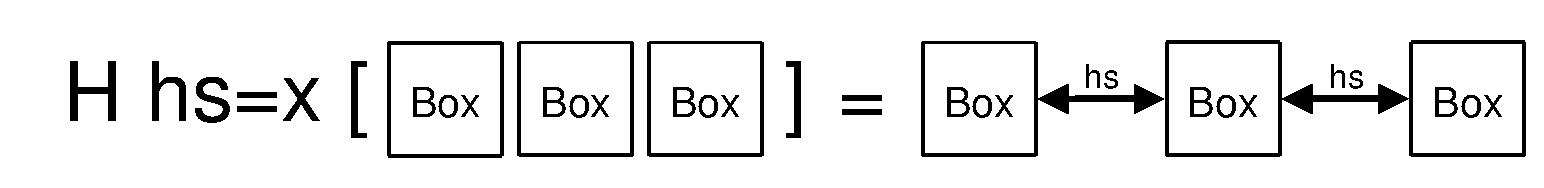
\includegraphics[scale=0.4]{pictures/StrategoXT-H.eps}
\item \textbf{V} - The operator aligns boxes vertically and inserts spacing defined by the \textbf{vs} parameter between boxes. The \textbf{vs} parameter expresses a count of new lines which will be inserted. The operator has also the second parameter \textbf{is} that allows for setting indentation between the first box and the others. The \textbf{is} parameter expresses a count of inserted characters as well as the \textbf{hs} parameter of the \textbf{H} operator.
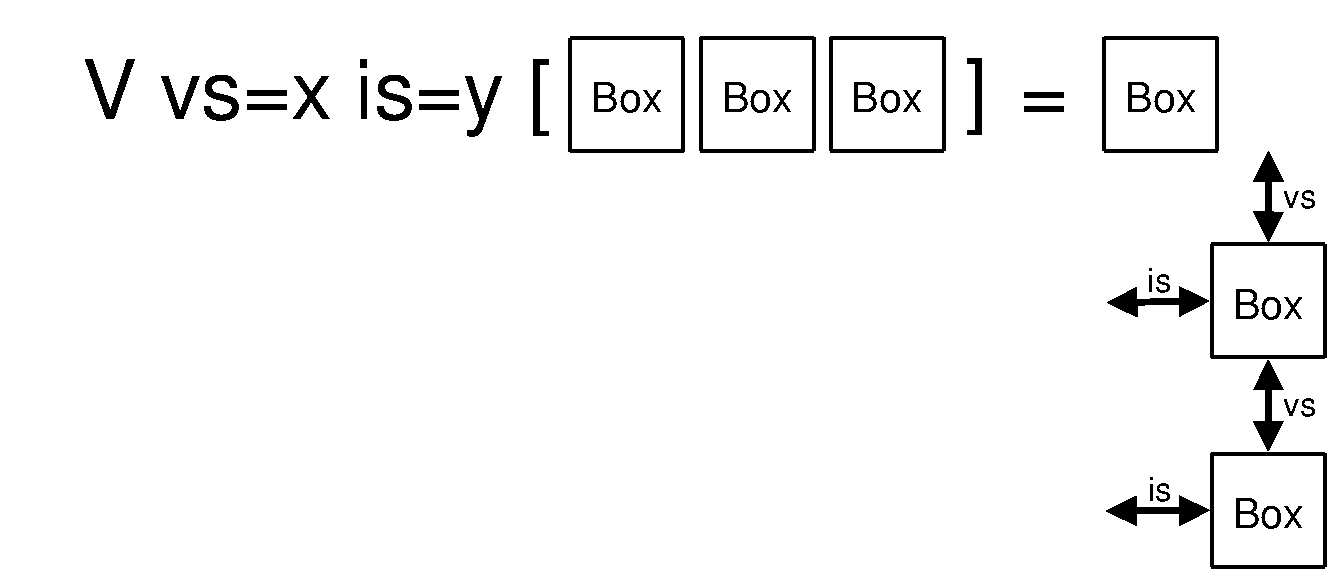
\includegraphics[scale=0.4]{pictures/StrategoXT-V.eps}
\item \textbf{A} - The operator aligns boxes into a table and further two numeric parameters \textbf{hs} and \textbf{vs}, which are equivalent to parameters of the operators \textbf{H} and \textbf{V}, belong to it. Although, the \textbf{A} operator defines that a particular group of boxes will be encased into a table, it is necessary to define in which columns and rows  boxes will be placed. Therefore the subsidiary operator \textbf{R}  serves for this purpose.
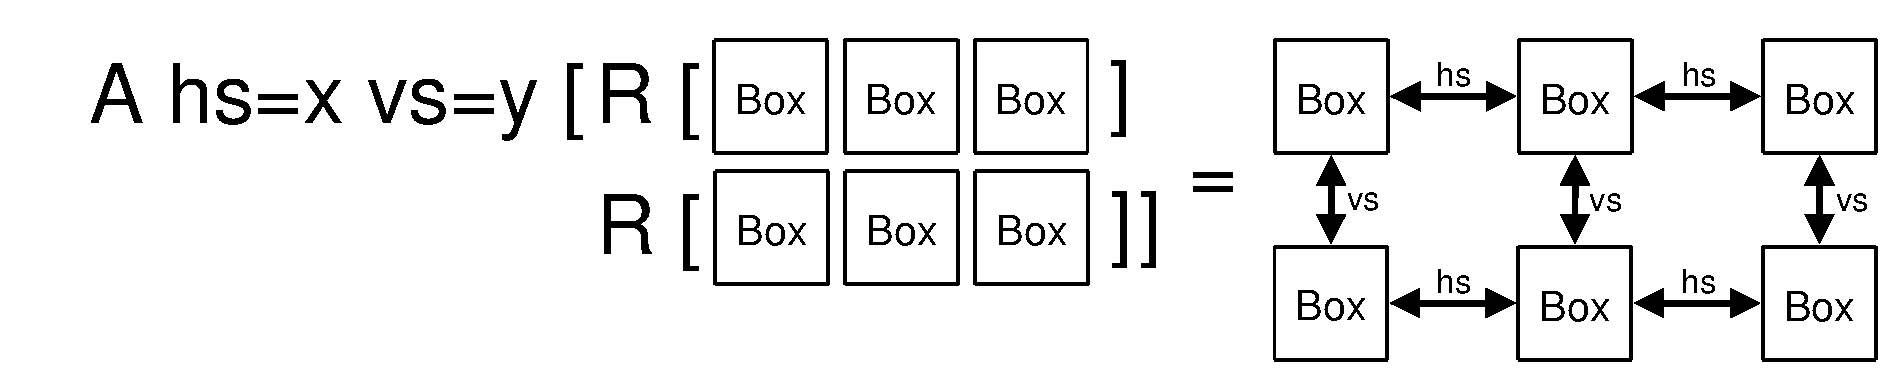
\includegraphics[scale=0.4]{pictures/StrategoXT-A.eps}
\item \textbf{R} - This subsidiary operator allows for defining rows of a table. Boxes that are inside of the same operator are on the same row of a table and also boxes that are at the same position inside of the operators \textbf{R} are in the same column of a table.
\end{itemize}

\subsection {PPML}

The next meta-model is integrated into the PPML \cite{PPML} formalism, whose full name is \textsc{Pretty Printer Meta Language}. The PPML has been used in the \textsc{Centaur} system \cite{Centaur} to write pretty printers for various programming languages.

\subsubsection{Box Meta-model Description}

The PPML formalism encloses the textual usage of a meta-model into square brackets. Furthermore, the name of a used operator and a usage of corresponding operators are enclosed in angle brackets. The boxes waiting for be formatting follows after the definition in angle brackets. The box meta-model is comprised of four following operators.

\begin{itemize}
\item \textbf{H} - The operator aligns boxes horizontally and inserts spacing defined by the \textbf{dx} parameter between boxes. The \textbf{dx} parameter expresses a count of given characters which will be inserted.
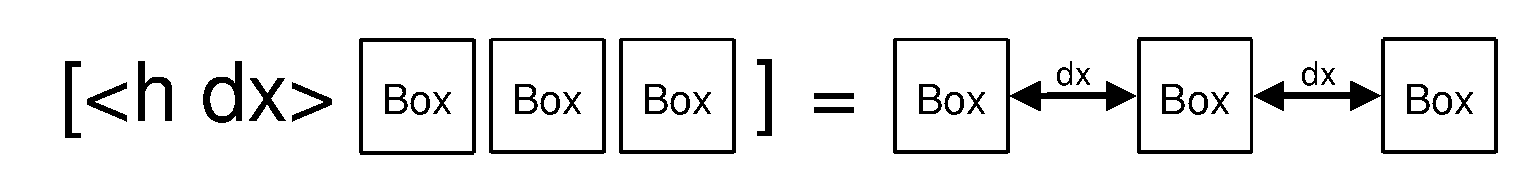
\includegraphics[scale=0.4]{pictures/PPML-H.eps}
\item \textbf{V} - The operator aligns boxes vertically and inserts spacing defined by the \textbf{dy} parameter between boxes. The \textbf{dy} parameter expresses a count of new lines which will be inserted. The operator has also the second  parameter \textbf{i} that allows for setting indentation of the second box. Although, the source of the meta-model does not mention indentation of other lines,  it results from descriptions of following operators.
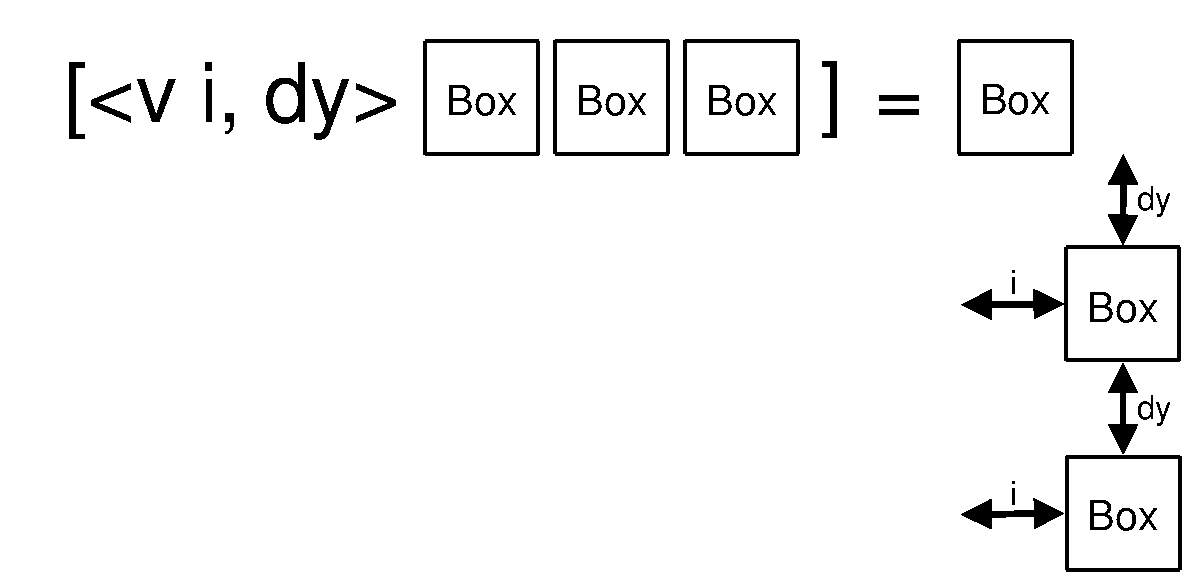
\includegraphics[scale=0.4]{pictures/PPML-V.eps}
\item \textbf{HV} - The operator aligns boxes as follows. The result formatting depends on whether the total length of boxes including horizontal spacing exceeds the maximal length of line, which is fixed. When the length of all boxes including horizontal spacing is smaller than the maximum length of line, then the boxes are aligned horizontally with spacing defined in the \textbf{dx} parameter. Otherwise, the first line is filled as much as possible and the second one is indented of count of spacing character, which is defined in the \textbf{i} parameter. The operator fills the second line like for the first and the following lines are vertically aligned with the second line. Two consecutive lines are separated by blank lines, whose count is defined in the \textbf{dy} parameter.
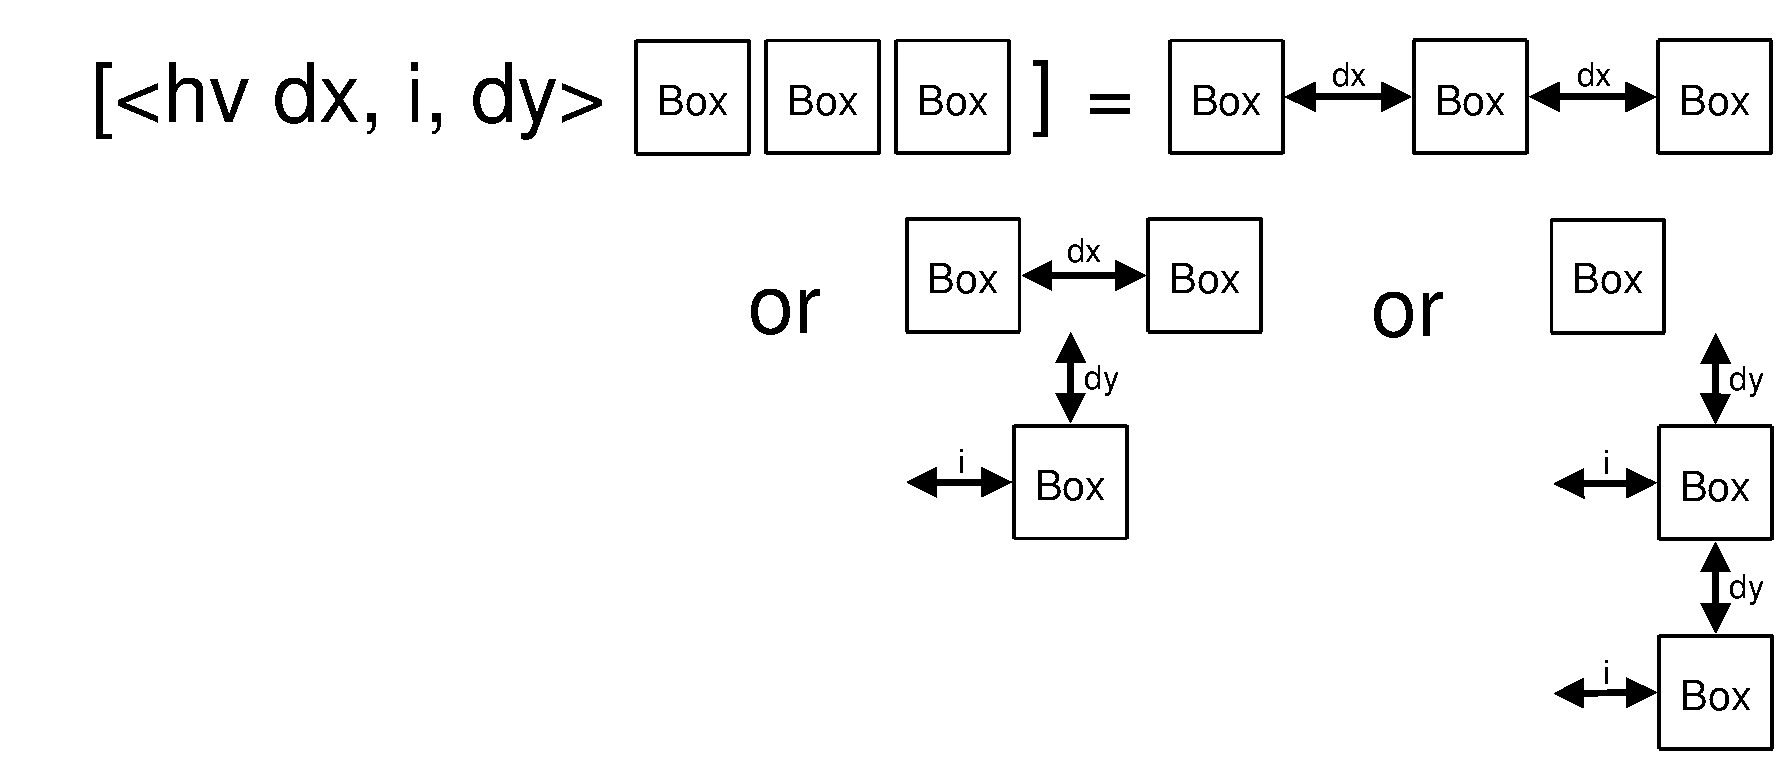
\includegraphics[scale=0.4]{pictures/PPML-HV.eps}
\item \textbf{HOV} - The operator behaves like the operator \textbf{H} when the total length of boxes including horizontal spacing does not exceed the maximal line length. Otherwise, the operator behaves like the operator \textbf{V}. The parameters of the operator have the same significance as with the previous operators.
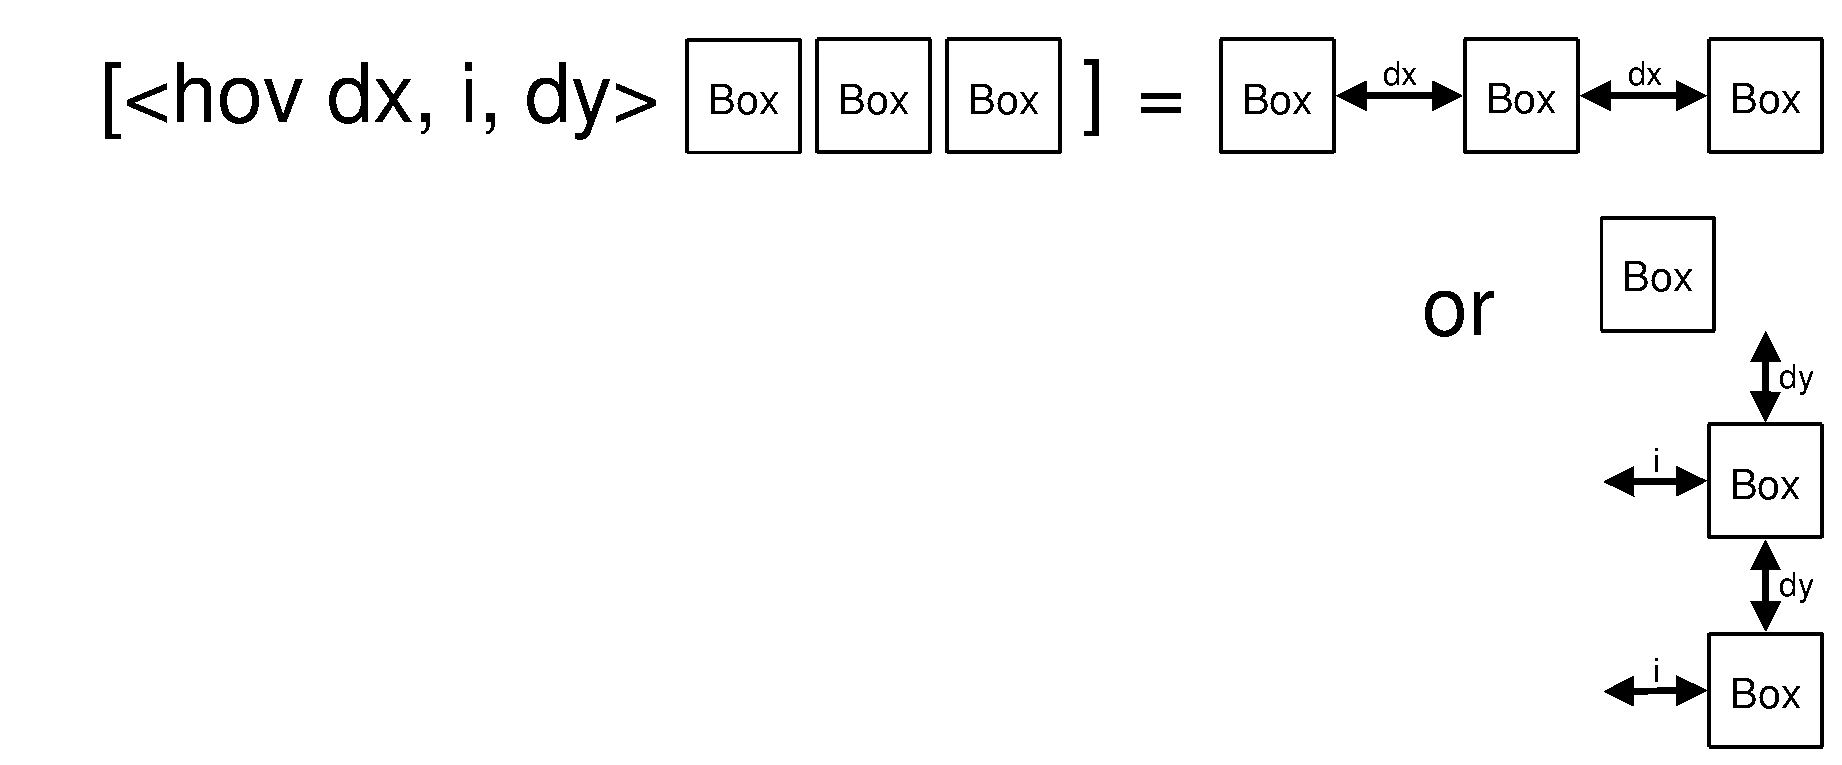
\includegraphics[scale=0.4]{pictures/PPML-HOV.eps}
\end{itemize}

\subsection {Brand-Visser}

The next meta-model was published in the \textit{"Generation of Formatters for Context Free Languages"} paper \cite{Brand-Visser} written  by Mark van den Brand and Eelco Visser. The paper deals with the theory of generic pretty printers. The purpose of pretty printers and theirs relationship with a grammar is formally explained in the paper. The paper also includes considerations on the division of generic pretty printers into front-ends and back-ends with use of the box representation as an intermediate language. 

\subsubsection{Box Meta-model Description}

The paper defines the same syntax for textual usages of operators as was introduced with the \textsc{Stratego/XT} box meta-model and also there are some same operators with the same corresponding parameters. The operators were mentioned that defines relative positions between boxes in previous box meta-models. This box meta-model brings another kind of operators, where operators do not define positions but determine what font and font parameters will be associated with the text of input boxes. The meta-model contains the following list of positional and non-positional operators.

\subsubsection{Positional Operators}
\begin{itemize}
\item \textbf{H} - The operator aligns inner boxes horizontally exactly like the \textbf{H} operator from the \textsc{Stratego/XT} box meta-model.  The \textbf{hs} parameter also belongs to the operator with the same functionality.
\item \textbf{V} - The operator aligns inner boxes vertically exactly like the \textbf{V} operator from the \textsc{Stratego/XT} box meta-model with an exception that the operator does not indent the second and other boxes against the first.  The parameter \textbf{vs} belongs to the operator with the same functionality.
\item \textbf{HV} -  The operator aligns boxes as follows. The result formatting depends on whether the total length of boxes including horizontal spacing exceeds the maximal length of line, which is fixed. When the length of all boxes including horizontal spacing is smaller than the maximum length of line, then the boxes are aligned horizontally with spacing defined in the \textbf{hs} parameter. Otherwise, the first line is filled as much as possible and the rest of the boxes is filled into the second line appying the same rule as for the first line. Two consecutive lines are separated by blank lines, whose count is defined in the \textbf{vs}  parameter.
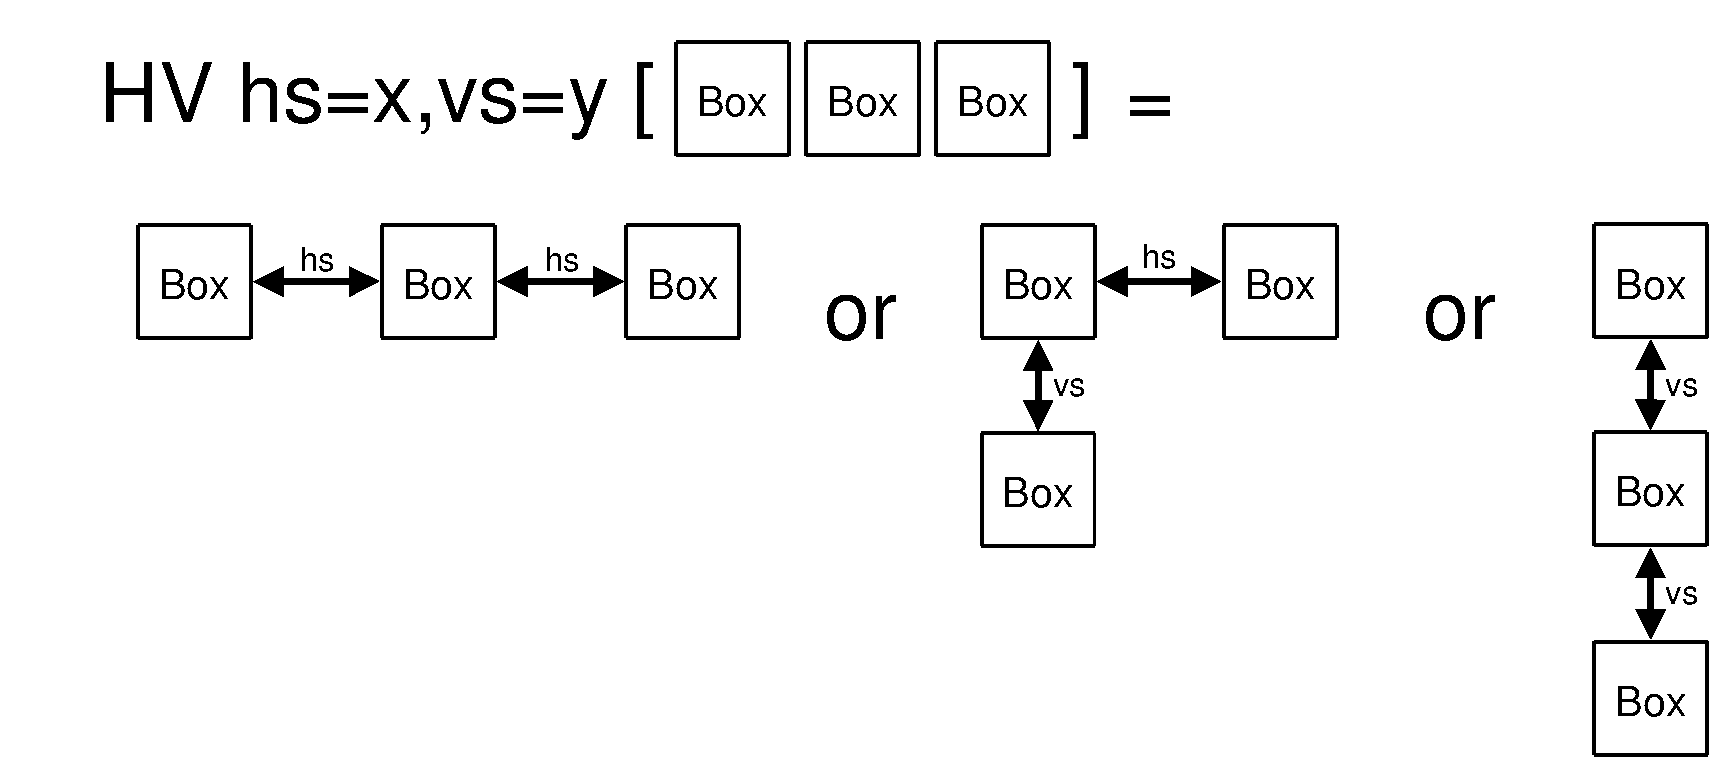
\includegraphics[scale=0.4]{pictures/Brand-Visser-HV.eps}
\item \textbf{HOV} - The operator behaves like the operator \textbf{H} when the total length of boxes including horizontal spacing does not exceed the maximal line length. Otherwise, the operator behaves like the \textbf{V} operator. The parameters of the operator have the same significance as with the previous operators.
\item \textbf{I} - The parameter increases the indentation of inner boxes by the value defined in the \textbf{is} parameter. The indentation is applied when the box is vertically aligned against some other boxes. In other words, the operator has its effect when it is contained in another operator with vertical alignment as an inner box.
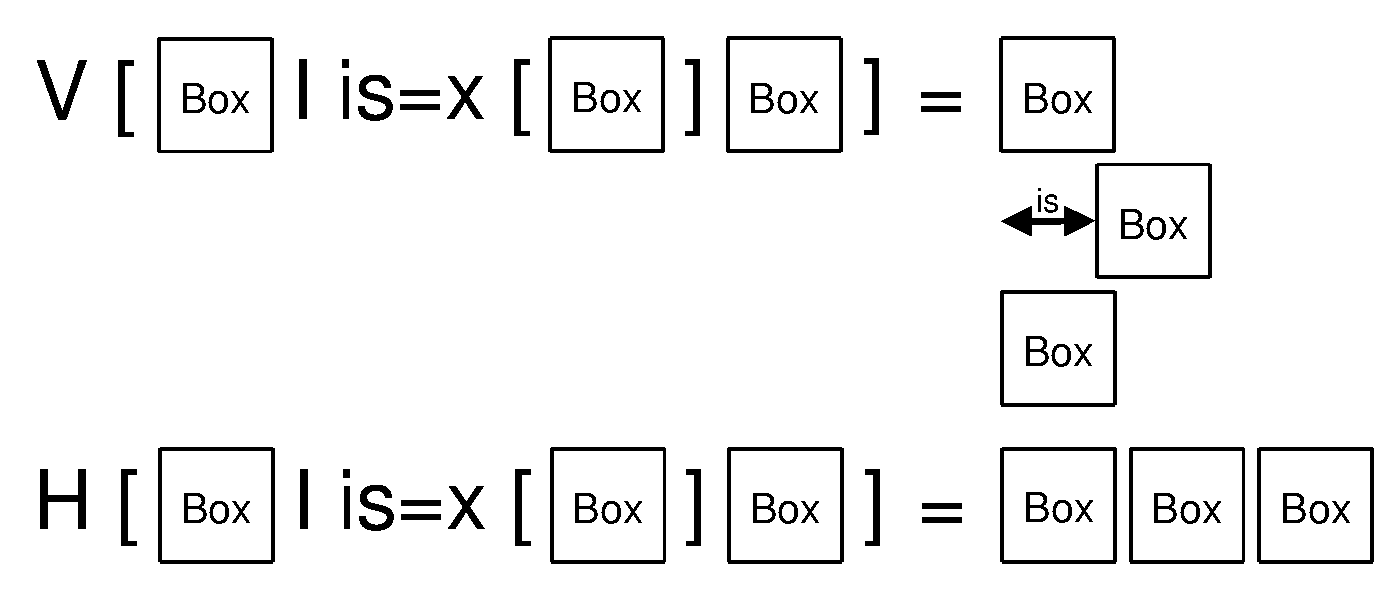
\includegraphics[scale=0.4]{pictures/Brand-Visser-I.eps}
\item \textbf{WD} - The operator translates inner boxes into an empty boxes with dimensions equal to those of inner boxes.
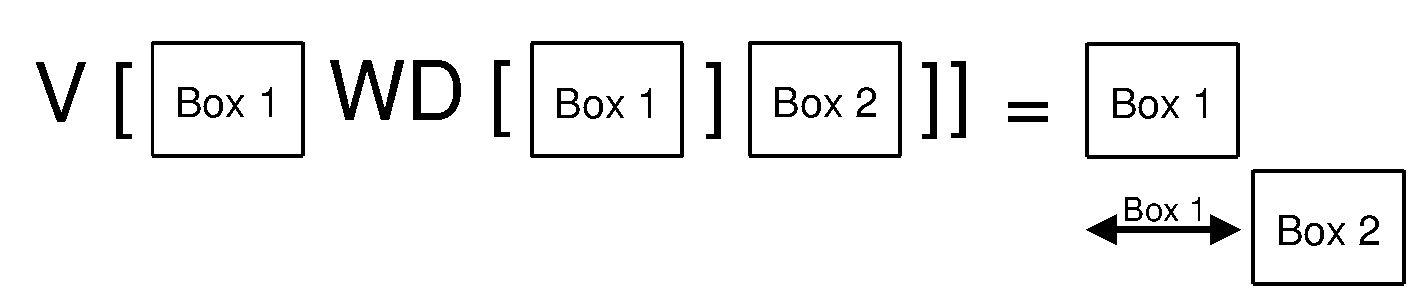
\includegraphics[scale=0.4]{pictures/Brand-Visser-WD.eps}
\item \textbf{A} - The operator aligns inner boxes into a table exactly like the \textbf{A} operator from the \textsc{Stratego/XT} box meta-model. The operator also exploits the operator \textbf{R} in order to define rows of the table and it is also tied with the parameters \textbf{hs}, \textbf{vs} and \textbf{is}, which perform the same function like in the \textsc{Stratego/XT} box meta-model. This version of the operators \textbf{A} additionally provides possibility to align columns to left, center or right by signs \textbf{l}, \textbf{c}, \textbf{r} enclosed in parentheses. The parentheses should enclose the same number of signs as is the number of columns. In other words, each column should have a sign expressing its alignment.
\item \textbf{R} - This operator serves as subsidiary operator for the \textbf{A} operator. The operator \textbf{R} defines rows of a table exactly like in the \textbf{Stratego/XT} box meta-model. 
\end{itemize}

\subsubsection{Non-positional Operators}
\begin{itemize}
\item \textbf{F} - The operator is dedicated to specify a font configuration. and associate it with the text of inner boxes. The font configuration can be defined by the operator \textbf{fn} specifying a font name, \textbf{fm} specifying a font family, \textbf{se} specifying font series, \textbf{sh} specifying a font shape, \textbf{sz} specifying a font size and \textbf{cl} specifying a font color. 
\item \textbf{KW} - The operator associates a font indicating keywords with the text of inner boxes. 
\item \textbf{VAR} - The operator associates a font indicating variables with the text of inner boxes. 
\item \textbf{NUM} - The operator associates a font indicating numbers with the text of inner boxes. 
\item \textbf{MATH} - The operator associates a font indicating mathematical symbols with the text of inner boxes. 
\item \textbf{COMM} - The operator associates a font indicating comments with the text of inner boxes. 
\item \textbf{ESC} - The operator represents an escape mechanism to obtain special symbols in the formatted text.
\end{itemize}

\subsection {DeJonge}

Firstly, the next box meta-model was published in the \textit{"A Pretty Printer for Every Occasion"} paper \cite{DeJonge} written by Merijn de Jonge and after its definition was refined in author's doctoral thesis \cite{DeJongePhD}.  The paper and doctoral thesis deal with the theory of generic pretty printers similarly like the source of the previous box meta-model. The paper also deals with an application of the theory where the subject is to nicely pretty-print input data stored in XML.

\subsubsection{Box Meta-model Description}

As M. de Jonge refers to the \textsc{Stratego/XT} project and the paper written by M. van den Brand and E. Visser, which were mentioned above, some similarities with the \textsc{Stratego/XT} and \textsc{Brand-Visser} box meta-models can be found. The syntax of a textual usage of a box meta-model is the same like in the other two box meta-models. Several of the same operators and its parameters are contained in this meta-model. 
\vspace{0.5cm}

\subsubsection{Positional Operators}
\begin{itemize}
\item \textbf{H} - The operator aligns inner boxes horizontally exactly like the \textbf{H} operator from the \textsc{Stratego/XT} and \textsc{Brand-Visser} box meta-model.  The \textbf{hs} parameter also belongs to the operator with the same functionality.
\item \textbf{V} - The operator aligns inner boxes vertically exactly like the \textbf{V} operator from the \textsc{Stratego/XT} and \textsc{Brand-Visser} box meta-model.  The parameters \textbf{vs} and \textbf{is} also belongs to the operator with the same functionality.
\item \textbf{HV} -  The operator aligns boxes as the same operator from the \textsc{Brand-Visser} box meta-model. The parameters \textbf{hs} and \textbf{vs} also belong to the operator with the same functionality. The operator has one extra parameter \textbf{is} for indentation of the second and next lines against the first as with the \textbf{V} operator.
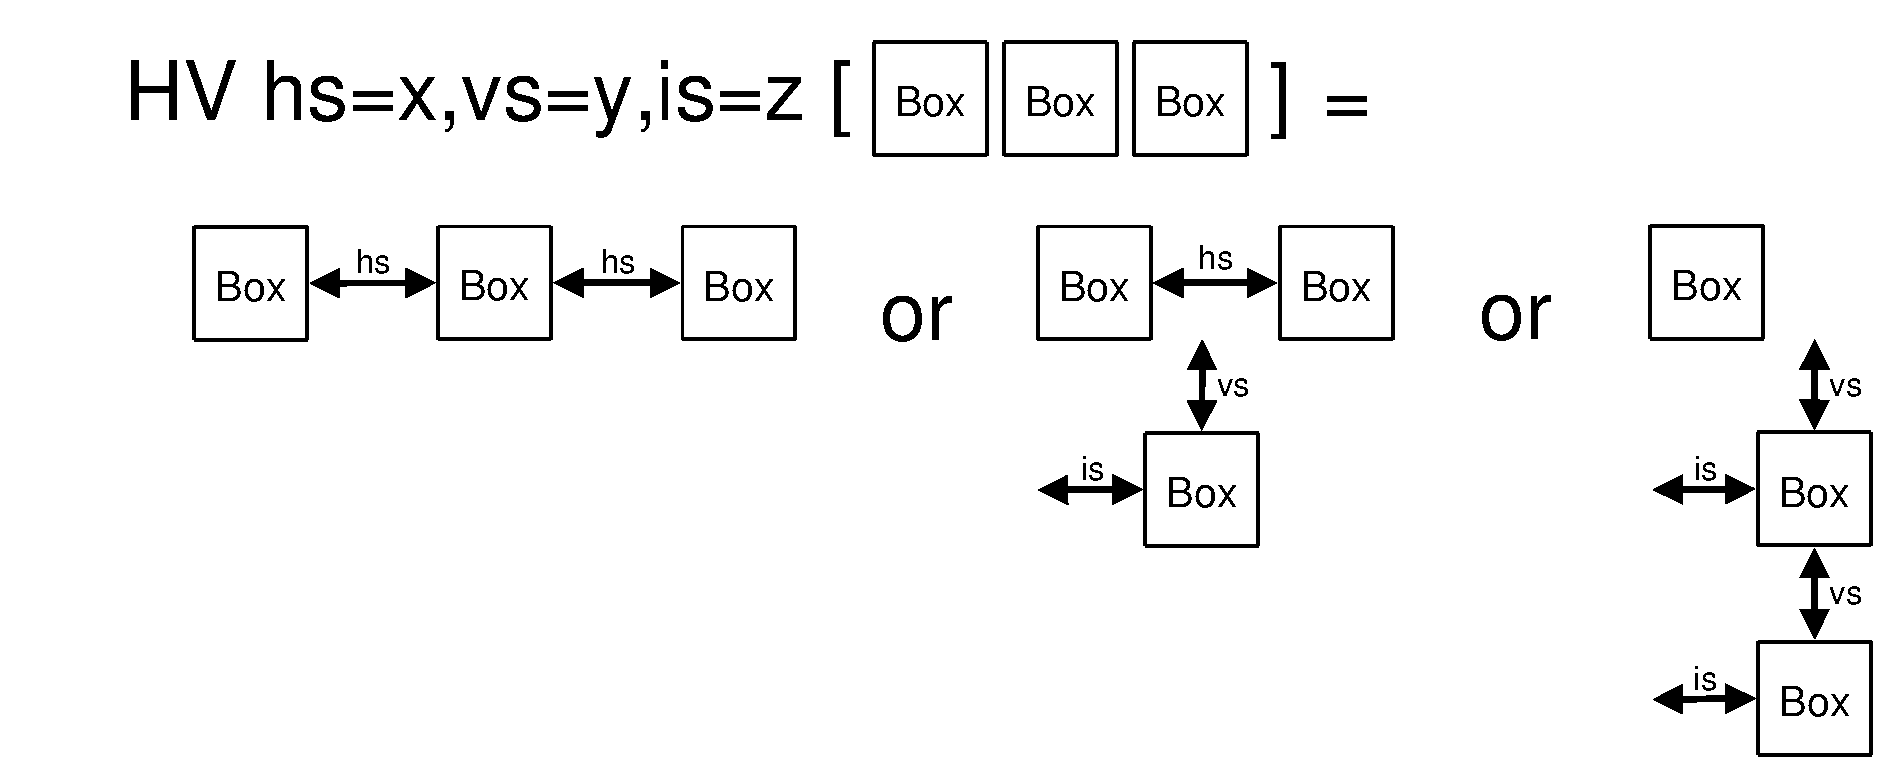
\includegraphics[scale=0.4]{pictures/DeJonge-HV.eps}
\item \textbf{A} - The operator aligns inner boxes into a table exactly like the \textbf{A} operator from the \textsc{Stratego/XT} box meta-model. The operator also exploits the \textbf{R} operator in order to define rows of the table and it is also tied with the parameters \textbf{hs}, \textbf{vs} and \textbf{is}, which perform the same function like in the \textsc{Stratego/XT} box meta-model.
\item \textbf{R} - This operator serves as subsidiary operator for the \textbf{A} operator. The \textbf{R} operator  defines rows of a table exactly like in the \textsc{Stratego/XT} box meta-model. 
\item \textbf{ALT} - The operator represents a generalization of the operator \textbf{HOV} known from the \textsc{Brand-Visser} box meta-model. The \textbf{HOV} operator aligns boxes horizontally or vertically according to whether the horizontally alignment does not exceed the maximum line size; the \textbf{ALT} operator uses the first inner box as a result when the first inner box does not exceed the maximum line size, otherwise the operator similarly uses a next inner box under the same condition. If the box is last in a sequence of inner boxes, the box does not have to satisfy the condition in order to be used. Thus the identical behavior of the \textbf{HOV} operator can be replaced by using the \textbf{ALT} operator  and by using the operators \textbf{H} and \textbf{V} that represent the first and the second inner boxes. Furthermore, the inner operators have to have the same inner boxes.
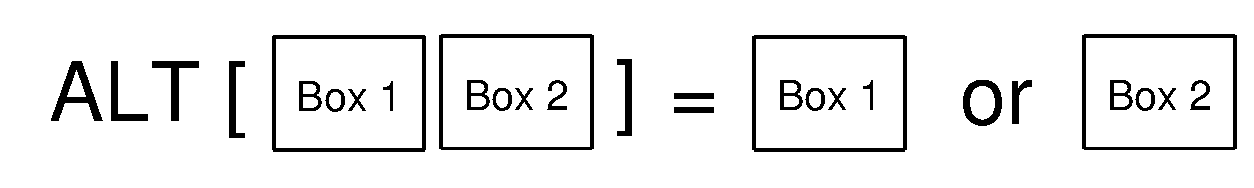
\includegraphics[scale=0.4]{pictures/DeJonge-ALT.eps}
\end{itemize}

\subsubsection{Non-positional Operators}
\begin{itemize}
\item \textbf{F} - The operator is dedicated to specify a font configuration. The specified font configuration are further associated with the text of inner boxes.
\item \textbf{KW} - The operator associates a font indicating keywords with the text of inner boxes. 
\item \textbf{VAR} - The operator associates a font indicating variables with the text of inner boxes. 
\item \textbf{NUM} - The operator associates a font indicating numbers with the text of inner boxes. 
\item \textbf{MATH} - The operator associates a font indicating mathematical symbols with the text of inner boxes. 
\item \textbf{LBL} - The operator serves to define a label for inner boxes. 
\item \textbf{REF} - The operator serves to refer to a labeled box.
\item \textbf{C} - The operator serves to represent lines of code and format them.
\end{itemize}

\subsection {Format Module for OCaml}

The last meta-model is present in a pretty-printing engine provided by the \textsc{Format} module of standard libraries of the \textsc{OCaml} system which is the main implementation of the general-purpose programming language \textsc{Caml} supporting functional, imperative, and object-oriented programming styles.

\subsubsection{Box Meta-model Description}
Since the source of this box meta-model conceives operator as a function of a programming language transforming one character sequence to another, the box meta-model does not have any textual usage of operators known from the previous descriptions of box meta-models. The source also defines overall formatting differently. The elementary inner boxes are represented by corresponding text directly and further they are separated by a \textit{special break}. All texts of boxes together with special breaks represent an input character sequence for an operator which subsequently transforms. After the character sequence is transformed by all necessary operators, the special breaks are replaced by white characters ensuring indentation, horizontal or vertical spacing. The function performing this action knows exactly whether to indent or make same spacing gaps on the position of a special break in the input character sequence. Since indentation and spacing are solved globally, the operators do not hold any parameters. The following list of operators is part of this box meta-model. Just to clarify, the "-" means an arbitrary character and the "b" represents a special break in the following description.
\begin{itemize}
\item \textbf{H} - The operator aligns inner boxes horizontally similarly like the \textbf{H} operators from the previous box meta-models. The operator preserves the input character sequence and does not wrap it.
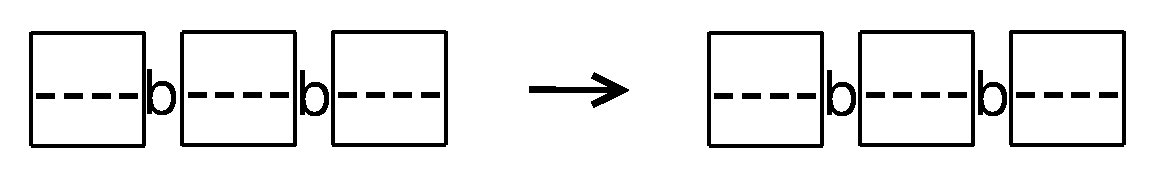
\includegraphics[scale=0.4]{pictures/OCaml-H.eps}
\item \textbf{V} - The operator aligns inner boxes horizontally similarly like the \textbf{V} operators from the previous box meta-models. The operator wraps the input character sequence after each  occurrence of a special break.
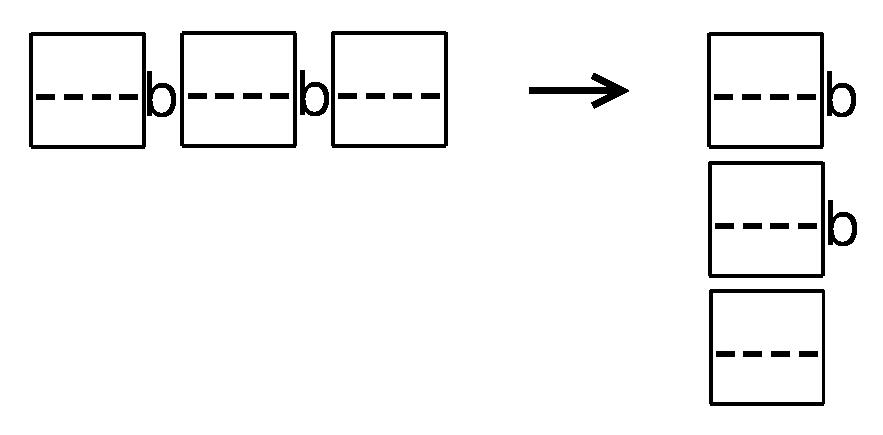
\includegraphics[scale=0.4]{pictures/OCaml-V.eps}
\item \textbf{HOV} - The operator aligns inner boxes like the \textbf{HV} operators from the previous box meta-models. The functionalities of the operators \textbf{HV} and \textbf{HOV} are swapped in this box meta-model. The operator fills the first line gradually by the inner boxes from the character sequence until an additional box together with a following special break fit into the line. In case it does not fit, the box together with a special break is added into the next line.
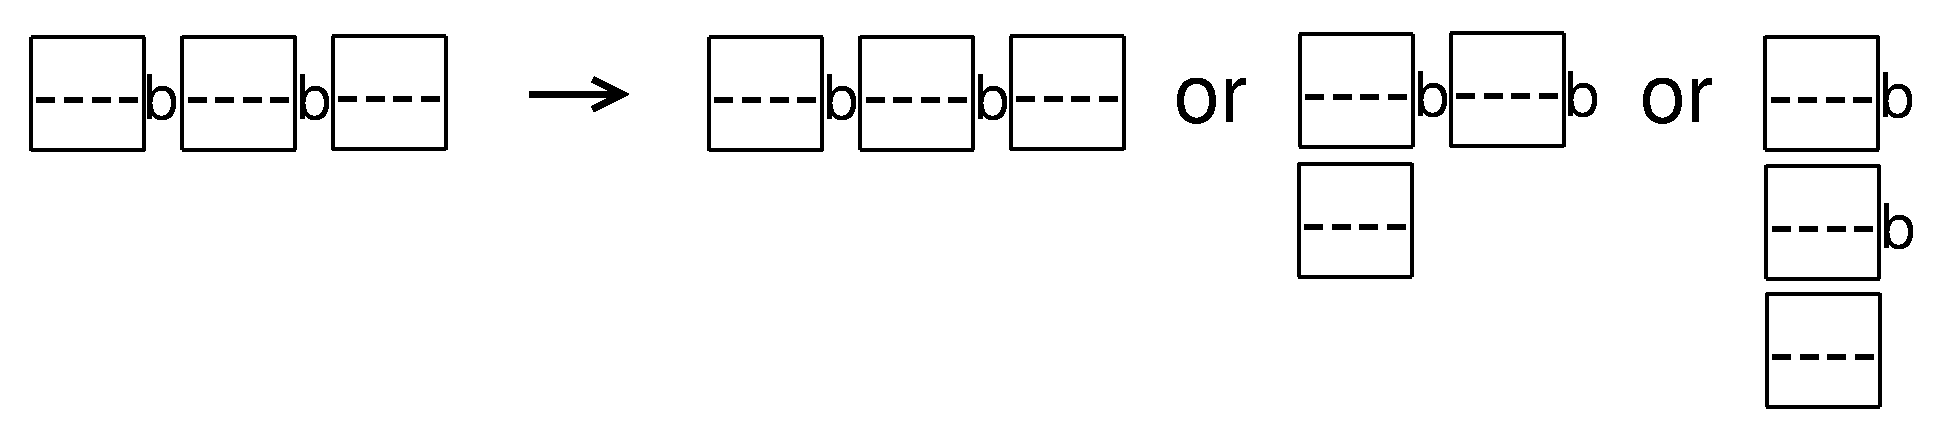
\includegraphics[scale=0.4]{pictures/OCaml-HOV.eps}
\item \textbf{HV} - The operator aligns inner boxes like the \textbf{HOV} operators from the previous box meta-models. The functionalities of the operators \textbf{HV} and \textbf{HOV} are swapped in this box meta-model. The operator formats the character sequence like the \textbf{H} operator when the length of the sequence does not exceed maximum line size. Otherwise, it works like the \textbf{V} operator. \newpage
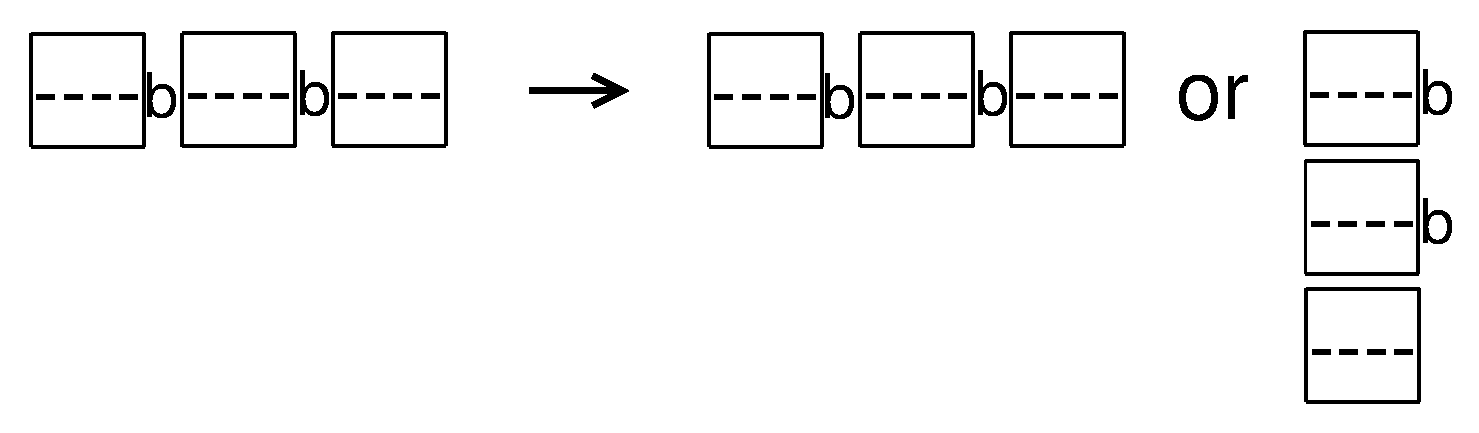
\includegraphics[scale=0.4]{pictures/OCaml-HV.eps}

\end{itemize}

\subsection{Summary}
\label{IdealMetaModel}
Five already existing box meta-models  were introduced and described in the text above. This is enough information to design box meta-model that meets all requirements for code formatting. Definitely, it would be good to keep the syntax of a textual usages of operators that was used for operators of most box meta-models, specially the \textsc{Stratego/XT}, \textsc{DeJonge} and \textsc{Brand-Visser} box meta-model because this may act as informal standard.

Even though common positional operators will meet all requirements for defining relative positions among inner boxes, it would be beneficial to include also non-positional operators in this box meta-model. The operators that associate font configurations with text of inner boxes could be a good tool for defining syntax highlighting for a particular language and will be called \textit{highlight operators} in the following text. The question is how to deal with comments. When the comments are realized by special tokens in the \textsc{Xtext} framework, highlight operators can be used for differentiation of this text kind because the token can be expressed by some box from the perspective of the box representation as it was realized in the \textsc{DeJonge} or \textsc{Brand-Visser} box meta-model. Still another problem to be solved is how how to wrap or variously format these comments that are represented by one elementary box. One way may be to introduce new kind of operators that would be able to modify text of inner boxes. This kind will be called \textit{transforming operators} in the following text.

In general, it is not difficult to invent many operators that  have  different formatting effects, but a box meta-model with high amount of operators would lose clarity and easy usability. Therefore the operators should be as general as possible. The following list of operators suggests what  the mentioned box meta-model may look like.  

\subsubsection{Positional Operators}
\begin{itemize}
\item \textbf{I} - Since this operator known from the \textsc{Brand-Visser} box meta-model allows for indenting a box individually in comparison with the indent parameter of vertical operators so this operator is a more general variant of indentation. The parameters \textbf{is} and \textbf{ic} would suit the operator. The \textbf{is} parameter expresses a number of characters needed to indentation and the \textbf{ic} parameter specifies indenting character.
\item \textbf{H} - The operator, which was contained in all mentioned box meta-models, aligns inner boxes horizontally and the parameters \textbf{hs} and \textbf{hc} are related to it. The \textbf{hs} parameter defines a number of characters forming a spacing gap and the \textbf{hc} parameter specifies a spacing character.
\item \textbf{V} -  The operator, which was contained in all mentioned box meta-models, aligns inner boxes vertically and the \textbf{vs} parameter defining a number of blank spacing lines is related to it.
\item \textbf{HV}- The operator known from the \textsc{DeJonge} and \textsc{Brand-Visser} box meta-model fills the first line by inner boxes and if there is no space left, it fills the next line. The parameters \textbf{hs}, \textbf{hc}, and \textbf{vs} are related to the operator and have the same functionalities like with the \textbf{H} and \textbf{V} operators. Newly, the \textbf{rs} parameter specifying maximum line size is present.
\item \textbf{ALT} - Since this operator is more general than the \textbf{HOV} operator,  only this operator is present in the box meta-model. Reasons why is the \textbf{ALT} operator more general are discussed in the description of the \textsc{DeJonge} box meta-model, from which the \textbf{ALT} operator comes. The operator uses the first inner box as a result when the length of the box does not exceed maximum line size specified by the \textbf{rs} parameter. Otherwise, the operator uses the next inner box.
\item \textbf{A} - The operator known from the \textsc{Stratego/XT}, \textsc{Brand-Visser} and \textsc{DeJonge} box meta-models aligns inner boxes into a table. The parameters \textbf{hs}, \textbf{hc}, and \textbf{vs} are related to the operator and have the same functionalities like with the \textbf{H} and \textbf{V} operators. Newly, the \textbf{ca} parameter specifying alignment of columns is present  as it was mentioned in the description of the \textsc{Brand-Visser} box meta-model.
\item \textbf{R} - The operator defines a row of a table specified by the \textbf{A} operator.
\item \textbf{WD} - The operator coming from the \textsc{Brand-Visser} box meta-model that translates inner boxes into an empty boxes with the same size.
\end{itemize}

\subsubsection{Highlight Operators}
\begin{itemize}
\item \textbf{F} - The operator known from the \textsc{Brand-Visser} and \textsc{DeJonge} box meta-models associates the text of inner boxes with a font configuration. The font configuration can be defined by the operator \textbf{f} specifying a font name, \textbf{w} specifying a font width, \textbf{i} specifying a font shape, \textbf{h} specifying a font size, \textbf{c} specifying a font color and \textbf{b} specifying a font background color. Since the operator is the most general from all highlight operators of both mentioned box meta-models and can supply them, it is not necessary to involve another highlight operators to this box meta-model.
\end{itemize} 

\subsubsection{Transforming Operators}
\begin{itemize}
\item \textbf{SL} - The operator formats single line comments. If the maximum line size specified by the \textbf{rs} parameter is exceeded by the length of the comment, the comment is properly splitted. Furthermore, the  \textbf{bs} parameter specifying a character sequence that denotes the begin of the comment belongs to the operator. 
\item \textbf{ML} - The operator formats multi line comments. If the maximum line size specified by the \textbf{rs} parameter is exceeded by the length of a line containing the comment, than the comment is properly splitted. The following  parameters belong to the operator. The parameters \textbf{bs} and \textbf{es} specify character sequences that denotes the begin and the end of the comment. And further the \textbf{is} parameter defines a character sequence serving for indentation of inner lines together with the last line of the comment.
\end{itemize}

\chapter{Goals Revisited}
\label{GoalsRevisited}
Contemporary concepts of code formatting and syntax highlighting for the \textsc{Xtext} framework is introduced in the \textit{Section \ref{CodeFormatting}} and the \textit{Section \ref{SyntaxHighlighting}}. Based on the previous text, it is obvious that the ways allowing for realizing these concepts are too user-demanding. The user has to know a part of the \textsc{Xtext} framework's internals and write a lot of \textsc{Java} code from scratch. Furthermore, for other users is difficult to distinguish how a given code exactly works at first glance.

The possibility to make code specifying a configuration of the pretty printer more readable and reduce quantity of code is to express a configuration of the pretty printer declaratively. The suitable candidate for this purpose is a configuration expressed as a box model. This expression tool discussed in the previous chapter is tried and tested on existing projects and it is a typical example of DSL. In essence, the pretty printer exploiting this expression mechanism is driven by a model parsed from the mentioned DSL. Moreover, the box meta-model allowing for defining diverse requirements on code formatting and syntax highlighting is designed in the \textit{Section \ref{IdealMetaModel}}. Hence the meta-model should serve as a template for directing models.

The previous chapter discusses that formatting rules (usages of operators) are linked to elements specifying the grammar rules, the DSL has to be designed so that its formatting rules are able to link to elements of rules of the Xtext's grammar.  Furthermore, it would be beneficial that the DSL has a similar syntax like the syntax designed for usage of operators contained in the ideal box meta-models because the syntax is often used with box meta-models of existing generic pretty-printers.

Although, the ideal box meta-model is designed with respect to widest formatting possibilities and generality of operators,  each user has own habits and requirements on the ideal meta-model. Thus the meta-model should be extensible in order for the user to be allowed to add another operator into the box meta-model. As the declarative way is more comfortable compared to many lines of code in a common imperative programming language,a DSL allowing for specifying a box meta-model  should be created. The language should allow for defining operators with corresponding parameters and interconnect operators with specifications of behavior that have to be specified in an imperative language due to the complexity. 

The DSL should be able to capture the requirements on code formatting and syntax highlighting by formatting rules. The formatting rules have to be somehow reflected to internals of the \textsc{Xtext} framework dealing with these two concepts. Two solutions are offered at the first glance. The first one is to generate a code of the internals from the directing model and the second one is to make an interpreter of a model that would be connected to the internals. The next goal will be to consider which solution would be better and make a prototype of the better one.

Although, the formatting configuration of generic pretty printer expressed through a DSL makes work easier but still the user has to create a formatting configuration from scratch. Thus the next goal is to examine whether it is possible to create some heuristics allowing for generating an initial formatting configuration based on the knowledge of a particular grammar.  Subsequently, the user would be allowed to transform the initial formatting configuration according to himself.

\section{Summary}

Various aspects has been discussed in the previous text that should improve the pretty-printing concept in the environment of the \textsc{Xtext} framework. The following points must be met to realize improvements.

\begin{itemize}
\item \textbf{G1} - Design of a DSL allowing for defining a box meta-model.
\item \textbf{G2} - Realization of operators contained in the ideal meta-model introduced in the \textit{Section \ref{IdealMetaModel}}.
\item \textbf{G3} - Design of a DSL allowing for defining a box model i.e., to use some defined meta-model through formatting rules that are linked to corresponding rules of a grammar.
\item \textbf{G4} - Proposal of a concept that is able to define heuristics for generation of an initial formatting configuration i.e., an initial box model from grammar rules.
\item \textbf{G5} - Design and implementation of a prototype representing a generator or an interpreter that enables to integrate box models into the environment of the \textsc{Xtext} framework in order to the box models be linked to the concepts of code formatting and syntax highlighting.
\item \textbf{G6} - Evaluation of realized improvements against the current status of pretty-printing in the environment of the \textsc{Xtext} framework.
\end{itemize}

\chapter {Language for Defining Box Meta-models}
\label{LanguageMetaModels}
This chapter  describes a language that is able to define operators of the box meta-model used for the environment of the \textsc{Xtext} framework. The language is able define not only operators but also corresponding parameters which should be associated with some reasonable default values. Some of these default values are used when a value of the parameter is not defined in a usage of some operator. Furthermore, a code written in the language should be understandable and the meta-model generated from the language should have a reasonable structure. These two requirements are sometimes oppositional because the grammar contained in the \textsc{Xtext} framework has some restrictions. This language is called as the \textsc{MetaModLang} in the remaining text. 

\section{Design}
The following text describes what a language satisfying the requirements from the previous paragraph could look like. 

\subsection{Files of Stored Code}
Nowadays, it is usual that each file has an extension identifying a kind of the content.  Since the language is a part of the Pretty Printer and it is able to define Operators so the extension \textbf{.ppo} looks as a good candidate for this language. Further, it would be beneficial if a code specifying a box meta-model could be separated into more files in order to possibility to extend old box meta-models and preserve them at the same time. One possible solution is to place the import statement, which would include other box meta-models into the current one by an URI, into this language.  

\subsection{Constants and Enumerations}
\label{ConstantsAndEnumerations}
One way to make the language more comfortable for a user are constants that are well-known from common imperative languages. This language construct assigns some name to a value. Then the essence of the name is to express a significance of a value in the context of code. Since the only place for usage of values are parameters of operators (see the \textit{Section \ref{IdealMetaModel}}), where constants could be used for naming certain spacings, indentations, colors, fonts, etc., so it is reasonable to allow for defining constants of two the types namely string constants and integer constants. Furthermore, because a multiple application of particular constant is improbable, the definition of operator's local constant makes no sense. Thus the constants should be defined globally.

\begin{expl}\label{Constants}
Definitions of constants in two possible types namely string and integer. The constants can also defined with a long version of keywords defining type.
\begingroup
\fontsize{10pt}{12pt}
\begin{Verbatim}[commandchars=\\\{\}]
int MAX_ROW_SIZE = 80
str DEFAULT_FONT = "Arial"
\end{Verbatim}
\endgroup
\end{expl}

It also exists similar language construct to constants. This construct is called enumerations. In essence, this data type represents a named set of constants grouped by similar meaning. But the question is whether this language construct obtains own application within this language. The enumeration could be used for example for the definition of all colors, but it could be also realized by several constants. Moreover, the specification of a usage of a color would require not only the name of a color but also the name of enumeration in comparison with the definition via constants. Nevertheless, there is one application when the enumeration will represent a set of identifiers without values. This version of enumerations  can be used for naming some special values with similar meaning  that would be specified not in code of this language but later in the implementation of the operator written in some imperative language. Since the identifier is tool intended to reference a particular value so the local version of this language construct intended for single usage makes sense as well as the global version.  

\begin{expl}\label{Enumerations}
Definitions of enumerations in both versions. The first one is defined globally and some its item is assigned to a parameter. The second one is defined locally at the assignment of its item into a parameter.  
\begingroup
\fontsize{10pt}{12pt}
\begin{Verbatim}[commandchars=\\\{\}]
// global enumeration
enum blanks  = \{TAB,WS\}
\{[blanks]\} hc = WS

// local enumeration
\{normal, bold\} w = normal
\end{Verbatim}
\endgroup
\end{expl}

\subsection{Basic Operators}
\label{BasicOperators}
This kind of operators should involve all general operators whose behavior is described by a code written in common imperative language. The correct specification of a operator of this kind should contain operator's name, a link to operator's implementation describing its behavior and further definitions of corresponding operators with their default values. Since the name and the link is the most important items so they should be placed into a header of the specification and definitions of operators into the body. This division should clarify the specification of operators. The body could be enclosed into the curly brackets and individual items terminated with a semicolon as with statements in C-based language but more common form in the field of domain-specific languages is to separate the header and the body by a colon and terminate the whole body by semicolon while each item of the body has a own line.

As it is clear from the \textit{Section \ref{CodeFormatting}} and the \textit{Section \ref{SyntaxHighlighting}} that code formatting and syntax highlighting are two concepts of the \textsc{Xtext} framework implemented separately, so implementations of behavior of highlight operators would have different interfaces in comparison of the implementation of positional operators. It can be expected the similar situation with transforming operators. Thus a generated meta-model from the grammar of this language should contain a class for each kind of operators. It means from the perspective of this language that the specifications of different operator kinds have to be somehow differed.  The suitable way is to put a various keyword at the begin of each specification.

So far the body of the specification was mentioned in general. These specifications should contain parameters name, a default value and also parameter's type. It makes sense to consider only three types of parameters. The first one is a integer parameter for defining some spacings, indentations, sizes, etc. The second one is string parameter for defining some fonts, colors, etc. And the last one should be able to retain an item of enumeration (see the \textit{Section \ref{ConstantsAndEnumerations}}) ie an identifier serving for naming the value defined in the implementation of the operator.


\begin{expl}\label{BasicOperator}
A specification of a highlight operator. The specifications begins with an assigned keyword "hloperator". The short version "hlop" also exist.  Keywords "pop", "poperator" are chosen for the positional operators and further keywords "top", "toperator" belong to transforming operators. Further, the header contain operators name and a qualified name of class specifying the behavior of the operator, which is enclosed into square brackets. The body is formed form five specifications of parameters. The first two parameters are typed by local enumeration. The association of the parameter with a global enumeration is shown in the \textit{Listing~\ref{Enumerations}}.  The specification of other types of parameters is the same as a specification of a constant shown in the \textit{Listing \ref{Constants}}.
\begingroup
\fontsize{10pt}{12pt}
\begin{Verbatim}[commandchars=\\\{\}]
hloperator F [gpp.highlighting.DefaultHighlightOperatorImplementation]:
    \{normal, bold\} w = normal
    \{normal, italic\} i = normal
    str c = "#000000"
    str b = "#ffffff"
    str f = "Consolas"
    int h = 10
;
\end{Verbatim}
\endgroup
\end{expl}

\subsection{Alias Operators}

As the method of defining basic operators was designed so the value of a parameter has to be redefined at operator's usage when the default value is not suitable. This situation may occur quite often while the required value is the same.  the user should be allowed to change default values of parameters. One possible solution is to introduce alias operators that would have own default values of the same types for parameters related to the referenced operator. The alias operator should then supply the referenced operators. This kind of operators  could be used for example for another highlight operator not included into the ideal box meta-model such as the highlight operator for keywords, numbers, etc. presented in the box models \textsc{Brand-Visser} and \textsc{DeJonge}. 

\begin{expl}\label{AliasOperator}
A specification of an alias operator specifying a formatting configuration dedicated for keywords. The operator references the \textbf{F} highlight operator, at which it redefines two default values. Other default values are preserved.
\begingroup
\fontsize{10pt}{12pt}
\begin{Verbatim}[commandchars=\\\{\}]
alias KW [F]:
    w = bold
    c = "#000088"
;
\end{Verbatim}
\endgroup
\end{expl}

\section{Realization}

The realization consists of a number of sub-steps and therefore it will be mentioned the most important.

\subsection{Inheritance of Basic Operators}
These realization steps relate to a specification of this language by utilizing the grammar of the \textsc{Xtext} framework and a subsequent generation of language's meta-model. The \textit{Section \ref{BasicOperators}} discusses that each kind of basic operator should have own class in the generated meta-model. Specifications of operators of different kinds are similar and have the same structure so it is right to presume that the generated classes of meta-model will have the vast majority of the same attributes. Thus it would be beneficial if there was a common ancestor of these classes, which would include common attributes.

A suitable solution is to define a general grammar rule that contain all necessary definitions to define all common attributes. Moreover, the grammar rule have to contain an alternative of rule calls linked to grammar rules specifying a concrete kind. Further, these grammar rules have to contain an action for creation of a specific class into the generated meta-model and keywords identifying the concrete kind. The \textsc{Section \ref{grammarElements}} discusses that it is good to remember  actions which are enclosed into curly brackets and this type of actions is defined by a name of the created class. The following example embodies this solution.

\begin{expl}\label{Inheritance}
A demonstration of the solution defining the inheritance in the generated meta-model.
\begingroup
\fontsize{10pt}{12pt}
\begin{Verbatim}[commandchars=\\\{\}]
BasicOperatorDefinition:
    (PositionalOperatorDefinition | TransformingOperatorDefinition | ... )
    name=ID
    ...
;

PositionalOperatorDefinition:
	\{PositionalOperatorDefinition\}
	('pop' | 'poperator') 
;
...
\end{Verbatim}
\endgroup
\end{expl}

\subsection{Scoping} 
\label{ScopingOperators}
A code written in the designed language will contain a lot of links to already the defined code such as a referenced operator in the alias operator specification, a referenced parameter when the default value is redefined or some usage of a constant. These links are called cross-references in the terminology of the \textsc{Xtext} framework and inserts cycles into a model of the code. if the code did not contain any link, the model would be a tree structure.  Since the framework creates these cycles by utilizing link's name and  code can contain many names that are equal to link's name, it have to be defined scope of names that could be used for making the cycle. For example a constant, an operator and its parameter could have the same name but an alias operator need to reference only the operator. 

Scopes can be defined by creation a class extending the \texttt{AbstractDeclarativeScopeProvider} class and subsequent registration by utilizing the \textsc{Google Guice}. This class should contain definitions of scopes for particular cross references. The definition is being realized by methods whose name is formed by the prefix "scope\_" plus a name of the generated class plus "\_" and plus a name of the attribute where should be linked object stored. The method has to have two parameters and return the \texttt{IScope} interface. The first one has the type of the generated class and the second is object of the \texttt{EReference} type that represents a description of the link. Since the first parameter is the member of the model of some code, so it can be obtained an arbitrary scope by a transversal of the model and calling suitable methods of the \textsc{Xtext} framework. More specifically, constants of a particular type will represent a scope for the usage of some constant, a set of operators will represent a scope for some alias operator and parameters of some specific operator will represent a scope for a redefinition of some parameter of a alias operator referencing the specific operator. 

\begin{expl}\label{ScopingE}
This listing contains a grammar rule with one cross reference enclosed in square brackets and a scope provider including a method dedicated for obtaining scopes related to this cross reference.
\begingroup
\fontsize{10pt}{12pt}
\begin{Verbatim}[commandchars=\\\{\}]
// Grammar rule
ParameterApplication:
    referencedParameter = [ParameterDefinition]
    '='
    value = ParameterApplicationValue
;

// Scoping
public class ScopeProvider extends AbstractDeclarativeScopeProvider \{

    IScope scope_ParameterApplication_referencedParameter(
        ParameterApplication ctx,
        EReference ref)
    \{
        return getReferencedParameterScope(ctx); // model transversal
    \}
\}
\end{Verbatim}
\endgroup
\end{expl}


\chapter{Language for Defining Box Models}

This chapter discusses what a language allowing for defining formatting rules that are linked to rules of grammar look like. This formatting rules consists from usages of operators defined by a code written in the \textsc{MetaModLang} language. Further, it is possible to set a value of some parameter if a default value does not meet.  The final solution is inspired by the syntax selected for the usage of operators of the ideal box meta-model. This language is called as the \textsc{ModelLang} in the remaining text. 

\section{Design}
The following text describes what a language satisfying the requirements from the previous paragraph could look like. As the \textsc{MetaModLang} language was associated with a concrete extension, so the extension \textbf{.ppf} expressing a term Pretty Printer's Formatting will belongs to files storing a code of this language.

\subsection{Continuity with the Language of Box Meta-models}

The user should be allowed to choose a box meta-model for a subsequent usage. Moreover, he should have a chance to define ad-hoc alias rules and constants for a definition of formatting. These both requirements can be solved at once so that the grammar of this language would be an extension of the grammar of the \textsc{MetaModLang} language. This is possible because the language dedicated for a definition of a grammar allows for inheriting a grammar from one another. The slot for an ancestor is by default occupied by the default grammar containing  specifications of terminals. Since the inheritance of grammar is transitive and the grammar of previous language extends the default grammar of terminals, the slot can be occupied by the grammar of the previous language.

\subsection{Continuity with the Language of the grammar of the Xtext framework}
As it is shown in the \textit{Listing \ref{PrettyPrintTable}} what an interconnection of formatting rules with rules of a SDF grammar  can look like, thus it have to be designed  formatting rules linked to \textsc{Xtext}'s grammar.  The listing considers only the formatting rules for non-terminals but because it will be used operators transforming text described by a terminal and the \textsc{Xtext} framework contains a concept of syntax highlighting on the lexical level, it has to be also defined formatting rules for terminals. This fact implies that should be designed suitable keywords indicating a formatting rule. Any keyword with the suffix "BOX" looks as a reasonable variant because the formatting rule is essentially a box adding an appearance and a shape to abstract thing.

Furthermore, a file contained some grammar  should be somehow referenced by this language in order to grammar rules be accessible for formatting rules. Since this language references meta-models and meta-models are referenced among themselves by utilizing imports with an URI, this imports will be also used for this case in order to preserve the convention.

\subsubsection{Formatting rules for Nonterminals}

A definition of nonterminal rule consists of rule's name and definition elements as it can be seen in the \textit{Listing \ref{grammar}}. Firstly, the formatting rule should reference a qualified name of the grammar rule in order to be clear with which one is it associated as well as the alias operator references an another operator. Further, it can follow a body containing usages of operators that encapsulate references to defining elements of the grammar rule as well as redefinitions of default values of an alias operator reference corresponding parameters. Unlike a definition of parameters of some operator which structurally flat, definition elements form a tree structure as it can be seen in the \textit{Listing \ref{grammar}}.

The \textit{Section \ref{grammarElements}} discusses in detail that the language for defining a grammar contains not only essential defining elements such as  keywords, rule calls and cross references but also composite defining elements such as ordered and unordered groups, alternatives and assignments for which the body of grammar rule is a tree structure. It is good to realize that composite defining elements can not be referenced in any way because they do not contain any name or any other identifier. The exception is an assignment but there is still a problem how to reference these composite defining elements and how to knit them them with usages of some operators. The solution could be to reference only essential defining elements and references to composite defining rules supply by organization of references to essential defining elements into a similar tree structure such the elements are organized. The references will be grouped by composite elements of formatting rule as well as composite defining elements group essential defining elements of a grammar rule. It means that composite elements of a formatting rule will use the same delimiters ("~", "\big|", "\&") for a separation of sub-elements as composite defining elements of a grammar rule. The exception is also an assignment because it does not separate sub-elements but it encapsulates one sub-element. Since priorities are defined among composite defining elements and it is possible to adjust the priorities by utilizing parentheses,  composite elements of a formatting  rule should be enriched with this feature. Now it can be created a formatting rule whose structure reflects a structure of grammar rule and further it can be used operators used at any level of structure. Usages of operators can used as its body references to essential defining but also composite elements of formatting rules. Hence the structure of formatting rule is the same as a structure of grammar rule with the exception of interleaving formatting structure by usage of operators. This solution is typified in the following figure.

\begin{figure}[h!]
\centering
\caption{Linking of a structure of formatting rule (right) to a rule of \textsc{Xtext}'s grammar (left) is depicted . The grammar rule called Greeting enables to the user write two greetings. The first "good morning" consists form two keywords. The second "hello" is represented by only one keyword. The formatting rule defines that all greetings will be aligned horizontally but this information will be reflected only with the first greeting. Moreover, the formatting rule defines a various font color for each greeting.}
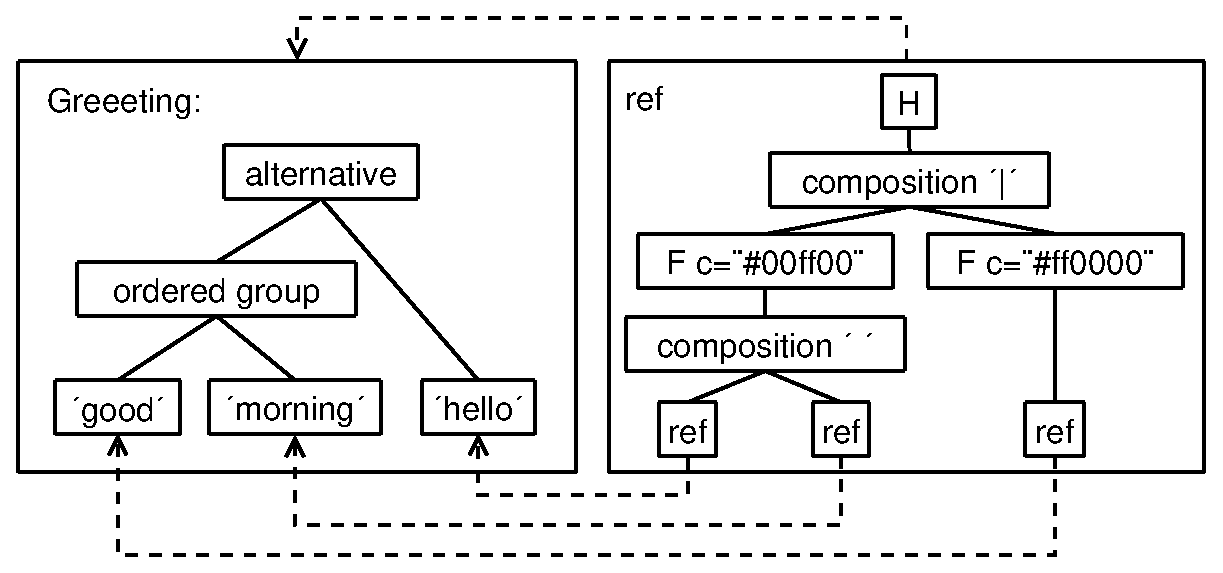
\includegraphics[scale=0.51]{pictures/FormattingRuleStructure.eps}
\label{FormattingRuleStructure}
\end{figure}
\noindent

Usages of the operator that surrounds references or compositions have been typified but it should be possible to be usages of operators surrounded by themselves. This will require some changes in the syntax of a usage of the ideal meta-model because operator's name and a rule call is represented by an identifier it would not be clear which object should be created since \textsc{Xtext}'s parser works with a view to only one token. The solution could be to try to extend parser's outlook but it can be a bit slower than the default variant. A more elegant solution could be enclose the usage of a operator by some keywords. Since angle brackets have not been used so they look like a good choice. 

This problem with usages of operators has been solved. Now it has to be decided which kinds of operators should be allowed to use for these formatting rules. Definitely, it should be enabled positional operators because they give to grammar rule an shape. Further, it should be enabled highlight operators because the \textsc{Xtext} framework contains a concept of semantic highlighting at the semantic level (see the \textit{Section \ref{SyntaxHighlighting}}) and these formatting rules is a good place for an integration of the concept into the configuration of the pretty printer. Since the transforming operators were designed in order to format comments and comments do not exist at this level, they will be disabled.

\begin{expl}\label{GrammarRuleAndFormattingRule}
This example of a grammar rule and its corresponding formatting rule are related to the \textit{Figure \ref{FormattingRuleStructure}}. The same operators are used. The formatting rule is identified by the PBOX keyword because grammar rule for nonterminals are also called parser rules (see the \textit{Section \ref{parserRules}}). 
\begingroup
\fontsize{10pt}{12pt}
\begin{Verbatim}[commandchars=\\\{\}]
// Grammar rule
Greetings:
    'good' 'morning' | 'hello'
;

// Formatting rule
PBOX[Greetings]:
    <H>[<F c="\#00ff00">['good' 'morning'] | <F c="\#ff0000">['hello']]
;
\end{Verbatim}
\endgroup
\end{expl}

\subsubsection{Formatting rules for Terminals}

The situation with defining formatting rules is more easier in comparison with formatting rules for nonterminals. The grammar rule of a terminal does not contain any defining elements like in a grammar rule of a nonterminal. Thus the formatting rule should contain only usages of operators. It also follows that positional operators can not be used in any way. Conversely, transforming operators could be used for formatting comments and highlight operators would serve to define a configuration of syntax highlighting at the lexical level. Furthermore, it makes sense to use maximally one transforming operator and one highlight operator.

Although, terminals defined by terminal rules (see the \textit{Section \ref{TerminalRules}}) exist in the \textsc{Xtext} framework, which can be referenced similarly like nonterminals, the keywords used as a defining element has a terminal character and it would be beneficial to resolve them by various fonts. Since they have no own formatting rule, they should be referenced alternatively. The possible solution is to categorize keywords by regular expression that work on the wanted lexical level. The similar situation is how to define a default font for terminals which do not have any corresponding formatting rule defining a font. The whole solution is typified in the following listing.

\begin{expl}\label{TerminalFormattingRules}
This listing describes possibilities how to define formatting rules for terminals. The first one formats multi line comments. The second one makes all keywords beginning with a letter bold and blue. And the last one makes all other terminals gray.
\begingroup
\fontsize{10pt}{12pt}
\begin{Verbatim}[commandchars=\\\{\}]
// Formatting rule referencing a terminal defined by grammar rule.
TBOX[ML_COMMENT]: <MC>, <F c="#00ff00">;

// Formatting rule with a regular expression 
TBOX[Keyword, "^\textbackslash\textbackslash{}w.*\$"]: <F c="#0000aa", w=bold>;

// Formatting rule for terminals that have no
// formatting rule of two previous categories.
TBOX[default]: <F c="#222222">;

\end{Verbatim}
\endgroup
\end{expl}

\section{Realization}
\label{BoxModelRealization}
All realization steps seem to be straightforward with one exception. The \textit{Section \ref{ScopingOperators}} discusses that it has to be defined some mechanism allowing for creating suitable scopes that are important for referencing parameters of some operator, there are exist a problem how to reference essential defining elements so that it would be possible to reference elements that are on a equivalent position in the tree structure like an identifier of a corresponding cross reference. This problem can not be solved like referencing parameters of operators because connection between a cross reference and its referenced object is created on the base of existence of cross reference's identifier in a scope which is a set of descriptions of possible objects. The object description contain information about its identifier. It means that the scoping in this form does not guarantee any restriction regard to order of elements. Moreover, because composite defining elements are defined by a language developer and hence are defined dynamically, the scopes have to contain identifiers of all defining elements of grammar rule. Thus  it can not be captured any restriction regard to nesting in the tree structure.

One possible solution is to change a method  identifying cross references and corresponding defining elements internally for scoping so that an identifier be able to capture the exact position of a cross reference or defining element in the tree structure. The newly created identifier for the essential defining element and its reference should contain elements name, a number expressing its order in a parent element and parent's identifier where the parent could be an composite element, a grammar rule or a formatting rule. The identifier of a composite element consists of its delimiter, position and parent's identifier. Moreover, grammar rules and formatting rules will be identified by its names, which will allowing for identifying references and defining elements uniquely. Thus the scopes of defining elements  do not have to be define within a grammar rule.

\begin{expl}\label{IdentifiersFormattingElements}
Newly proposed identifiers for the essential defining elements from the \textit{Listing \ref{GrammarRuleAndFormattingRule}}.
\begingroup
\fontsize{10pt}{12pt}
\begin{Verbatim}[commandchars=\\\{\}]
Greetings.|.0. .0.good
Greetings.|.0. .1.morning
Greetings.|.1.hello 
\end{Verbatim}
\endgroup
\end{expl}

The system of creating identifiers is designed and it remains to solve how to implement this change into the code of the \textsc{Xtext} framework.

\subsection{Linking}

The linking cross references to referenced objects is realized in the \textsc{Xtext} framework by a class implementing the \texttt{ILinkingService} interface specially its method \texttt{getLinkedObjects}. The method has tree parameters. The first one called context represents a model element containing a given cross reference. The second one called reference represents a description of a given cross reference. And the last one called node is an element of a \textit{node model} which is an AST-based structure. The node represents a position of a given cross reference in this structure.  The default implementation of the interface gets a required type of from the reference description and it passes the type together with the context to some default scope provider thereby giving a scope. Further, it get an identifier of a given reference from the node which it then uses for getting an object description from the scope. The object description then allows for getting a given object that the method returns.

This behavior of the method is inappropriate with use of  newly designed version of identifiers.  In this case, the user has to enter these long identifiers manually. It follows that it has to be written a new implementation of the interface where the method would contain translating simple identifiers into a new version. Furthermore, it has to be solved how to get the new version of identifiers into object descriptions located in a scope.

\subsection{Identifying Elements Defining a Formatting Rule}

Identifiers are represented in the \textsc{Xtext} framework by the \texttt{QualifiedName} class, which is essentially a name formed from several hierarchical segments. These identifiers can be obtained from the \texttt{getFullyQualifiedName} method, whose only parameter represents object for who is an identifier wanted. This method is specified in the \texttt{IQualifiedNameProvider} interface. Therefore the task how to transform simple identifiers into a new version can be solved by inserting the \texttt{Reference} grammar rule containing only cross reference to a type of essential defining elements into a grammar of this language. Because of this step the instances of the \texttt{Reference} will be located at the same place in the tree structure like essential defining elements. The next step is to write a new implementation of the \texttt{IQualifiedNameProvider} interface  that would involve  the new version of identifiers for the model generated from a code written in this language where each instance of the \texttt{Reference} would have a blank name. Moreover, the implementation has to be registered by utilizing \textsc{Google Guice} in order to be the implementation active. The name from this new implementation would be concatenated with a simple identifier obtained from a node in order to get a whole identifier of the new version.

\subsection{Identifying Elements Defining a Parser Rule}

As the previous problem was solved by creating the new implementation of the \text{IQualifiedNameProvider} interface, a change of identifiers contained in descriptions of defining elements forming scopes into the new version can be realized similarly. Moreover, there is no need to concatenate an identifier from more parts because essential defining elements has name or other attributes that can serve as a simple identifier.  Now it has to be decided how to integrate identifiers of the new version into descriptions The mere registration of the new implementation of the interface by utilizing \textsc{Google Guice} in order to change a default  implementation, which is used by a code creating concrete descriptions, is not sufficient because each language has own \textsc{Google Guice} configuration and the default implementation is registered into configuration of the language defining \textsc{Xtext}'s grammar.

Thus it has to be rewritten a code that is registered under the configuration of this language and serves to obtaining descriptions from another languages. The descriptions are obtained together as a pack represented by the \texttt{IResourceDescription} interface. The place for obtaining descriptions is  located in the \texttt{getResourceDescription} method of the \texttt{LoadOnDemandResourceDescriptions} class, where the method finds out a manager of resource descriptions for a particular language on the base of a URI of resource descriptions forwarded as an only parameter. Further, a selected manager returns a needed resource description. Thus it has to be the method rewritten so as the methods selects newly created manager for descriptions of the language of \textsc{Xtext}'s grammar. The creation of a new manager involves not only to implement \texttt{IResourceDescription.Manager} interface representing a manager but also implement the \texttt{IDefaultResourceDescriptionStrategy} interface that is responsible for creating descriptions and it is exploited by manager. Thus the strategy is the right place for getting a new version of identifiers into object descriptions.

\chapter {Language for Defining Heuristics of the Initial Box Model}
\label{LanguageOfHeuristics}
The \textit{Chapter \ref{GoalsRevisited}} discusses that an imperative or declarative specification of a formatting configuration of a generic pretty printer is time-consuming. Thus this language is able to define some heuristic rules serving to determine how an initial box model for a particular language described by \textsc{Xtext}'s grammar look like. In other words, this language introduces new formatting rules that are independent on a grammar and serve to as an input for a transformation into formatting rules of the \textsc{ModelLang} language. This language is called as the \textsc{HeurLang} in the remaining text. 

\section{Design}

The following text describes what could look like a language defining formatting rules that are independent on a grammar of a language. Firstly, it should be selected an extension for files containing a code of this language. The extension should express the essence of this language like the extensions for two previous languages. This language essentially allows for defining Pretty-Printer's Default formatting configuration, so the extension \textbf{.ppd} will be a good choice. Further, because  this language will be able to define some formatting rules, it will have to use the operators defined by utilizing the \textsc{MetaModLang} language. Since it would be beneficial to use constants defined by that language and the grammar of that language contains grammar rules allowing for defining usages of these constants, the grammar of this language should be inherited from the grammar of the \textsc{MetaModLang} language. Moreover, it would be good to reference a file containing a box meta-model via URI imports in order to be consistent. The heuristic rules will be transformed into formatting rules referencing terminal rules defining terminals and parser rules defining nonterminals so the heuristic rules should be separated into a group dedicated for terminals and a group dedicated for nonterminals in order to make a specification more comprehensible.

\subsection{Heuristic Rules for Nonterminals}

Although, this language will  be able to use operators of a referenced box meta-model, any defining elements of any grammar rule will not be available. Now has to be decided how to specify places inside definitions of grammar rules that that should be enclosed by an usage of an operator. The one solution could be to define an usage of an operator and specify where this usage will be applied. The specification of locations  can be realized only by some pattern determining whether the usage can be placed at a given locations or not similarly like regular expressions determine whether a piece of text is suitable or not.

Now it is necessary to design what these patterns should look like and how should work its evaluation. Firstly, it is good to realize that pieces forming these patterns has to reflect defining elements and also a code described by a grammar rule in order to the patterns be comprehensible. The keyword is only defining element occurring in a specification of a grammar rule whilst also in a code parsed by the grammar rule. Thus the patterns will contain keywords. Rule calls, cross references and composite defining elements do not directly reflects a code parsed by the grammar rule, so they will be represented in patterns by numbers and intervals expressing the multiplicity of their occurrence in the node of a tree structure defining a grammar rule. 

\begin{expl}\label{HeuristicNonterms}
A possible section of  rules for nonterminals in a file defining a heuristic for generating an initial box model. The first rule has a special significance because its usage of an operator serving to enclose the root of a formatting rule. If the question mark is present, the usage could be rewritten by another one which is defined by another rule. The second rule encloses a node of the tree structure by its usage of operator when the first and the last child of the node are parenthesis. The third rule encloses a node  by its usages of operators if the node has tree children and the second is an equal character. The last rule encloses a node by its usage of a operator if the node has at least two children and the last is a colon.
\begingroup
\fontsize{10pt}{12pt}
\begin{Verbatim}[commandchars=\\\{\}]
Non-terminals:
    root? : <V>
    ['(',*,')']: <H>
    [1,'=',1]: <I>,<H>
    [1-*,':']: <H>
\end{Verbatim}
\endgroup
\end{expl}

Some proposal has been typified what the section of heuristic rules dedicated for non-terminals should look like. Now it should be designed how this section be transformed into language-depended formatting rules. The most feasible solution is to transform a model generated from grammar rules of a given language into a box model representing formatting rules without usages of operators firstly. A part of the box model without usages of operators related to nonterminals  has a similar structure like an equivalent part of the grammar model, so patterns of heuristic rules expresses the same thing in a box model as well as in a grammar model. Thus it can be searched places inside a box model that subsequently serve for injecting usages of operators into the box model. 

The searching places and injecting usages of operator could work simultaneously by utilizing the DFS algorithm \cite{DFS} with some following modifications. The traversal of tree structure of a formatting rule begins at the root. If the node is an ordered group, the first heuristic rule is taken and it is tested whether some sub-sequence of node's children satisfies its pattern.  If such a sequence exists, it is subsequently enclosed by usages of parameters defined in the heuristic rule. It causes a division of ordered group into tree pieces. The first one is formed by a sequence of children that are in front of matched sequence. The second is the matched sequence. And the last represents  a sequence of children following after the matched sequence. Now the current node has this tree children. These new tree ordered groups can be reflected into the identifiers of its in order to not change a path which identifiers express. Further, the traversal continues with these new nodes, where the usages of operators are skipped at the second node and the traversal must be careful to not use the same rule on the whole second node. If the matched sequence does not exists, this process is repeated with the next heuristic rule. Further, if there is no heuristic rule left, the traversal  continues with node's children with all heuristic rules. if the node is another type of composite element, it can be matched sequences with only one child because the order of its children does not reflect a parsed code. When the node is a leaf or the algorithm has already visit all node's children, the matching can not take place and the algorithm backtracks.

\begin{expl}\label{GeneratedFromattingRule}
The listing describes two grammar rules of a language allowing for defining some objects and its attributes. The object references some box in which is contained. There are also formatting rules generated from these grammar rules by utilizing heuristic rules defined in the \textit{Listing \ref{HeuristicNonterms}}.
\begingroup
\fontsize{10pt}{12pt}
\begin{Verbatim}[commandchars=\\\{\}]
// Grammar rules
Object:
    'obj' name=ID '(' box=[Box] ')' ':'
	attributes+=Attribute*
   ';'
;

Attribute:
    name=ID '=' value=Value
;

// Generated formatting rules
PBOX[Object]:
    <V>[
        <H>['obj' name:ID <H>['(' box:[Box] ')'] ':']
        attributes:Attribute
        ';'
    ]
;

PBOX[Attribute]:
    <I>[<H>[name:ID '=' value:Value]]
;
\end{Verbatim}
\endgroup
\end{expl}

\subsection{Heuristic Rules for Terminals}

However, nonterminal heuristic rules have to be independent on grammar rules because parser rules are unknown until an user defines them, a situation with terminals is inverse. In most cases a language developer uses default terminal rules so heuristic rules should defines default usages of operators for these terminals. Of course, a developer can add new terminals or use only terminals with only different names but there is the default formatting rule in each definition of formatting rules. The transformation from heuristic rules into formatting rules must only test whether a terminal defined in a heuristic rule exists in a grammar. If the terminal does not exist, the formatting rule is not generated.

\begin{expl}\label{HeuristicNonterms}
A possible section of rules for terminals in a file defining a heuristic for generating an initial box model. The first three heuristic rules define usages of operators for formatting rules that will reference terminals defined before colons. The fourth rule defines an usage of an operator for a formatting rule of the keyword whose regular expression is enclosed in square brackets. The last rule defines an usage of an operator for a default formatting rule.
\begingroup
\fontsize{10pt}{12pt}
\begin{Verbatim}[commandchars=\\\{\}]
Terminals: 
    INT: <F w=bold>
    ML_COMMENT: <F i=italic, c="#00FF00">, <MC>
    SL_COMMENT: <F i=italic, c="#00FF00">, <SC>
    Keyword["^\textbackslash\textbackslash{}w.*\$"]: <F c="#FF0000">
    default: <F>
\end{Verbatim}
\endgroup
\end{expl}

\section{Realization}
\label{HeurRealization}
The steps to implement the language designed in the previous section are straight-forward or similar to realization steps described in the previous two chapters but there are some questions concerning what implementation resources should be used for the realization.

\subsection{Model Traversal}

When it is needed to transform a model into an another model, the model has to be somehow traversed. The traversal is formed from many steps where the step represents to perform certain actions and choose a next element of model. It requires to know a type of a currently visited element and find actions competent for the type.  The action searching can be realized in \textsc{Java} only by if statements or a switch statement deciding by element's type thus requiring to write a lot of code. The facilitation could be to write the model traversal in the \textsc{Xtend2} language \cite{Xtend}.  This language contains a concept called dispatch methods. These methods behave polymorphically based on types of method's parameters. In other words, When the method has more overloads and it is called with a parameter that have got a specific type and it is somehow retyped, it is chosen a variant of the method with a specific type. Moreover, the types of parameters of method's overloads do not have to be in the inheritance hierarchy. The \textsc{Xtend2} language can easily call a \textsc{Java} code because a code written in  \textsc{Xtend2} is transformed into \textsc{Java}.

\begin{expl}\label{HeuristicNonterms}
A comparison of behavior of overloaded \textsc{Java} methods  and  dispatch methods of the \textsc{Xtend2}  language.
\begingroup
\fontsize{10pt}{12pt}
\begin{Verbatim}[commandchars=\\\{\}]
class A \{\}
class B extends A \{\}

// Java code
class Main
\{
    public static void main(String[] args)
    \{
        Main main = new Main();
        B obj = new B();
        main.foo((A)obj);
    \}
	
    void foo(A par)
    \{
        System.out.println("A");
    \}
	
    void foo(B par)
    \{
        System.out.println("B");
    \}
\}

// Result: A

// Xtend 2 code
class Main
\{
    def static void main(String[] args)
    \{
        Main main = new Main();
        B obj = new B();
        main.foo((A)obj);
    \}
	
    def dispatch void foo(A par)
    \{
        System.out.println("A");
    \}
	
    def dispatch void foo(B par)
    \{
        System.out.println("B");
    \}
\}

// Result: B
\end{Verbatim}
\endgroup
\end{expl}

\subsection{Model Transformation into a Text Representation}
\label{XpandModelTransformation}
A tool for traversing models and translate them into another models were introduced. It can be obtained an initial box model from heuristic and grammar rules by this way. Because of a language developer be allowed to change the box model, it has to be transformed into a corresponding domain-specific language. Standardly, the~\textsc{XPand}~languages~\cite{XPand} and the \textsc{Acceleo}~language~\cite{Acceleo} serve for this purpose. The languages allow for defining templates representing the mapping of a certain model into a certain language. An another option is to use the \textsc{Xtend2}~language~\cite{Xtend} that contains a similar concept of templates. Moreover, the language is able to work as a classical imperative and object-oriented language. Since the \textsc{Xtend2} language is used for traversing models and these two parts of realization are related between themselves, it should be the \textsc{Xtend2} used again.

\begin{expl}\label{HeuristicNonterms}
An listing of a method that works as a template. The method transforms imports of a box model into their text declarations. The templates are indicated in the \textsc{Xtend2} language by the sequence of three apostrophes and the template can reference an outside variables by a code enclosed in "«"  and "»".
\begingroup
\fontsize{10pt}{12pt}
\begin{Verbatim}[commandchars=\\\{\}]
def placeImports(BoxModel boxModel)'''
     «FOR imp:boxModel.operatorsSection.imports»
         import "«imp.importURI»"
     «ENDFOR»
'''

\end{Verbatim}
\endgroup
\end{expl}

\chapter {Integrating the Box Model into the Xtext framework}
So far resources allowing for defining box models were introduced but it has not been mentioned how to interconnect box models with pretty-printing concepts contained in the \textsc{Xtext} framework (see the \textit{Section~\ref{CodeFormatting}} and the \textit{Section~\ref{SyntaxHighlighting}}) yet. The purpose of this chapter is to design a solution of this problem. In other words, it has to be designed behavioral implementations of operators so that be able to cooperate with a code of the \textsc{Xtext} framework realizing code formatting (see the \textit{Section~\ref{CodeFormatting}}) and syntax highlighting (see the \textit{Section~\ref{SyntaxHighlighting}}). 

\section{Syntax Highlighting}

 The \textit{Section~\ref{SyntaxHighlighting}} discusses that this concept is essentially an associating defined text styles with individual parts of code. Moreover, the process of association can be realized lexically or semantically. These two ways correspond to usages of highlight operators in terminal formatting rules (the lexical way) and parser formatting rules (the semantic way).

\subsection{Behavioral Implementation of Operators}
 The definition of a highlight operator written in the corresponding DSL is formed from parameters whose current values together specify a particular text style (see the \textit{Section~\ref{BasicOperators}}) and text styles are realized in the \textsc{Xtext} framework by the \texttt{TextStyle} class (see the \textit{Listing~\ref{HighlightingConfiguration}}). Thus the behavioral implementation of an operator should translate a text style expressed by values of parameters into the \texttt{TextStyle} class. Moreover, it should be only one implementation enough  because highlight operators and its usages differ only in values of parameters.

\subsection{Highlighting Configuration}
\label{HighlightingConfiguration}
Before text styles be able to associated with parts of some code, they have to be registered (see the \textit{Section~\ref{TextStyles}}). The text styles specified by usages of highlight operators can be registered by creating a new implementation of the \texttt{IHighlightingConfiguration} interface (see the \textit{Listing~\ref{HighlightingConfiguration}}) that would have an access to a box model describing a formatting configuration for a given language. The implementation would override the \texttt{configure} method so that the method get all usages of highlight operators from all formatting rules and instantiate a behavior implementation related to each usage. A given behavior implementation translates values of usages into the \texttt{TextStyle} class and the method registers it under a specific identifier. 

The task how to choose a suitable identifier for text styles related to usages from formatting rules dedicated for terminals is simple. If the formatting rule is the default, the identifier will be the string "default". Further, if the formatting rule references a terminal rule, the identifier will be a name of the terminal rule. But also if the formatting rule specifies an appearance of keywords matching to a certain regular expression. Since identifying text styles by regular expressions is confusing, the corresponding formatting rule will be enriched with name, which will serve as an identifier for the text style, such as depicted in the \textit{Listing~\ref{TerminalFormattingRules}}.

The situation of identifying text styles defined by usages contained in formatting rules referencing formatting rules is not so easy because the usage has not unique identifier and this kind of formatting rule can contain more usages of operators. Thus it has to be created a new concept of identifying these text styles. One possible solution is to create identifiers from a name of the parser rule and a suffix expressing hierarchical position of an usage of an operator among other usages contained in the formatting rule. The following listing typifies a format of identifiers for these usages of operators.

\begin{expl}\label{ParserRuleIdentifiers}
The listing shows what identifiers for usages of operators presented in the \textit{Listing~\ref{GrammarRuleAndFormattingRule}} look like.
\begingroup
\fontsize{10pt}{12pt}
\begin{Verbatim}[commandchars=\\\{\}]
<H> : Greetings.1
<F c="\#00ff00"> : Greetings.1.1
<F c="\#ff0000"> : Greetings.1.2
\end{Verbatim}
\endgroup
\end{expl}

\subsection{Lexical Highlighting}

The \textit{Section \ref{LexicalHighlighting}} discusses that associating text styles to parts of code lexically can be realized in the \textsc{Xtext} framework by extending the \texttt{AbstractAntlrTokenToAttributeIdMapper} class and overriding its \texttt{calculateId} method. Since lexical highlighting is a only matter of formatting rules dedicated for terminals, the \texttt{calculateId} method of a new extension having an access to the box model will work as follows. If a value of the \texttt{tokenName} parameter will have the "RULE\_" prefix, the token is parsed  by utilizing a terminal rule, it will be searched a corresponding formatting rule for terminal rule by the token name without the prefix in the box model. If the formatting rule exists and contains an usage of a highlight operator, it will be returned an identifier of a corresponding text style. If a value of the token name is enclosed in apostrophes or quotation marks, the token is a keyword and subsequently will be tried whether the keyword matches to pattern of any keyword formatting rule. If the formatting rule exists and contains an usage of a highlight operator, it will be returned an identifier of a corresponding text style. In case it is not returned any identifier based  on the previous conditions, it will be returned the identifier of the default text style.

\subsection{Semantic Highlighting}

The \textit{Section \ref{SemanticHighlighting}} discusses that associating text styles to parts of code in a semantic way can be realized in the \textsc{Xtext} framework by implementing the \texttt{ISemanticHighlightingCalculator} interface and overriding its \texttt{provideHighlightingFor} method that should contain callings of the \texttt{addPosition} method on the second parameter which it associates some segment of code with some text style. Bounds of individual segments of a code reflecting semantics can be obtained from the first parameter because the parameter allows for getting a node model, which is an AST-based structure, and elements of the node model have informations about bounds of segments. Although, an element of the node model is linked to corresponding defining element of a grammar rules, it has not clear yet how to get a corresponding text style defined by an usage of an operator. Each defining element has a composite element or reference in a formatting rule and also it shares the same qualified name with the element of formatting rule as it is shown in the \textit{Listing \ref{IdentifiersFormattingElements}}. Moreover, it is unknown which text style belongs to the element of formatting rule. 

A solution solving the whole problem could be to create an initialization of a new implementation of the interface. The initialization would involve a traversal of formatting rules referencing parser rules. The traversal will serve to clarify which usage of some highlight operator is a closest ancestor of a certain element of a formatting rule. The result of the traversal will be a map containing associations between qualified names of elements of formatting rules and identifiers of text styles related to usages of highlight operators that are closest ancestors of given elements. Since the qualified name contained  in the map can also belong to a defining element of a grammar rule, the \texttt{provideHighlightingFor} method of the new implementation will exploit the map to obtain an identifier of text style for a given segment of code. It may become the situation that an element of formatting rule has no ancestor that is an usage of a highlight operator and thus its identifier is not in the map. In this case, the method will use the identifier of the default text style. Moreover, the map do not have to contain identifiers of composite defining elements because elements of the node model reference only essential defining elements.

\begin{expl}\label{Map}
The listing depicts what a map for grammar that contains one rule presented should look like in the \textit{Listing \ref{GrammarRuleAndFormattingRule}}. Identifiers of defining elements  are obtained from the \textit{Listing \ref{IdentifiersFormattingElements}} and identifiers of text styles from the \textit{Listing \ref{ParserRuleIdentifiers}}.
\begingroup
\fontsize{10pt}{12pt}
\begin{Verbatim}[commandchars=\\\{\}]
Greetings.|.0. .0.good -> Greetings.1.1 // <F c="\#00ff00">
Greetings.|.0. .1.morning -> Greetings.1.1 // <F c="\#00ff00">
Greetings.|.1.hello -> Greetings.1.2 // <F c="\#ff0000">
\end{Verbatim}
\endgroup
\end{expl}

It might seem that some conflicts exist in associating text styles with a concrete segment of code because a node having some children covers the same code like its children together. But if the method will traverse a node model so that the parent node will be visited firstly and the its children, there will be no conflict because the \textsc{Xtext} framework allows a developer to redefine a text style for an arbitrary segment of code.

\section{Code Formatting}
\label{CodeFormattingRealization}
The \textit{Section \ref{CodeFormatting}} discusses that code formatting can be realized in the \textsc{Xtext} framework by extending the \texttt{AbstractDeclarativeFormatter} class and overriding the \texttt{configureFormatting} method, which has only one parameter. Calling methods on the parameter serves to creating a formatting configurations for a particular grammar. Since rules of this formatter only allows a developer to statically define mutual positions of tokens by utilizing defining elements of grammar rules and have no information about formatted tokens, it can not be expressed behavior of horizontal-vertical operators formatting tokens on the base of the total length of tokens by this way. Thus  specifying code formatting by utilizing a box model can not be realized through the original method of specification as well as specifying syntax highlighting is realized.

After thoroughly reading trough the code of the \textsc{Xtext} framework it is possible to find out that higher layers of \textsc{Xtext}'s code exploits some implementation of the \texttt{INodeModelFormatter} interface to format code. Any implementation of this interface has to contain an overriding of the format method. The method has three parameters where the first one is  a node model of formated code, the other parameters are offset and length of a code dedicated to be formated. Moreover, the method has to return an instance of the \texttt{IFormattedRegion} interface containing a string of already formatted code, an offset and length. The default implementation of this interface uses the \texttt{OneWhitespaceFormatter} class or extension of the \texttt{AbstractDeclarativeFormatter} class to know how code should be formatted. Thus the interconnection between \textsc{Xtext}'s code dealing with code formatting and a box model can be realized by creating a new implementation of the \texttt{INodeModelFormatter} interface that would exploit some box model as well as the default implementation uses mentioned formatters. Further, it would be better if the implementation did not inherit from the interface directly but the implementation was extended from the \texttt{AbstractNodeModelFormatter} class containing the default implementation of the \texttt{IFormattedRegion} interface as an inner class.

\subsubsection{Positional Operators}
Since behavior implementations of positional operators will represent inner nodes of the formatting tree structure, they should contain references to children. Some implementations have to know how a code formated by its children will be length in order to select a variant of behavior. This is the case of behavior implementations of horizontal-vertical operators. But also behavior of a parent in the formatting tree structure can affect behavior of its children such as a indenting operators only if its parent formats vertically. Thus it has to be firstly calculated how the parent should work. Since obtaining information about length from formatted code from children, which may be recalculated several times, is slow, implementations should contain dedicated methods for obtaining  length of the first row, length of the last row, length of the largest row and count of rows of a potential formatted code.


Although, behavior implementations of most of positional operators will assemble formated code of their children as well as some inner node of a node model expresses whole code represented by its children, it can be found some positional operators whose behavior implementation will not assemble formated code of their children but will add some spacing characters to formated code of each child and will leave assembling to its parent. A good example is the indenting operator. Thus behavior implementations of this kind will be cloned so many times that each child will have own behavior implementation of this kind as a parent in order to behavior implementations be consist.


\subsection{Implementing Concept}
The next step is to describe how the format method of the new implementation of the \texttt{INodeModelFormatter} interface should work. The method can utilize the node model of a formatted code and  a box model expressing how the code should be formatted. Since leafs of the node model represent particular tokens and character sequences of an original code formatting and other nodes are related to rule calls, the solution could be to transform the node model into an another tree structure expressing the code formatted by a box model. The new tree structure  should also contain tokens as leafs or if a token corresponds to a terminal rule for which a usage of transforming operator exists, the token would be replaced by the behavior implementation of the transforming operator that encapsulates the token. Other nodes of the tree structure would be represented by behavior implementations of positional operators thus ensuring relative positioning between tokens. 

The transformation of the node model to the new tree structure should be carried so that leafs are transformed at first and other nodes are subsequently transformed from lower to higher layers. Since the inner node of the node model represent a rule call of a parser rule, the inner node will be transformed into a tree structure of the behavior implementations that corresponds to usages of positional operators from a formatting rule dedicated for the given parser rule. In order to this concept make sense, behavior implementations have to be initialized by values of usages of positional operators. Moreover, the formatting rules related to a parser rule have to contain an usage of a positional operator as  root of the definition of the formatting rule and each parser rule of a given grammar has to have one formatting rule in the box model.

\begin{figure}[h!]
\centering
\caption{A schema depicts a partial node model of some code whose some grammar rules are presented in the \textit{Listing \ref{GeneratedFromattingRule}}. There are some gray nodes expressing sequences of blank characters from the original formatting. The node model is transformed into a formatting tree structure of behavior implementations, which is inspired by formatting rules from the same listing.}
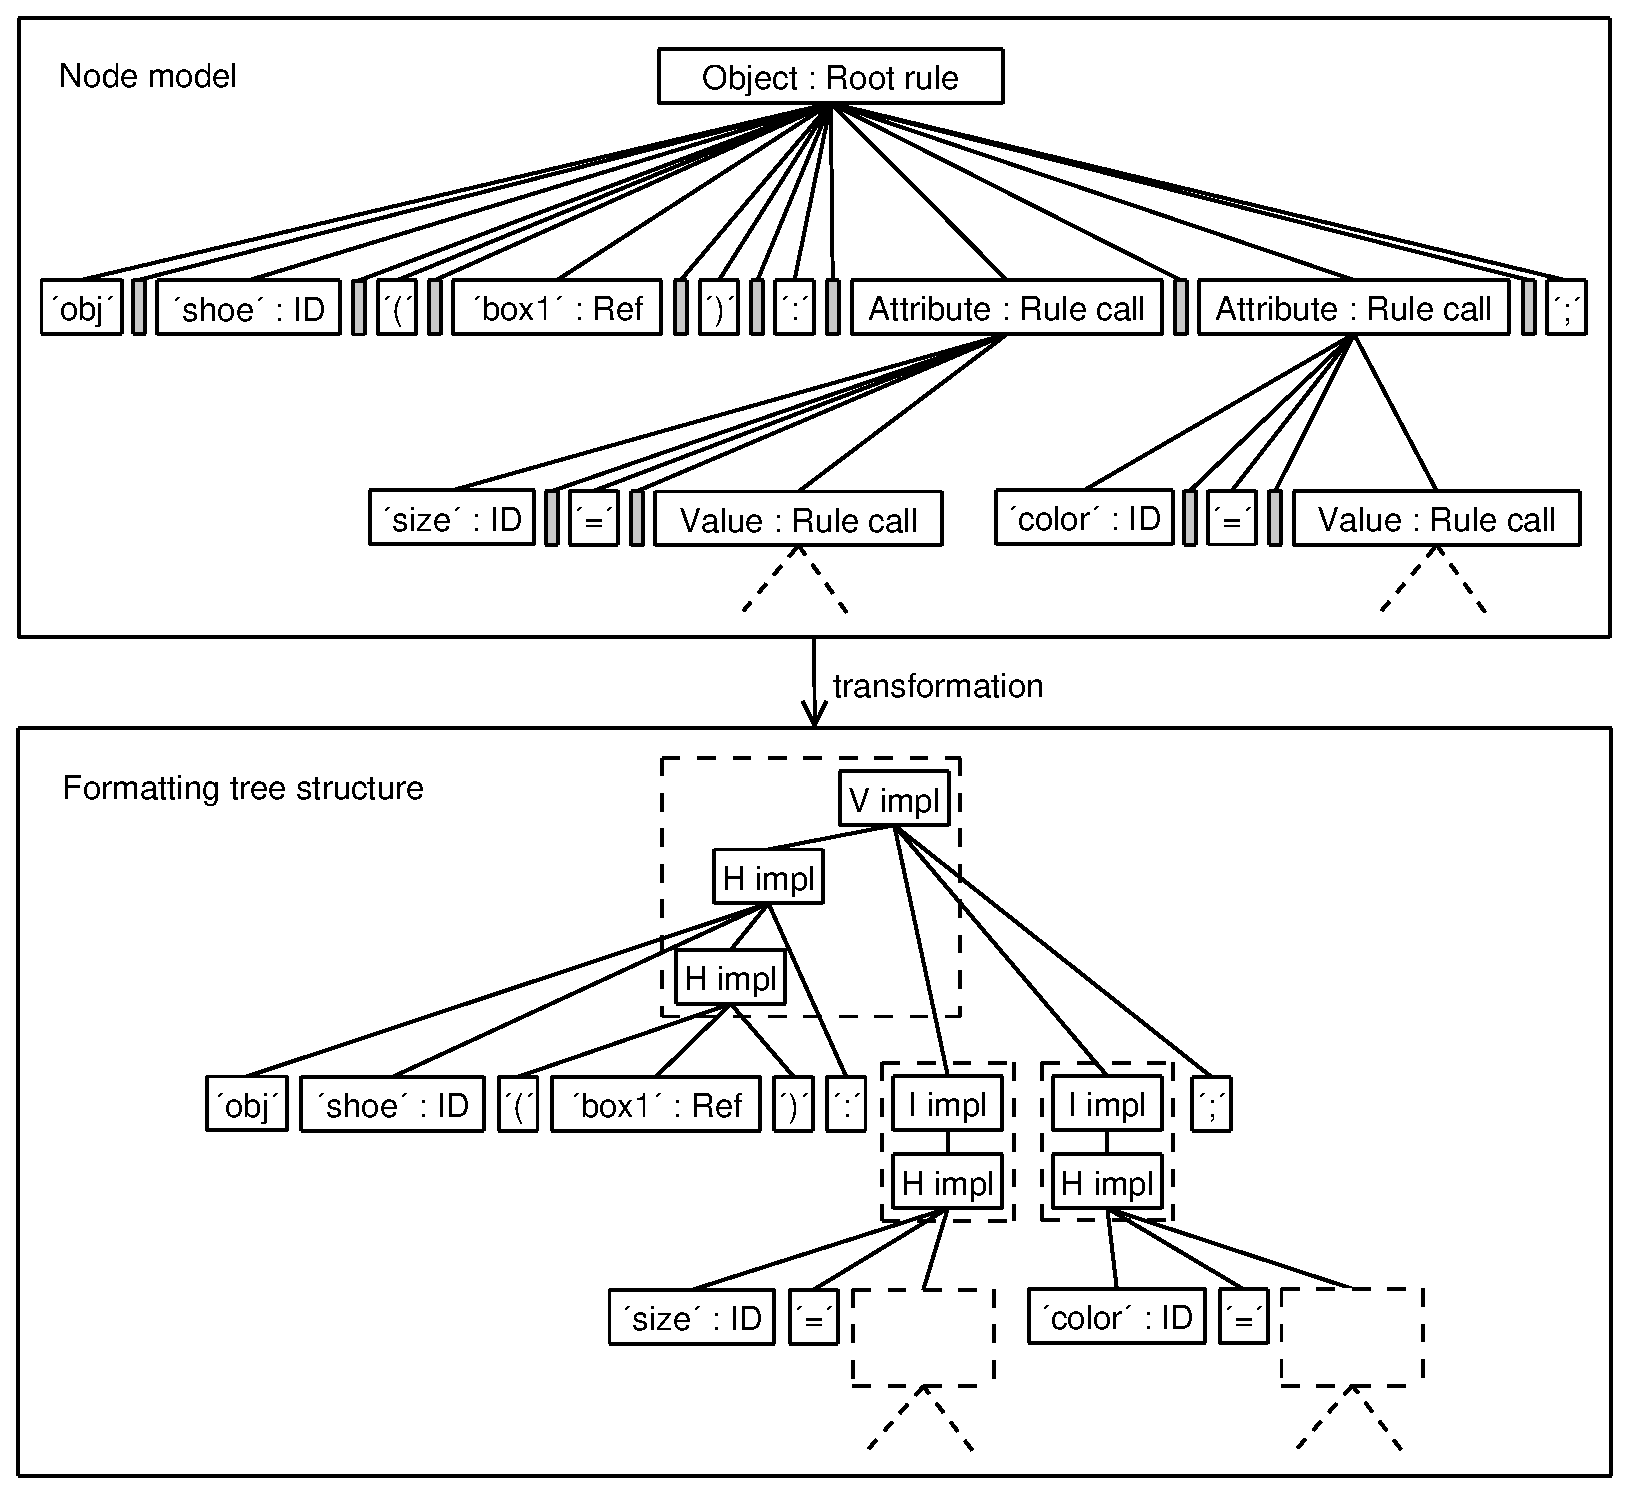
\includegraphics[scale=0.51]{pictures/NodeModelFormatting.eps}
\label{NodeModelFormatting}
\end{figure}
\noindent

The transformation of a node model into formatting tree structure might seem straightforward. But a node model differs from the classical AST in some cases.  These distinctions are a consequence of integrating actions defined in a grammar (see the \textit{Listing~\ref{Action}}) into the node model and they have to be eliminated during the transformation. 

\begin{figure}[h!]
\centering
\caption{A schema depicts a segment of a node model of some code whose some grammar rules are presented in the \textit{Listing \ref{grammar}} and expresses how the node model might differ from a classical AST when the grammar contains some rules with actions.}
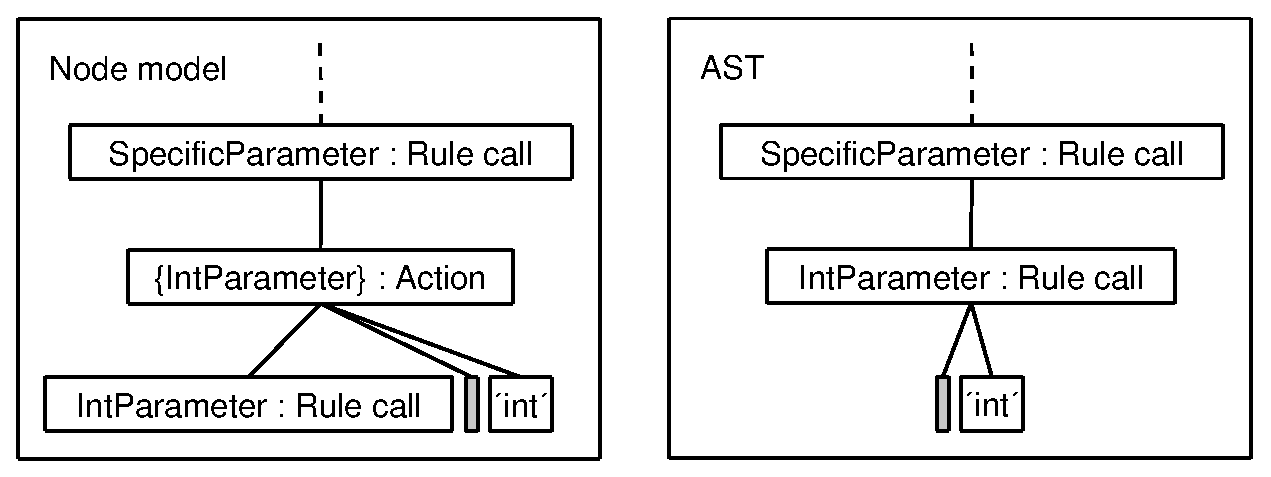
\includegraphics[scale=0.51]{pictures/ActionDistinction.eps}
\label{ActionDistinction}
\end{figure}
\noindent


The next step of the formatting procedure would be to serialize the new tree structure into text so that the implementations will recursively apply its behavior from leafs to  root. 

\subsection{Behavioral Implementation of Operators}

It has already been roughly mentioned what  behavior implementations of transforming and positional operators should look like. Now behavior implementations will be considered in greater detail.

Since behavior implementations of both kinds of operators have to work according to values of usages of operators, behavior implementations should contain a method that initializes a given implementation by values of usages of operators.

\subsubsection{Transforming Operators}

Since behavior implementations of transforming operators will serve as leafs in the formatting tree structure, they should allow for storing original tokens in themselves. But they also should be able to transform these tokens into a required format by a new dedicated method.

\section{Workflow}

Languages allowing a user to manage a generic pretty printer and realization concepts of a generic pretty printer following the original code of the \textsc{Xtext} framework were designed in the previous text. It occurs one problem how to propagate these innovations into the \textsc{Xtext} framework so that a language developer can use the generic pretty printer designed by this way and do not have to register all partial changes of a implementation of syntax highlighting and code formatting for developed language in a \textsc{Google Guice} configuration manually. Moreover, it has to be somehow solved how to activate generation of an initial box model from heuristic rules.

The \textit{Section \ref{MWE}} discusses that the behavior of the \textsc{Xtext} framework can be customized so that a workflow configuration file dedicated for a developed language allows for choosing which and how concepts of the framework (see the \textit{Section~\ref{WorkflowConcepts}}) will be used for the language. The workflow configuration file consists of declarations of used components. These components serves to erase old generated code and other useful task, but the most important component is called \texttt{Generator} serving for generating a meta-model from a grammar, generating code of frameworks concept for developed language and register it into a \textsc{Google Guice} configuration. This component delegates its tasks to some subcomponents called \textit{fragments}. The fragment is an arbitrary class extending the \texttt{AbstractGeneratorFragment} class. A developer of a new fragment can override the method for checking fragment's parameters defined in the workflow configuration file, methods allowing for adding some binding rules into a \textsc{Google Guice} configuration and not least methods that generate code into dedicated directories for framework's concept and have access to a grammar of a developed language.

The previous paragraph indicates that the workflow configuration file seems like a good way how the language developer could set the designed generic pretty printer as a pretty printer for a developed language. Utilization of this concept would require creating a fragment that would add bindings for new implementation of syntax highlighting, a fragment that would add bindings for new implementation of code formatting, a fragment that would obtain a box model from a corresponding DSL file and would mediate it to implementation of pretty printing concepts, but also a fragment allowing for starting generating an initial box model from heuristic rules. Realizations of the first two fragments is straight-forward as resulting from the previous so the following text will discuss only realizations of the last two.

\subsection {Starting Generation of the Initial Box Model}
\label{StartingGeneration}
The main purpose of this fragment would be to generate a DSL file containing an initial box model. Therefore a model of heuristic rules  has be obtained from a corresponding DSL file, transformed to a box model which will be subsequently stored in the textual form. Standardly, the \textsc{Xtext} framework generates an model provider obtaining  models from a DSL file together with generation of a meta-model. Further, because generating methods of fragments have an access to grammar, the transformation can be done according to the design from the \textit{Chapter \ref{LanguageOfHeuristics}}. The \textit{Section \ref{XpandModelTransformation}} discusses that obtaining an initial box model from heuristic rules and its serialization into DSL code should be realized by utilizing the \textsc{Xtend2} language. But the \texttt{Generator} component contains a concept of code generation dedicated for its fragments realized by utilizing templates of the \textsc{Xpand}. This problem can be solved by utilizing extensions of templates written in the \textsc{Xtext1} language \cite{Xtend1} which is completely different from \textsc{Xtend2}. Since extensions allow for calling \textsc{Java} code, it can be used the design from the \textit{Chapter \ref{LanguageOfHeuristics}}. All these facts will allow a user to start up generating an initial box model when \textsc{Xtext}'s workflow will be running.

\subsection {Mediation of a Box Model}

This fragment should mediate a box model for concepts of the generic pretty printer, which will subsequently use it. Obtaining a box model can be realized by utilizing a corresponding provider as it was mentioned in the previous section. Since the \textit{Section \ref{HighlightingConfiguration}} designs usages of operators that will have own qualified names, the box model should be post-processed and given names be calculated in order to qualified names do not have to be calculated from scratch at each request to obtain them. Therefore the one solution how to mediate a box model in a rational form could be that this fragment creates an provider that obtains a model from a DSL file, post-processes it, offers it to concepts of generic pretty printer. Another solution could be that the fragment obtains a box model from a DSL file, post-processes it, stores it into a XMI file \cite{XMI} and creates a provider that loads a box model from the XMI file and offers it to concepts of generic pretty printer. This solution moves the time requirements associated with calculation of qualified names from the run time of pretty printer into the run time of the code generation, where speed is not so important.


\chapter{Evaluation}

This chapter evaluates the proposal presented in previous four chapters. The evaluation is based on behavior of a prototype, in which the proposal is implemented. The prototype is available as an appendix of this thesis.  

\section{Comparison of the Designed Generic Pretty Printer against the Original Pretty Printer}\label{SolutionComparision}
The proposal may has advantages but also disadvantages against the original solution of pretty-printing concept in the \textsc{Xtext} framework. The tested basis in the form of a grammar should be not to extensive in order to be clear and understandable but it also should capture most of options of a grammar. The grammar was introduced that serves to the descriptive demonstration of options  of \textsc{Xtext}'s grammar in the \textit{Listing \ref{grammar}}. Thus this grammar looks like as a good choice. Moreover, it has already exist the formatting configuration of the original solution in the \textit{Listing \ref{abstractDeclarativeFormatterExample}} dealing with code formatting  and the \textit{Listing \ref{HighlightingConfigurationExample}}, the \textit{Listing \ref{LexicalHighlightingExample}}, the \textit{Listing \ref{SemanticHighlightingExample}} dealing with syntax highlighting. The pretty-printing effect of the mentioned instance of the original solution can be seen in the \textit{Listing \ref{formattedCode}}. Now it just remains to create an alternative instance of the new solution having the same pretty-printing effect. Such an instance is presented in the following listing.

\begin{expl}\label{ParserRuleIdentifiers}
A box model related to grammar from the \textit{Listing \ref{grammar}}, whose pretty-printing effect is reflected in the \textit{Listing \ref{formattedCode}}. 
\begingroup
\fontsize{10pt}{12pt}
\begin{Verbatim}[commandchars=\\\{\}]
xtext "platform:/resource/cz.gpp/src/cz/gpp/Example.xtext"

import "platform:/resource/gpp/settings/operators.ppo"

TBOX[Default]: <F>;
TBOX[INT]: <F c="#7F7F7F">;
TBOX[ML_COMMENT]: <F i=italic,c="#00FF00">, <MC>;
TBOX[SL_COMMENT]: <F i=italic,c="#00FF00">, <SC>;
TBOX[Keyword, ["^\textbackslash\textbackslash{}w.*\$"]: <F w=bold,c="#7F0055">;

PBOX[Model]:
    <V vs=2>[
        package:Package
        (<V>[imports:Import] & class:Class)
    ]
;
PBOX[QualifiedName]: <H hs=0>[ID ('.' ID)];
PBOX[Package]: <H>['package' name:QualifiedName];
PBOX[Import]: <H>['import' className:QualifiedName];
PBOX[Class]:
    <V>[
        <H>[
            abstract:'abstract' 'class' name:ID
            ('extends' superClass:[Class|ID])
        ]
        '\{'
        <I>[<V vs=2>[(methods:Method | internalClasses:Class)]]
        '\}'
    ]
;
PBOX[Method]:
    <V>[
        <H>[
            visibility:Modifier returnValue:[Class|ID]
            <H hs=0>[
                <F i=italic,c="#55007F">[name:ID] '('
                (parameters:Parameter <H>[(',' parameters:Parameter)])
                ')' '\{'
            ]
        ]
        <I>[<H>[body:INT]]
        '\}'
    ]
;
PBOX[Parameter]: <H>[SpecificParameter name:ID];
PBOX[SpecificParameter]:
    <V>[IntParameter | StringParameter | ObjectParameter]
;
PBOX[ObjectParameter]: <V>[type:[Class|ID]];
PBOX[IntParameter]: <V>['int'];
PBOX[StringParameter]: <V>['string'];
\end{Verbatim}
\endgroup
\end{expl}

\subsection{Discussion}

Both solutions pretty-print the code from the \textit{Listing \ref{formattedCode}} with the same result. The comparison of both formatting configurations gives following facts.
\begin{itemize}
\item \textbf{F1} - Entire code without comments of the formatting configuration of the original solution takes 6250 bytes of space whilst the box model of the new solution in the textual form takes 1267 bytes. Thus the new solution brings not only space saving but also saving of time required for defining some formatting configuration. 
\item \textbf{F2} - Although, somebody can admit that space saving do not have to imply time saving because writing a formatting configuration of the original solution is supported by code completion and the content assist for \textsc{Java} in the \textsc{Eclipse IDE}, the prototype of the new solution offers equivalent features for the \textsc{ModelLang} language.
\item \textbf{F3} - The next possibility how to reduce code of formatting configuration is to use some initial code and modify it. The original solution allows for generating only a skeleton class that extends the \texttt{AbstractDeclarativeFormatter} class, with tree lines of formatting rules, which are mostly replaced by whole core of formatting rule. Thus the only code which will be contained in the result formatting configuration is a prototype of a class that extends the \texttt{AbstractDeclarativeFormatter} class and a prototype of the \texttt{configureFormatting} method, which it represents 172 bytes of space when the class named \texttt{ExampleFormatter}. The opposite situation occurs with the new solution.  A language developer can generate an initial box model by utilizing some prepared heuristic rules capturing similarities of languages that the developer met and subsequently modify the model into a required form. Otherwise, the developer can create some heuristic rules dedicated for a given language and generate an initial box model. This kind of heuristic rules dedicated for the grammar form the \textit{Listing \ref{grammar}} is located in the following listing and takes 425 bytes of space. Subsequently generated textual form of a initial box model takes 1311 bytes and the final box model, which has the same pretty-printing effect like the box model created from scratch, takes 1392 bytes, where the box model was created by adding except few modifications. The difference in the size of this box model and the box model created from scratch is formed by code formatting and some extra usages of operators that has been generated into the initial box model and have no effect in theirs context such as an usage of the horizontal operator that is encapsulated by an another usage of the horizontal operator. The prototype of the new solution also offers the content assist for the \textsc{HeurLang} language. Thus a creation of heuristic rules would be faster.
\begin{expl}\label{HeuristicRulesForEvaluation}
Some heuristic rules dedicated for generating an initial box model for the grammar from the \textit{Listing \ref{grammar}}.
\begingroup
\fontsize{10pt}{12pt}
\begin{Verbatim}[commandchars=\\\{\}]
operators "platform:/resource/gpp/settings/operators.ppo"

Terminals: 
    INT: <F c="#7F7F7F">
    ML_COMMENT: <F i=italic, c="#00FF00">,<MC>
    SL_COMMENT: <F i=italic, c="#00FF00">,<SC>
    Keyword["^\textbackslash\textbackslash{}w.*\$"]: <F w=bold,c="#7F0055">
    default: <F>

Non-terminals:
    root? : <V>
    ['package'|'import',1-*] : <H>
    [1-*,')','\{'] : <H>
    ['\{',*,'\}'] : <V>
    [*,'class',*] : <H>
    [',',1] : <H>
\end{Verbatim}
\endgroup
\end{expl}

\item \textbf{F4} - However, a formatting configuration of the original solution fulfills its purpose, the formatting configuration is confusing because a language developer has no direct reference to the grammar and he has to hold a structure of the grammar in his mind. Moreover, this solution deals with internals of the \textsc{Xtext} language, which a language developer has to more or less know. The new solution is the exact opposite from this perspective.
\item \textbf{F5} - When an user wants to use some software, he often requires software's reliability. The original solution has been developed for many years and it has been tested on many projects. Thus it can be expected that this solution is quite reliable. On the contrary, the new solution is realized by the prototype that has been tested on few projects and therefore it may contain some potential malfunctions.
\item \textbf{F6} - However, both solutions are able to format code matching a given grammar, the situation around formatting code containing some errors is not unambiguous. Since it suffices the original solution that a type of token occurs in the input stream and an formatting sequence together with the token is inserted into the output stream without respect to correctness of previous and following tokens, the original solution is  at least a bit able to format incorrect code. Whereas incorrectness of code may break the construction of operator tree because given elements of the node model do not have corresponding grammar rules that are supposed by a box model (see the Section \ref{CodeFormattingRealization}).

\end{itemize}

\subsection{Summary}
The comparison of the original solution and the new solution were discussed in the previous section. Now the advantages and disadvantages derived from the comparison are formed into an organized table, which is located in the following figure. 

\begin{figure}[h!]
\centering
\caption{A table concludes evaluation of the original and the new solution. When a solution receives more stars in a given aspect, the solution is better.}
	\begin{tabular}{| l | c | c |}
		\hline
		 &
			\textbf{The original solution} &
			\textbf{The new solution}
			\\
		\hline
		\textbf{F1} - Amount of Code & $\bigstar$ & $\bigstar\bigstar\bigstar$ \\
	           \textbf{F2} - Content Assist & $\bigstar\bigstar\bigstar$ & $\bigstar\bigstar\bigstar$ \\
		\textbf{F3} - Initial Configuration & $\bigstar$ & $\bigstar\bigstar\bigstar$ \\
		\textbf{F4} - Comprehensibility &   & $\bigstar\bigstar\bigstar$ \\
		\textbf{F5} - Potential Reliability & $\bigstar\bigstar\bigstar$ & $\bigstar\bigstar$ \\
		\textbf{F6} - Incorrect Code & $\bigstar\bigstar$ &  \\
		\hline
	\end{tabular} \\
\label{ComparisionTable}
\end{figure}
As it can be seen in the previous figure the new solution has most of advantages against the original solution. Moreover, the one from two disadvantages can be removed by longer-term testing and development.



\section {The Generic Pretty Printer Formatting  Code from the Real World}
As it results from the previous section that the prototype of the new solution can pretty-print the code from the \textit{Listing \ref{formattedCode}} that matches the grammar having rather illustrative character. Thus  the prototype was being tested the grammar of the \textsc{MetaModLang} language and it pretty-printed definitions of operators.  Further, three projects were selected, which contain grammars with reasonable size and corresponding  code examples, in a database \cite{XtextCommunity} of grammars written by utilizing the \textsc{Xtext} framework, specifically the \textsc{Protobuf4e} project \cite{Protobuf}, the \textsc{Xtext-typesystem} project \cite{Xtexttypesystem} and the \textsc{XTypeS} project \cite{XTypeS}. In order to the projects be well arranged and deprive of theirs malfunction, they were trimmed of code unrelated to grammar. Moreover, the \textsc{Protobuf4e} project had to be transformed into a new project utilizing the second version of the \textsc{Xtext} framework, because the original project exploits the first version and the modeling workflow engine (see the \textit{Section \ref{MWE}}) is incompatible beetween the versions of the \textsc{Xtext} framework. Further, the grammars contained the projects had to be a little changed. Names of assignments (see the \textit{Section \ref{grammarElements}}) were not allowed to be the same like keywords contained in the \textsc{MetaModLang} and the \textsc{ModelLang} language, because these names were parsed as keywords by lexical analysis of the parser in a file of a box model. Nothing else had to be changed and box models were written for the grammars that allowed for pretty-printing code examples.

\section{Unimplemented Operators}
\label{UnimplementedOperators}
The goal \textbf{G2} was introduced in order to realize operators of the ideal box meta-model in the \textit{Chapter 4}. All operators except the \textbf{ALT} and the \textbf{WD} operator has been successfully implemented. The realization of the two operators has not been compatible with the steps contained in the \textit{Chapter 6} and the \textit{Section \ref{CodeFormattingRealization}}. As it results from the \textit{Section \ref{ExistingBoxMetaModels}} that these two operators are not being used because the first one is contained only in the \textsc{DeJonge} box meta-model and the second one is contained only in the \textsc{Brand-Visser} box meta-model, so they are not too important. Moreover, two extra operators were realized that are not contained in the ideal box meta-model. The first one is the \textbf{HOV} operator introduced in many box meta-models that works exactly as \textbf{$<$ALT$>$[[$<$H$>$[boxes], $<$V$>$[boxes]]}. The second one is the new \textbf{VI} operator that vertically indents its inner sub-boxes. In the other words, the operator inserts a count of new lines specified in the \textbf{tc} parameter before the first sub-box and a count of  new lines specified in the \textbf{bc} parameter after the last sub-box.

\subsubsection{The ALT Operator}
This operator can not be realized because it requires that the inner sub-boxes were composed from the same defining elements. Thus this fact implies that these clones of defining elements would have the same identifier (the \textit{Section \ref{BoxModelRealization}}) which would make interconnection of a box model with a grammar impossible.

\subsubsection{The WD Operator}

The situation with this operator is similar. Although, its inner sub-boxes do not have to composed from the same defining elements, the inner boxes may occur somewhere in the box model because this operator serves to intent about the size of the	inner sub-boxes. 

\section{Suggestions Improving Prototype Development}

The author of this thesis met most of capabilities of the \textsc{Xtext} framework and other tools needed for creating the prototype of the new solution. The following text contains proposals extending capabilities of these tools.

\subsection{Debugger for the Xtend2 Language}

The \textsc{Xtend2} language has been used in order to realize steps discussed in the \textit{Section \ref{HeurRealization}} and the \textit{Section \ref{StartingGeneration}}. Code written in this language is being transformed into \textsc{Java} code. It is very often that a developer makes mistakes in his code. In these days, a debugger for the \textsc{Xtend2} language does not exist. Thus, when a developer wants to debug code written in the \textsc{Xtend2} language, he has to use a debugger for \textsc{Java}, look for errors over generated code and fix them in original code. Since generated code is confusing and a human resolves with difficulties which code segment corresponds to a command of original, it should be created a debugger for the \textsc{Xtend2} language. A one possible solution could be that the debugger for the \textsc{Xtend2} language would exploit a debugger for \textsc{Java} as its kernel.

\subsection{Actions Affecting a Meta-Model Generation from a Grammar}

The \textit{Figure \ref{ModelAndCode}} depicts that it has to exist a grammar and a meta-model in order to be possible to generate a model from code. Further, it has been mentioned in the \textit{Section \ref{DomainOfUse}} that a meta-model can be generate from a grammar. But when a developer has requirements on the structure of the meta-model, he has to create the meta-model from scratch and reference it inside the grammar because any possibility does not exist how to affect a meta-model generation.  Of course, a possibility to post-process the meta-model \cite{Postprocess} exists but it is dedicated to trivial changes such as defining default values of variables and adding method prototypes. Although, the \textsc{Xtext}'s grammar contains actions (see the \textit{Section \ref{grammarElements}}) influencing model element creation, they allows a developer to  not much change structure of the meta-model and also a generated model. Thus it should be added more actions allowing for changing relations contained in the meta-model such as inheritance, aggregation, etc.

\subsection{Meta-Model Generation Bounded to Design Patterns}

The meta-model is only a structure of interdependent classes without behavioral specification. Further, there are generated  factories and helpers working with elements of the meta-model.
When a developer wants to add behavior to elements of the meta-model, he has to create new classes extending or encapsulating original classes because modification of original elements would be lost after meta-model regeneration. Moreover, it has to be manually written supportive classes. Although, this problem is known and there is an effort to solve it \cite{GenerationGap}, the \textsc{EMF}  does not contain any feature allowing a user to automatically interconnect a meta-model with a behavioral specification on the base of the chosen design pattern (the original element extended by a new class, the original element encapsulated by a new class, the new methods injected into the original element).

\subsection{Code Generation Based on a Grammar}

When a developer creates a nontrivial grammar, he has no concrete idea about a domain of code matching the grammar. Moreover, he has to write code examples when he wants to test concepts (see the \textit{Section \ref{WorkflowConcepts}}) of the \textsc{Xtext} framework dedicated for the developed language. Thus the next proposal is to create a generator that would generate code capturing all features of a grammar. 

\chapter{Related Work}

This chapter discusses approaches to the concept of pretty-printing in other projects dealing with creating domain-specific languages. Since the pretty-printing concept is an only supportive and not main aspect of  language development and many experimental projects allowing a user to create a DSL (see \cite{WorkbenchProjects}) exist, greater projects with a nontrivial history should be chosen in order to be more probable that the pretty-printing concept would be realized in the project.

\section{Graphical Domain-specific Languages}
Textual domain-specific languages allows a user to textually express various models therefore they presents models to a user.  But modeling projects such as GMP\cite{GMP}, \textsc{MetaEdit+} \cite{MetaEdit}, \textsc{Obeo Designer} \cite{ObeoDesigner}, \textsc{Microsoft DSL Tools} \cite{DslTools} allow a user to create graphical DSLs. An instance created with this language kind may look like a digram, a table or an another graphical representation. So as a textual DSL has its grammar, which describes the language, a graphical DSL has also an own kind of specification.  This kind of specification associates meta-model elements, relations between elements with graphical entities that subsequently form the final representation of a model. Although, syntax highlighting and code formatting as  such do not make sense with this kind of DSLs, there are some analogies. Text of attributes of model elements such as element's name can be decorated by font configuration specified in a specification of graphical representation for a meta-model element. Further, a user can align elements of a graphical representation manually and he can align  marked elements horizontally or vertically at once  in some projects.

\section{EMFText}

This project \cite{EMFText} is an alternative to the \textsc{Xtext} project. It allows for defining textual DSLs and interconnect them with meta-models of the \textsc{Eclipse Modeling Framework}. Although, a principle of a language creation is similar to the \textsc{Xtext} framework, this project does not offer any possibility to create a code formatter for a developed language.  This language only supports the concept of lexical highlighting, where formatting configuration are associated with token types directly in a grammar specification.

\section{Meta Programming System}

This project \cite{MPS} has been developed by the \textsc{JetBrains} company and it is better known under the acronym MPS. This project is a \textit{projection editor}, which it a little conceptually differs from the couple \textsc{Xtext} and  EMF. The EMF allows a user to define models by creating meta-models and further transform them among themselves and generate them into code with assistance of another instruments. The \textsc{Xtext} framework subsequently allows a user to get given models from textual DSLs. Whereas the MPS exploits a definition of abstract syntax tree instead of a meta-model definition. This kind of AST is free from concrete syntax elements such as keywords, concrete textual tokens, etc. It essentially represents a abstract tree of logical nodes, which can be imagined as nonterminals. The instance of this kind of AST can be created and edited by a projection. It means that the AST is projected into a textual representation that can be modified by an editor, which does not make operations over the projected text but directly over the AST. The textual representation serves only as a virtual appearance of AST. The MPS will be able to project the AST into a graphical representation in the near future.

The question is how the MPS defines a projection of the AST into a textual representation and therefore the appearance of textual representation. It solves this requirement so that a developer has to define a editor for each kind of node contained in AST. The editor definition contains an appearance temple, which is essentially a box model. These box models exploits the horizontal, vertical and indenting operator which have no parameters because spacing is represented by special sub-boxes of an usage of a operator.  Further, the box models do not contains any usage of a highlight operator because the editor for a box model allows a user to markup an individual elements of a given box model with a font configuration that is subsequently used for a corresponding textual representation of a element. The concept of syntax highlighting is realized in this way. On the contrary, the concept of code formatting by itself are missing because the project textual representation always satisfies templates of node editor and a user has no chance how to break a formatting. It is a consequence that the textual representation do not exist physically  in the form of text.




\chapter{Conclusion and Future Work}
This last chapter concludes the thesis and discusses possible improvements following  the solution of this thesis.


\section{Summary}

Goals of this thesis has been introduced in the \textit{Chapter 4}. Although, the documentation of the \textsc{Xtext} framework \cite{Xtext} is very brief and the author of this thesis has to get needed information from uncommented code of the \textsc{Xtext}, all established goals have been fulfilled. In order to verify theoretical steps introduced in the \textit{Chapter 5, 6, 7, 8}, the prototype of generic pretty printer has been created.

The goal \textbf{G1} has been met by introducing the \textsc{MetaModLang} language in the \textit{Chapter 5}. This language has been used for specifying most of operators of the ideal box meta-model which together with corresponding behavior specifications are contained in the prototype. Hereby the goal \textbf{G2} has been accomplished. Moreover, the prototype contains specifications of more operators introduced in the \textit{Section \ref{UnimplementedOperators}}. Furthermore, the goal \textbf{G3} has been met by introducing the \textsc{ModelLang} language in the \textit{Chapter 6}. A number of heuristic rules that can be written in the \textsc{HeurLang} (see the \textit{Chapter 7}) serve for the generation the initial box model whereby the goal \textbf{G4} has been met. Furthermore, the prototype of the generic pretty printer, which can be easily integrated into the \textsc{Xtext} framework make the goal \textbf{G5} fulfilled. The new solution of this thesis has been evaluated in the \textit{Chapter 9} in comparison to the original solution of pretty-printing thereby the goal \textbf{G6} has been met too.

To summarize, a concept of model-driven pretty printer has been introduced. It allows for pretty-printing DSLs developed by utilizing the \textsc{Xtext} framework in easier way. Furthermore, the concept has been realized by utilizing the working prototype.

\section{Future Work}
The thesis has shown that pretty-formatters for DSL still bring many open challenges which can improve DSL usability. However, the thesis has not solved them all, there are still many open questions and possible development directions. For example, the proposals to extent or to improve the solution of this thesis is discussed.

\subsection{Implementing The WD and ALT operator}
The \textit{Section \ref{UnimplementedOperators}} focused on the \textbf{WD} and \textbf{ALT}. The result showed that the above-mentioned operators can not be implemented because of current identifying grammar elements and defining elements. Alternative solution is to design a solution integrating these two operators of the ideal meta-model.

\subsection{Implementing Concepts Improving an Integration of Generic Pretty-printer into Eclipse}
Although, the prototype contains realization of concepts (see the \textit{Section~\ref{WorkflowConcepts}}) facilitating code writing for each from three languages such as Content Assist, Validation, some of possible concepts were not implemented. Hence it should be implemented the Outline View, Labeling, Template Proposals, etc. for each language contained in the prototype.

Furthermore, since the behavioral specification of operator determines operator's behavior, the specification should be expanded by definitions validating a box model from operator's point of view. These definitions would serve for example for validating that an usage of the \textbf{R} operator has to be encapsulated by an usage of the \textbf{A} operator. 

\subsection{Pretty-printing Incorrect Code}
The \textit{Section \ref{SolutionComparision}} discussed the solution of the thesis  is not able to format incorrect code. The next proposal is to design a solution for this issue.

\subsection{Pretty-printing Individual Segments of Code}
Although, the prototype is able to format entire files of code, it is not sufficiently debugged to format individual code segments specified by an user.

\subsection{More Complex Heuristic Rules}
The current version of heuristic rules encapsulates the whole matched sequence of elements by defined usages of operators. The proposal is to improve heuristic rules so that it would be possible to specify a subsequence of the matched sequence, where the subsequence would be encapsulated by defined usages of operators.

\subsection{Macro Operators}
When a developer wants to format a number of boxes by the first operator and some subset of boxes by the second operator, he has to enclose subset of boxes with the usage of the second operator. Thus he obtains a new box formed by the usage of the second operator. Further, he has to enclose the new box and other boxes of the set with an usage of the first operator. The composition of concrete usages of operators may occur very often. Thus  macro operators expressing a concrete composition of usages of operators should be introduced.

\begin{figure}[h!]
\caption{The figure depicts a macro operator composed from an usage of the \textbf{V} operator and an usage of the \textbf{H} operator.}
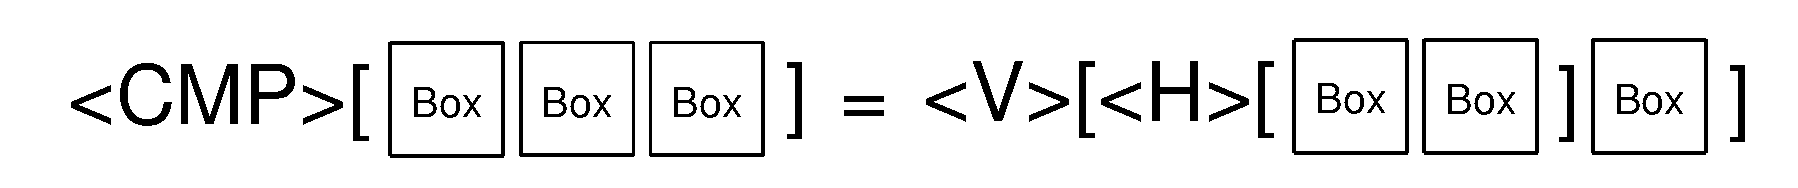
\includegraphics[scale=0.4]{pictures/MacroOperator.eps}
\label{MacroOperator}
\end{figure}
\noindent

\vspace{20mm}


%%% Seznam literatury
%%%
%%% Literatura se řadí abecedně. Úvádí se pouze literatura, na kterou se v textu odkazuje.
%%% Při odkazu na knihu se vždy uvádějí čísla stránek.

\newcommand{\bibitemiso}[3]{\bibitem{#1} #2: \textit{#3}}

\begin{thebibliography}{99}
\addcontentsline{toc}{chapter}{Bibliography}

\bibitemiso{Xtext}{Itemis AG}{Xtext Framework}, [online], 2012 [cit. 2012-07-15]. $<$\url{http://www.eclipse.org/Xtext/}$>$

\bibitemiso{Eclipse}{The Eclipse Foundation}{Eclipse IDE}, [online], 2012 [cit. 2012-07-15]. $<$\url{http://www.eclipse.org/}$>$

\bibitemiso{EPL}{Wikipedia}{Eclipse Public License}, [online], 2012 [cit. 2012-07-15]. $<$\url{http://en.wikipedia.org/wiki/Eclipse_Public_License}$>$

\bibitemiso{EMF}{The Eclipse Foundation}{The Eclipse Modeling Framework Project (EMF)}, [online], 2012 [cit. 2012-07-15]. $<$\url{http://www.eclipse.org/modeling/emf/}$>$

\bibitemiso{POJO}{Wikipedia}{Plain Old Java Object}, [online], 2012 [cit. 2012-07-15]. $<$\url{http://en.wikipedia.org/wiki/Plain_Old_Java_Object}$>$

\bibitemiso{Guice}{Google}{Google Guice}, [online], 2012 [cit. 2012-07-15]. $<$\url{http://code.google.com/p/google-guice/}$>$

\bibitemiso{URI}{Wikipedia}{Uniform Resource Identifier}, [online], 2012 [cit. 2012-07-15]. $<$\url{http://en.wikipedia.org/wiki/Uniform_resource_identifier}$>$

\bibitemiso{AST}{Wikipedia}{Abstract Syntax Tree}, [online], 2012 [cit. 2012-07-15]. $<$\url{http://en.wikipedia.org/wiki/Abstract_syntax_tree}$>$

\bibitemiso{StrategoXT}{Eelco Visser}{Stratego/XT Tutorial Chapter 9.}, [online], 2008 [cit. 2012-09-03]. $<$\url{http://releases.strategoxt.org/strategoxt-manual/unstable/manual/chunk-chapter/generic-pretty-printing.html#pp-table}$>$

\bibitemiso{Metaprogramming}{Wikipedia}{Metaprogramming}, [online], 2012 [cit. 2012-09-03]. $<$\url{http://en.wikipedia.org/wiki/Metaprogramming}$>$

\bibitemiso{PPML}{INRIA Sophia Antipolis}{The CtCoq System}, [online], 2012 [cit. 2012-09-03]. $<$\url{http://www-sop.inria.fr/croap/ctcoq/help/notations.html}$>$

\bibitemiso{Brand-Visser}{Eelco Visser , Mark van den Brand}{Generation of Formatters for Context-free Languages}, [PDF file, online], 1999 [cit. 2012-09-03]. $<$\url{http://citeseerx.ist.psu.edu/viewdoc/summary?doi=10.1.1.47.4257}$>$

\bibitemiso{DeJonge}{Merijn de Jonge}{A PrettyPrinter for Every Occasion}, [PDF file, online], 2000 [cit. 2012-09-03]. $<$\url{http://reference.kfupm.edu.sa/content/p/r/a_pretty_printer_for_every_occasion__188340.pdf}$>$

\bibitemiso{OCaml}{Pierre Weis}{How to Pretty-print (to Use ``format'' ?) ?l}, [online], 1996 [cit. 2012-09-03]. $<$\url{http://caml.inria.fr/pub/old_caml_site/FAQ/format-eng.html}$>$

\bibitemiso{SDF}{J. Heering, P. R. H. Hendriks, P. Klint, J. Rekers}{The Syntax Definition Formalism SDF - Reference Manual}, [PDF file, online], 1989 [cit. 2012-09-03]. $<$\url{http://pdf.aminer.org/001/067/569/the_syntax_definition_formalism_sdf_reference_manual.pdf}$>$

\bibitemiso{Centaur}{P. Borras, D. Clément, Th. Despeyroux, J. Incerpi, G. Kahn, B. Lang, V. Pascual}{CENTAUR: The System}, [PDF file, online], 1988 [cit. 2012-09-03]. $<$\url{http://dl.acm.org/citation.cfm?id=65005}$>$

\bibitemiso{DeJongePhD}{Merijn de Jonge}{To Reuse or To Be Reused}, Amsterdam: University of Amsterdam, Faculty of Science, FNWI: Informatics Institute (II),  Supervisor:~P.~Klint. Co-promotor:~A.~van~Deursen, 2003.  [cit. 2012-09-03], page 51-72

\bibitemiso{DFS}{Wikipedia}{Depth-first Search}, [online], 2012 [cit. 2012-09-03]. $<$\url{http://en.wikipedia.org/wiki/Depth-first_search}$>$

\bibitemiso{Xtend}{Itemis AG}{Xtend 2}, [online], 2012 [cit. 2012-09-03]. $<$\url{http://www.eclipse.org/Xtend/}$>$

\bibitemiso{XPand}{The Eclipse Foundation}{XPand2}, [online], 2012 [cit. 2012-09-03]. $<$\url{http://help.eclipse.org/galileo/index.jsp?topic=/org.eclipse.xpand.doc/help/ch01s06.html}$>$

\bibitemiso{Acceleo}{The Eclipse Foundation}{Acceleo}, [online], 2012 [cit. 2012-09-03]. $<$\url{http://wiki.eclipse.org/Acceleo}$>$

\bibitemiso{Xtend1}{openarchitectureware.org}{Xtend}, [online], 2012 [cit. 2012-09-03]. $<$\url{http://www.openarchitectureware.org/pub/documentation/4.3.1/html/contents/core_reference.html#Xtend_language}$>$

\bibitemiso{XMI}{Object Management Group}{OMG MOF 2 XMI Mapping Specification}, [PDF file, online], August  2011 [cit. 2012-09-03]. $<$\url{http://www.omg.org/spec/XMI/2.4.1/PDF/}$>$

\bibitemiso{XtextCommunity}{Itemis AG}{What Others Have Built with Xtext}, [online], 2012 [cit. 2012-09-03]. $<$\url{http://www.eclipse.org/Xtext/community.html}$>$

\bibitemiso{Protobuf}{Cedric Vidal}{Protobuf4e}, [online], 2012 [cit. 2012-09-03]. $<$\url{http://code.google.com/p/protobuf4e/}$>$

\bibitemiso{Xtexttypesystem}{Markus Voelter}{Xtext-typesystem}, [online], 2012 [cit. 2012-09-03]. $<$\url{http://code.google.com/a/eclipselabs.org/p/xtext-typesystem/}$>$

\bibitemiso{XTypeS}{Lorenzo Bettini}{XTypeS}, [online], 2012 [cit. 2012-09-03]. $<$\url{http://xtypes.sourceforge.net/}$>$

\bibitemiso{Postprocess}{The Eclipse Foundation}{How Can I Control the Xtext Meta-model Inference}, [online], 2012 [cit. 2012-09-03]. $<$\url{http://wiki.eclipse.org/Xtext/FAQ#How_can_I_control_the_Xtext_meta_model_inference.C2.A0.3F}$>$

\bibitemiso{GenerationGap}{Lake Thoreau}{Generation Gap}, [online], 2012 [cit. 2012-09-03]. $<$\url{http://www.eclipsecon.org/2012/category/tags/generation-gap}$>$

\bibitemiso{WorkbenchProjects}{languageworkbenches.net}{LWC2011 Comparison Matrix}, [online], 2012 [cit. 2012-09-03]. $<$\url{http://www.languageworkbenches.net/index.php?title=LWC2011_Comparison_Matrix}$>$

\bibitemiso{GMP}{The Eclipse Foundation}{Graphical Modeling Project (GMP)}, [online], 2012 [cit. 2012-09-03]. $<$\url{http://www.eclipse.org/modeling/gmp/}$>$ 

\bibitemiso{MetaEdit}{MetaCase}{MetaEdit+ Domain-specific Modeling (DSM) environment}, [online], 2012 [cit. 2012-09-03]. $<$\url{http://www.eclipse.org/modeling/gmp/}$>$ 

\bibitemiso{ObeoDesigner}{Obeo}{Obeo Designer}, [online], 2012 [cit. 2012-09-03]. $<$\url{http://www.obeodesigner.com/}$>$ 

\bibitemiso{DslTools}{Microsoft}{DSL Tools Home on Code Gallery}, [online], 2012 [cit. 2012-09-03]. $<$\url{http://archive.msdn.microsoft.com/DslTools}$>$ 

\bibitemiso{EMFText}{DevBoost}{EMFText}, [online], 2012 [cit. 2012-09-03]. $<$\url{http://www.emftext.org/index.php/EMFText}$>$ 

\bibitemiso{MPS}{JetBrains}{Meta Programming System}, [online], 2012 [cit. 2012-09-03]. $<$\url{http://www.jetbrains.com/mps/}$>$ 

\end{thebibliography}

\newpage
\addappheadtotoc
\appendix \chapter{Content of Attached CD-ROM}
This thesis is accomponied by the CD-ROM containing source code of the prototype implementation and another affairs related to this thesis. The structure of CD-ROM's content is organized as follows.: 	

\begin{cdcontentlist}
 	\member{/README.txt}{A brief description of the content of the CD-ROM.}
	\member{/Code/}{The directory contains source codes of prototype's implementation. Further,a workflow for the \textsc{Eclipse} is present  that  allows for browsing following prototype's projects comfortably.}
	\begin{cdcontentlist}
		\member{gpp}{The project contains an implementation of  behavior of operators, fragments dedicated for MWE, the generic code formatter, the generic syntax highlighter and another mentioned functionalites unrelated to the creation of some language.}
		\member{gpp.boxmodel}{The project contains the grammar of the \textsc{ModelLang} language and an implementation of runtime concepts for this language.}
		\member{gpp.boxmodel.ui}{The project realizes IDE concepts for the \textsc{ModelLang} language.}
		\member{gpp.boxmodel.operators}{The project contains the grammar of the \textsc{MetaModLang} language and an implementation of runtime concepts for this language.}
		\member{gpp.boxmodel.operators.ui}{The project realizes IDE concepts for the \textsc{MetaModLang} language.}
		\member{gpp.boxmodel.defaultboxmodel}{The project contains the grammar of the \textsc{HeurLang} language and an implementation of runtime concepts for this language.}
		\member{gpp.boxmodel.defaultboxmodel.ui}{The project realizes IDE concepts for the \textsc{HeurLang} language.}
	\end{cdcontentlist}
	\member{/Evaluation/} {The directory contains projects serving as a subject for testing and evaluating the prototype.}
	\member{/Evaluation/Workflow/} {The directory contains  projects defining languages dedicated for testing and a workflow for the \textsc{Eclipse} that allows for using the prototype and browse following projects comfortably.}
	\begin{cdcontentlist}
		\member{cz.gpp}{The project contains the grammar intorduced in the \textit{Section \ref{grammar}} and an implementation of runtime concepts for the corresponding language.}
		\member{cz.gpp.ui}{The project realizes IDE concepts for the language whose grammar was introduced in the \textit{Section \ref{grammar}}.}
		\member{cz.gpp.zoo}{The project contains the grammar intorduced in the \textit{Figure \ref{ModelAndCode}} and an implementation of runtime concepts for the corresponding language.}
		\member{cz.gpp.zoo.ui}{The project realizes IDE concepts for the language whose grammar was introduced in the \textit{Figure \ref{ModelAndCode}}.}
		\member{gpp.tests.operators}{The project contains the grammar of the \textsc{MetaModLang} language and an implementation of runtime concepts for this language.}
		\member{gpp.tests.operators.ui}{The project realizes IDE concepts for the \textsc{MetaModLang} language.}
		\member{biz.vidal.protobuf4e.dsl}{The project contains the grammar from the \textsc{Protobuf4e} project \cite{Protobuf} and an implementation of runtime concepts for the corresponding language.}
		\member{biz.vidal.protobuf4e.dsl.ui}{The project realizes IDE concepts for a language containted in the \textsc{Protobuf4e} project \cite{Protobuf}.}
		\member{expr}{The project contains the grammar from the \textsc{Xtext-typesystem} project \cite{Xtexttypesystem} and an implementation of runtime concepts for the corresponding language.}
		\member{expr.ui}{The project realizes IDE concepts for a language containted in the \textsc{Xtext-typesystem} project \cite{Xtexttypesystem}.}
		\member{it.xtypes}{The project contains the grammar from the \textsc{XTypeS} project \cite{XTypeS} and an implementation of runtime concepts for the corresponding language.}
		\member{it.xtypes.ui}{The project realizes IDE concepts for a language containted in the \textsc{XTypeS} project \cite{XTypeS}.}
	\end{cdcontentlist}
	\member{/Evaluation/Testing/} {The directory contains code dedicated to be pretty-printed by the prototype and a workflow for the \textsc{Eclipse} that allows for pretty-printing code by the prototype and browse following projects comfortably.}
	\begin{cdcontentlist}
		\member{cz.gpp.tests}{The project contains code that is dedicated to be pretty-printed by the protope and matches the grammar intorduced in the \textit{Section~\ref{grammar}}.}
		\member{cz.gpp.zoo.tests}{The project contains code that is dedicated to be pretty-printed by the protope and matches the grammar intorduced in the \textit{Figure~\ref{ModelAndCode}}.}
		\member{gpp.tests.operators.tests}{The project contains code that is dedicated to be pretty-printed by the protope and matches the grammar of the \textsc{MetaModLang} language.}
		\member{biz.vidal.protobuf4e.dsl.tests}{The project contains code that is dedicated to be pretty-printed by the protope and matches the grammar contained in the \textsc{Protobuf4e} project \cite{Protobuf}.}
		\member{expr.xample}{The project contains code that is dedicated to be pretty-printed by the protope and matches the grammar contained in the \textsc{Xtext-typesystem} project \cite{Xtexttypesystem}.}
		\member{it.xtypes.examples}{The project contains code that is dedicated to be pretty-printed by the protope and matches the grammar contained in the \textsc{XTypeS} project \cite{XTypeS}.}
	\end{cdcontentlist}
	\member{/Document/}{The directory contains an electronic version of this thesis.}
	\member{/Prerequisities/}{The directory contains a description of software items for the \textsc{Eclipse Indigo} that are neccessary for running the prototype suchas the \textsc{Eclipse Modeling Tools}, the \textsc{Xpand SDK}, the \textsc{Xtext SDK}. This description can be imported into the \textsc{Eclipse}, which will run the installation of the software items.}
 \end{cdcontentlist}


\end{document}

